\input{preamble.tex}

\title{Circuitos digitais}

\institute{Universidade Estadual Paulista Júlio de Mesquita Filho}

\author{André Furlan - andre.furlan@unesp.br}

\logo{\includegraphics[height=1cm]{unesp.png}}
\date{\the\year}

\begin{document}
	
	\frame{\titlepage}
	
	\section{Sistema binário, álgebra de Boole e lógica}
		\begin{frame}
	\frametitle{Números binários}
	\begin{columns}
		\column{0.6\textwidth}
			\par Vantagens
			\begin{itemize}
				\item Dois estados (mais difícil deteriorar)
				\item Discretos
				\item Manipulação algébrica (álgebra de Boole)
			\end{itemize}
		\column{0.4\textwidth}
			\par Desantagens
			\begin{itemize}
				\item Dois estados em oposição a infinitos estados
				\item Discretos em oposição a contínuo
			\end{itemize}
	\end{columns}
	\par Mundo ideal: Junção do analógico com o digital
\end{frame}


\begin{frame}
	\frametitle{Sistema numérico posicional}
	
	\begin{columns}
		\column{0.5\textwidth}
			\par Dada a base com uma certa quantidade de elementos $B$ e símbolos $d \in D = \{d_0, \dots, d_n \}$, então um valor numérico decimal $V$ \textbf{posicional} pode ser representado por 
			\begin{equation}
				V(B) = \sum_{i=0}^{n} d_i . B^{n - i}
			\end{equation}
			\par Sendo $||$ o operador de cardinalidade então $n=|D| - 1$ \newline
		\column{0.5\textwidth}
			\only<1>{
				\par Por exemplo, para o número \textbf{decimal} 249:
				\par $B=10$ 
				\par $D = \{2,4,9\} \implies |D| = 3 \implies n = 2$
				\begin{equation}
					\begin{aligned}
						&V(10) = \sum_{i=0}^{2} d_i . 10^{2-i} = \\
						&d_0 . 10^{2-0} + d_1 . 10^{2-1} + d_2 . 10^{2-2} = \\
						&2 . 10^2 + 4 . 10^1 + 9 . 10^0 = \\
						&\boxed{2.100 + 4.10 + 9.1 = 249}
					\end{aligned}
				\end{equation}
			}
			\only<2>{
				\par Por exemplo, para o número \textbf{binário} 11:
				\par $B=2$ 
				\par $D = \{1,1\} \implies |D| = 2 \implies n = 1$
				\begin{equation}
					\begin{aligned}
						&V(2) = \sum_{i=0}^{1} d_i . 2^{1-i} = \\
						&d_0.2^{1-0} + d_1.2^{1-1} = \\
						&1.2^1 + 1.2^0 = \\
						&\boxed{2+1 = 3}
					\end{aligned}
				\end{equation}
			}
	\end{columns}
\end{frame}

\begin{frame}
	\frametitle{Circuitos lógicos e algébra Booleana}
	\par Antes de avançarmos no estudo e na representação de circuitos lógicos, vamos entender como os estados de "ligado" e "desligado" dos componentes podem ser utilizados para gerar resultados úteis. Portanto, antes de abordarmos esses tópicos, faremos uma imersão na álgebra booleana, explorando tabelas verdade e formas de composição.
\end{frame}

\begin{frame}
	\frametitle{Álgebra de Boole: Operadores \textbf{AND}, \textbf{OR} e \textbf{NOT}}
	\par Sendo o sistema binário posicional aplica-se a ele muitas das regras as quais podemos aplicar aos números decimais o que nos leva a Álgebra de Boole e seus operadores:\newline
	
	\only<1>{
		\begin{columns}
			\column{0.6\textwidth}
				\par \textbf{AND} denotado como \textbf{.} ou $\land$\newline
				\par O operador \textbf{AND} é uma função de 2 variáveis definida como:
				\begin{equation}
					\begin{aligned}
						&AND(a,b) = a.b \\
						&AND(a,b) = 1, \forall a=b=1 \\
						&AND(a,b) = 0, \forall a \neq b \\
					\end{aligned}
				\end{equation}
			\column{0.4\textwidth}
				\begin{table}[h!]
					\centering
					\begin{tabular}{|c|c|c|c|}
						\hline
						a & b & a . b \\ \hline
						0 & 0 & 0     \\ \hline
						0 & 1 & 0     \\ \hline
						1 & 0 & 0     \\ \hline
						1 & 1 & 1     \\ \hline
					\end{tabular}
				    \caption{Tabela verdade para \textbf{AND}.}
					\label{tab:tabelaVerdadeAND}
				\end{table}
		\end{columns}
	}
	\only<2>{
		\begin{columns}
			\column{0.6\textwidth}
				\par \textbf{OR} denotado com \textbf{+} ou $\lor$\newline
				\par O operador \textbf{OR} é uma função de 2 variáveis definida como:
				\begin{equation}
					\begin{aligned}
						&OR(a,b) = a + b \\
						&OR(a,b) = 0, \forall a=b=0 \\
						&OR(a,b) = 1, \forall a \neq b, a=b=1 \\
					\end{aligned}
				\end{equation}
			\column{0.4\textwidth}
			\begin{table}[h!]
				\centering
				\begin{tabular}{|c|c|c|c|}
					\hline
					a & b & a + b \\ \hline
					0 & 0 & 0     \\ \hline
					0 & 1 & 1     \\ \hline
					1 & 0 & 1     \\ \hline
					1 & 1 & 1     \\ \hline
				\end{tabular}
    			\caption{Tabela verdade para \textbf{OR}.}
				\label{tab:tabelaVerdadeOR}
			\end{table}
		\end{columns}
	}
	
	\only<3>{
		\begin{columns}
			\column{0.6\textwidth}
			\par \textbf{NOT} denotado com $\overline{a}$ ou $\neg a$\newline
			\par O operador \textbf{NOT} é uma função de 1 variável definida como:
			\begin{equation}
				\begin{aligned}
					&NOT(a) = \overline{a} \\
					&NOT(a) = 0, \forall a=1 \\
					&NOT(a) = 1, \forall a=0 \\
				\end{aligned}
			\end{equation}
			\column{0.4\textwidth}
			\begin{table}[h!]
				\centering
				\begin{tabular}{|c|c|}
					\hline
					a & $\overline{a}$ \\ \hline
					0 & 1  \\ \hline
					1 & 0 \\ \hline
				\end{tabular}
				\caption{Tabela verdade para \textbf{NOT}.}
				\label{tab:tabelaVerdadeNOT}
			\end{table}
		\end{columns}
	}
\end{frame}

\begin{frame}
	\frametitle{Álgebra de Boole: Composição de de operadores}
	\par É importante destacar que assim com na álgebra tradicional os operadores tem prioridade no momento de sua aplicação na seguinte ordem: \textbf{NOT}, \textbf{AND} e por fim \textbf{OR}. Se usarmos os sinais as regras ficam bem parecidas com a álgebra tradicional: $\overline{a}$, $.$ e $+$.\newline
	
	\begin{columns}
		\column{0.4\textwidth}
			\par A partir dos operadores apresentados vamos brincar um pouquinho com eles:
			\begin{equation}
				(a + b) . c
			\end{equation}
		\column{0.6\textwidth}
			\begin{table}[h!]
				\centering
				\begin{tabular}{|c|c|c|c|c|}
					\hline
					a & b & c & a+b & \(a + b\) . c\\ \hline
					0 & 0 & 0 & 0 & 0 \\ \hline
					0 & 0 & 1 & 0 & 0 \\ \hline
					0 & 1 & 0 & 1 & 0 \\ \hline
					0 & 1 & 1 & 1 & 1 \\ \hline
					1 & 0 & 0 & 1 & 0 \\ \hline
					1 & 0 & 1 & 1 & 1 \\ \hline
					1 & 1 & 0 & 1 & 0 \\ \hline
					1 & 1 & 1 & 1 & 1 \\ \hline
				\end{tabular}
				\caption{Tabela verdade para \textbf{(a + b) . c}.}
				\label{tab:tabelaVerdadeComposta01}
			\end{table}
	\end{columns}
\end{frame}

\begin{frame}
	\frametitle{Álgebra de Boole: Composição de operadores NAND e NOR}
	\begin{center}
		Alguns operadores comuns são compostos: 
	\end{center}
	\begin{columns}
		\column{0.5\textwidth}
		
			\par O operador \textbf{NAND} (NOT AND) é definido segundo a seguinte tabela verdade:
		
			\begin{table}[h!]
				\centering
				\begin{tabular}{|c|c|c|c|c|}
					\hline
					a & b & a . b & $\overline{a . b}$ \\ \hline
					0 & 0 & 0     & 1  \\ \hline
					0 & 1 & 0     & 1  \\ \hline
					1 & 0 & 0     & 1  \\ \hline
					1 & 1 & 1     & 0  \\ \hline
				\end{tabular}
				\caption{Tabela verdade para \textbf{NAND}.}
				\label{tab:tabelaVerdadeNAND}
			\end{table}
		
		\column{0.5\textwidth}
			\par O operador \textbf{NOR} (NOT OR) é definido segundo a seguinte tabela verdade:
			\begin{table}[h!]
				\centering
				\begin{tabular}{|c|c|c|c|c|}
					\hline
					a & b & a + b & $\overline{a + b}$ \\ \hline
					0 & 0 & 0     & 1  \\ \hline
					0 & 1 & 1     & 0  \\ \hline
					1 & 0 & 1     & 0  \\ \hline
					1 & 1 & 1     & 0  \\ \hline
				\end{tabular}
				\caption{Tabela verdade para \textbf{NOR}.}
				\label{tab:tabelaVerdadeNOR}
			\end{table}
	\end{columns}
\end{frame}

\begin{frame}
	\frametitle{Álgebra de Boole: Expressão booleanas equivalentes}
	\par Uma expressão boleana equivalente é aquela que, dada uma mesma entrada, retorna exatamente o mesmo resultado. Expressões boleanas equivalentes podem ser ou não a versão otimizada uma da outra.\newline
	
	\par O que foi dito acima só é possível se alguns \textbf{axiomas}\footnote[frame]{hipóteses básicas ou pré-supostos baseados na experiência empírica ou filosófica} forem definidos. 
	\par A partir desses axiomas podemos definir \textbf{teoremas}\footnote[frame]{Teoremas são proposições demonstráveis a partir dos axiomas}.\newline
	\par Veremos ambos no próximo slide.
\end{frame}

\begin{frame}
	\label{frm:axiomasETeoremas}
	\frametitle{Álgebra de Boole: Expressão booleanas equivalentes}
	\framesubtitle{Axiomas e teoremas}
	\begin{columns}
		\column{0.5\textwidth}
			\par Axiomas:
			\begin{enumerate}
				\item $0.0=0$
				\item $1.1=1$
				\item $0.1=1.0=0$
				\item $1+1=1$
				\item $0+0=0$
				\item $1+0=0+1=1$
				\item $x=0 \implies \overline{x}=1$
				\item $x=1 \implies \overline{x}=0$
		\end{enumerate}
		\column{0.5\textwidth}
			\par Teoremas para AND
			\begin{enumerate}
				\item $x.0=0$
				\item $x.1=x$
				\item $x.x=x$
				\item $x.\overline{x}=0$
			\end{enumerate}
			
			\par Teoremas para OR
			\begin{enumerate}
				\item $x+1=1$
				\item $x+0=x$
				\item $x+x=x$
				\item $x+\overline{x}=1$
			\end{enumerate}
			
			\par Teorema para NOT
			\begin{enumerate}
				\item $\overline{(\overline{x})}=x$
			\end{enumerate}
	\end{columns}
\end{frame}


\begin{frame}
	\frametitle{Álgebra de Boole: Expressão booleanas equivalentes}
	\framesubtitle{Princípio da dualidade}
	\par Dada uma expressão lógica que expressa uma igualdade então é possível criar uma \textbf{expressão dual} na qual a igualdade continua verdadeira.\newline
	
	\par Uma expressão dual é obtida quando se troca os valores de 0 para 1, de 1 para 0 e os operadores de and para or e de or para and. Perceba que \textbf{o resultado da expressão pode mudar} porém a \textbf{igualdade é preservada}.\newline
	
	\par Voltando ao slide \ref{frm:axiomasETeoremas} você perceberá que os teoremas para \textit{OR} são \textbf{dualidades de uma variável} dos teoremas de \textit{AND} e vice-versa.
		
\end{frame}

\begin{frame}
	\frametitle{Álgebra de Boole: Expressão booleanas equivalentes}
	\framesubtitle{Dualidade de duas variáveis}
	\begin{equation}
		\begin{aligned}
			x.y=y.x &\Leftrightarrow x+y=y+x \text{ comutacao}\\
			x+(x.y)=x &\Leftrightarrow x.(x+y) = x \text{ absorcao}\\
			(x.y)+(x.\overline{y})=x &\Leftrightarrow (x+y).(x+\overline{y})=x \text{ combinacao}\\
			\boxed{\text{Teorema de De Morgan: } \overline{(x.y)}=\overline{x}+\overline{y}} &\Leftrightarrow \overline{(x+y)}=\overline{x}.\overline{y}\\
			x+(\overline{x}.y)=x+y &\Leftrightarrow x.(\overline{x}+y)=x.y
		\end{aligned}
	\end{equation}
\end{frame}

\begin{frame}
	\frametitle{Álgebra de Boole: Expressão booleanas equivalentes}
	\framesubtitle{Dualidade de três variáveis}
	\begin{equation}
		\begin{aligned}
			x.(y.z)=(x.y).z &\Leftrightarrow x+(y+z)=(x+y)+z \text{ associação} \\
			x.(y+z)=(x.y)+(x.z) &\Leftrightarrow x+(y.z)=(x+y).(x+z) \text{ distribuição}\\
			(x.y)+(y.z)+(\overline{x}.z)=(x.y)+(\overline{x}.z) &\Leftrightarrow (x+y).(y+z).(\overline{x}+z) = (x+y).(\overline{x}+z) \\ \text{ consenso (sumiço :D)}
		\end{aligned}
	\end{equation}
	\par Em tempo: Eu sei que em alguns lugares tem parenteses sobrando, isso foi intencional pra facilitar a visualização das relações.
\end{frame}

\begin{frame}
	\frametitle{Teorema de D.Morgan}
	
	\definecolor{destaque1}{rgb}{0, 1, 0}
	\definecolor{destaque2}{rgb}{0, 1, 1}
	
	\begin{table}[h]
		\centering
		\caption{Prova exaustiva do teorema de De Morgan: $\overline{(x . y)} = \overline{x} + \overline{y}$}
		\begin{tabular}{|c|c|c|>{\columncolor{destaque1}}c|c|c|>{\columncolor{destaque1}}c|}
			\hline
			$x$ & $y$ & $x . y$ & $\overline{x . y}$ & $\overline{x}$ & $\overline{y}$ & $\overline{x} + \overline{y}$ \\ \hline 
			0 & 0 & 0   & 1 & 1  & 1  & 1 \\ \hline
			0 & 1 & 0   & 1 & 1  & 0  & 1 \\ \hline
			1 & 0 & 0   & 1 & 0  & 1  & 1 \\ \hline
			1 & 1 & 1   & 0 & 0  & 0  & 0 \\ \hline
		\end{tabular}
	\end{table}
	
	\begin{table}[h]
		\centering
		\caption{Prova exaustiva para o dual do teorema de De Morgan: $\overline{(x + y)} = \overline{x} . \overline{y}$}
		\begin{tabular}{|c|c|c|>{\columncolor{destaque2}}c|c|c|>{\columncolor{destaque2}}c|}
			\hline
			$x$ & $y$ & $x + y$ & $\overline{x + y}$ & $\overline{x}$ & $\overline{y}$ & $\overline{x} . \overline{y}$ \\ \hline 
			0 & 0 & 0  & 1   & 1  & 1  & 1 \\ \hline
			0 & 1 & 1  & 0   & 1  & 0  & 0 \\ \hline
			1 & 0 & 1  & 0   & 0  & 1  & 0 \\ \hline
			1 & 1 & 1  & 0   & 0  & 0  & 0 \\ \hline
		\end{tabular}
	\end{table}	
\end{frame}

\begin{frame}
	\frametitle{Provas de expressões na álgebra de Boole }
	
	\begin{itemize}
		\item indução perfeita: Devido a pequena quantidade de valores possíveis (0 ou 1) geralmente é viável provar as igualdades dessa forma. A indução perfeita (prova exaustiva) se dá ao fazer a tabela verdade da igualdade, verificando se os valores literais realmente coincidem. Quando a expressão começa a ter muitas variáveis e/ou se tornar muito grande, esse método pode se tornar inviável devido a grande quantidade de estados possíveis que o sistema pode ter.
		\item manipulação algébrica: Levando em consideração os axiomas e teoremas é possível manipular as igualdades de forma que a igualdade seja provada.
		\item diagrama de Ven: \textit{Nos próximos capítulos}.
	\end{itemize}
\end{frame}

\begin{frame}
	\frametitle{Provas de expressões na álgebra de Boole com diagrama de Venn }
	\par Se interpretarmos \textbf{AND} ou \textbf{.} como $\cap$ e \textbf{OR} ou \textbf{+} como $\cup$ é possível fazer a prova de uma igualdade usando o diagrama de Venn.
	
	\begin{columns}
		\column{.5\linewidth}
		\par Para começar, uma dica interessante é representar as relações do espaço para identificar cada uma das regiões de acordo com a expressão avaliada.
		\begin{figure}
			\centering
			\includegraphics[width=.7\linewidth]{images/relacoesGerais}
			\caption{Relações de um espaço com duas variáveis}
			\label{fig:relacoesgerais}
		\end{figure}
		\column{.5\linewidth}
		\par A partir disso é possível escrever outras relações:
		\begin{equation}
			\begin{aligned}
				(x.\overline{y})+(x.y)&=x \\
				(\overline{x}.y)+(x.y)&=y \\
				(x.\overline{y})+(x.y)+(\overline{x}.y)&=x+y
			\end{aligned}
		\end{equation}
		
	\end{columns}
	
\end{frame}

\begin{frame}
	\frametitle{Provas de expressões na álgebra de Boole com diagrama de Venn }
	\par Como exemplo provaremos o do teorema de DeMorgan: $\overline{(x . y)} = \overline{x}+\overline{y}$
	\begin{columns}
		\column{.5\linewidth}
		\par Lado esquerdo da igualdade.	
		\begin{figure}
			\centering
			\includegraphics[width=0.4\linewidth]{images/x.y}
			\caption{$(x . y)$}
			\label{fig:x}
		\end{figure}
		\begin{figure}
			\centering
			\includegraphics[width=0.4\linewidth]{images/notX.Y}
			\caption{$\overline{(x . y)}$}
			\label{fig:notx}
		\end{figure}
		\column{.5\linewidth}
		\par Lado direito da igualdade.
		\begin{figure}
			\centering
			\includegraphics[width=.9\linewidth]{images/notXNotY}
			\caption{$\overline{x}$ e $\overline{y}$}
			\label{fig:notxnoty}
		\end{figure}
		\begin{figure}
			\centering
			\includegraphics[width=0.4\linewidth]{images/notX+notY-4}
			\caption{$\overline{x}+\overline{y}$}
			\label{fig:notxnoty-4}
		\end{figure}
	\end{columns}
\end{frame}

\begin{frame}
	\frametitle{Provas de expressões na álgebra de Boole com diagrama de Venn }
	\par Como exemplo provaremos $(x.y)+(y.z)+(\overline{x}.z)=(x.y)+(\overline{x}.z) &\Leftrightarrow (x+y).(y+z).(\overline{x}+z) = (x+y).(\overline{x}+z) \text{ consenso (sumiço :D)}$
	\begin{columns}
		\column{.5\linewidth}
		\par Lado esquerdo da igualdade.
		\begin{figure}
			\centering
			\includegraphics[width=0.35\linewidth]{images/x.y+y.z}
			\caption{$(x.y)+(y.z)$}
			\label{fig:xy+yz}
		\end{figure}
		
		\vspace{-2.3em} % Ajusta o espaçamento aqui
		
		\begin{figure}
			\centering
			\includegraphics[width=0.35\linewidth]{images/x.y+y.z+notx.z}
			\caption{$(x.y)+(y.z)+(\overline{x}.z)$}
			\label{fig:x.y+y.z+notx.z}
		\end{figure}
		\column{.5\linewidth}
		\par Lado direito da igualdade.
		\begin{figure}
			\centering
			\includegraphics[width=0.5\linewidth]{images/x.y+notx.z}
			\caption{$(x.y)+(\overline{x}.z)$}
			\label{fig:x.y+notx.z}
		\end{figure}
		
	\end{columns}
\end{frame}

\begin{frame}
	\frametitle{Short test}
	\par A partir dos teoremas e propriedades apresentados mostre que $(x+y).(x+z)=x+y.z$. Indique quais os teoremas e/ou propriedades usados na solução.\newline
	\par Crie dualidades para
	\begin{itemize}
		\item $0.0$
		\item $1.1$
		\item $x=0 \implies \overline{x}=0$
	\end{itemize}
	
%	\begin{figure}
%		\centering
%		\includegraphics[width=0.4\linewidth]{images/shortTest01}
%		\caption{}
%		\label{fig:shorttest01}
%	\end{figure}
	
\end{frame}


\begin{frame}
	\frametitle{Exercícios}
	\only<1>{		
		\par Crie a tabela verdade para a porta lógica AND.
		\par Crie a tabela verdade para a porta lógica OR.
		\par Crie a tabela verdade para a porta lógica NOT.
	}
	\only<2>{
		\par Dada a tabela verdade a seguir, construa a expressão lógica correspondente:
		\begin{center}
			\begin{tabular}{|c|c|c|}
				\hline
				A & B & F \\
				\hline
				0 & 0 & 0 \\
				0 & 1 & 1 \\
				1 & 0 & 1 \\
				1 & 1 & 0 \\
				\hline
			\end{tabular}
		\end{center}
	}
	\only<3>{
		\par Dada a expressão lógica \( F = A \cdot \overline{B} \), desenhe o circuito combinacional correspondente.
	}
	\only<4>{
		\par Dada a expressão lógica \( F = A \cdot B + \overline{A} \cdot \overline{B} \), construa a tabela verdade correspondente.
	}
\end{frame}

\begin{frame}
	\frametitle{Circuitos}
	\par Até agora, revisamos a lógica, as tabelas-verdade e a álgebra booleana. No entanto, ainda não abordamos os circuitos digitais propriamente ditos. A partir de agora, exploraremos a correlação entre as expressões lógicas da álgebra booleana e o projeto de circuitos elétricos.
\end{frame}

\begin{frame}
	\frametitle{Circuitos combinacionais}
	\begin{columns}
		\column{0.6\textwidth}
		\par A chave binária é um componente que permite ou impede a passagem da corrente elétrica dado seus estado. A partir dela criaremos circuitos mais complexos.
		\begin{figure}
			\centering
			\includegraphics[width=0.2\linewidth]{images/chaveBinaria}
			\caption{Chave binária}
			\label{fig:chavebinaria}
		\end{figure}
		\column{0.4\textwidth}
		\par A chave binária pode ser representada de outra forma:
		\begin{figure}
			\centering
			\includegraphics[width=0.7\linewidth]{images/chaveBinariaAbstrata}
			\caption{Chave binária}
			\label{fig:chavebinariaabstrata}
		\end{figure}
	\end{columns}
\end{frame}

\begin{frame}
	\frametitle{Circuitos combinacionais}
	\begin{columns}
		\column{0.6\textwidth}
		\par Agora considere uma função que depende um argumento $x$ para definir seu estado. Tal função pode ser representada no circuito abaixo:
		
		\begin{figure}
			\centering
			\includegraphics[width=0.7\linewidth]{images/funcaoLogica1var}
			\caption{Função lógica de uma variável. No circuito $F$ pode ser ligada a qualquer elemento de saída com um led ou outro circuito.}
			\label{fig:funcaologica1var}
		\end{figure}
		
		\column{0.4\textwidth}
		\par $F = 1 \forall x=1$
		\par $F = 0 \forall x=0$
		\par Portanto $F$ é uma função lógica de \textbf{uma} variável tal que $F(x)=x$
		
	\end{columns}
\end{frame}

\begin{frame}
	\frametitle{Circuitos combinacionais}
	\par A partir de agora é possível construir circuitos mais complexos como \textbf{OR} e \textbf{AND}.
	\begin{columns}
		\column{0.5\textwidth}
		\begin{figure}
			\centering
			\includegraphics[width=0.7\linewidth]{images/portaE}
			\caption{Circuito \textbf{AND}: $a$ e $b$ são suas entradas. Aqui se pode constatar que este circuito pode receber de $2$ a $n$ entradas.}
			\label{fig:portae}
		\end{figure}
		\column{0.5\textwidth}
		\begin{figure}
			\centering
			\includegraphics[width=0.7\linewidth]{images/portaOU}
			\caption{Circuito \textbf{OR}: $a$ e $b$ são suas entradas. Aqui se pode constatar que este circuito pode receber de $2$ a $n$ entradas.}
			\label{fig:portaou}
		\end{figure}
	\end{columns}
\end{frame}

\begin{frame}
	\frametitle{Circuitos combinacionais}
	\par Circuito \textbf{NOT}
	\begin{columns}
		\column{0.5\textwidth}
		\begin{figure}
			\centering
			\includegraphics[width=0.7\linewidth]{images/circuitoNot}
			\caption{Circuito \textbf{NOT}: Inverte a entrada $a$.}
			\label{fig:portanao}
		\end{figure}
		
		\column{0.5\textwidth}
		\par Nada aqui por questões estéticas...
	\end{columns}
\end{frame}

\begin{frame}
	\frametitle{Circuitos combinacionais}
	\par E assim como vimos na álgebra de Boole \textbf{OR} e \textbf{AND} podem ser combinados.
	\begin{figure}
		\centering
		\includegraphics[width=0.7\linewidth]{images/aMaisBVezesC}
		\caption{O \textbf{OR} recebe as entradas $a$ e $b$, o circuito \textbf{AND} recebe $c$ e a saída de \textbf{OR}}
		\label{fig:amaisbvezesc}
	\end{figure}
\end{frame}

\begin{frame}
	\frametitle{Circuitos combinacionais}
	\par Para representar circuitos simples os símbolos já vistos são suficientes, porém, quando a complexidade aumenta pode ficar beeeeeemmmm complicado entender o que se passa. Então precisamos aumentar o nível de abstração encapsulando esse componentes.
\end{frame}

\begin{frame}
	\frametitle{Circuitos combinacionais}
	\begin{figure}
		\centering
		\includegraphics[width=0.7\linewidth]{images/portaEAbstrata}
		\caption{Abstração de circuito \textbf{AND} para a porta \textbf{AND}}
		\label{fig:portaeabstrata}
	\end{figure}
\end{frame}

\begin{frame}
	\frametitle{Circuitos combinacionais}
	\begin{figure}
		\centering
		\includegraphics[width=0.7\linewidth]{images/portaOUAbstrata}
		\caption{Abstração de circuito \textbf{OR} para a porta \textbf{OR}}
		\label{fig:portaouabstrata}
	\end{figure}
\end{frame}

\begin{frame}
	\frametitle{Circuitos combinacionais}
	\begin{figure}
		\centering
		\includegraphics[width=0.7\linewidth]{images/portaNOTAbstrata}
		\caption{Abstração de circuito \textbf{NOT} para a porta \textbf{NOT}}
		\label{fig:portanotabstrata}
	\end{figure}
\end{frame}

\begin{frame}
	\frametitle{Circuitos combinacionais}
	\par Veja como fica o circuito $(a+b).c$ com as novas abstrações.
	\begin{figure}
		\centering
		% Define cores personalizadas
\definecolor{vermelho}{HTML}{FF0000}
\definecolor{verde}{HTML}{00FF00}


\begin{tikzpicture}[circuit logic US, scale=1]
	% Define nós de entrada
	\node (a) at (0,0) {$a$};
	\node (b) [below=0.5cm of a] {$b$};
	\node (c) [below=0.5cm of b] {$c$};
	
	% Define portas lógicas usando coordenadas relativas
	\node (or) [or gate, right=1cm of a.east, yshift=-0.5cm, draw=vermelho, fill=vermelho!20] {};
	\node (and) [and gate, right=1cm of or.output, yshift=-.5cm, draw=verde, fill=verde!20] {};
	
	% Desenhar as conexões
	\draw [draw=black, line width=.3mm] (a.east) -- ++(0.5,0) |- (or.input 1);
	\draw [draw=black, line width=.3mm] (b.east) -- ++(0.5,0) |- (or.input 2);
	
	\draw [draw=black, line width=.3mm] (or.output) -- ++(0.5,0) |- (and.input 1);
	\draw [draw=black, line width=.3mm] (c.east) -- ++(0.5,0) |- (and.input 2);
	\draw [draw=black, line width=.3mm] (and.output) -- ++(0.5,0) node[right] {$\text{saída}$};
\end{tikzpicture}
		\caption{Circuito correspondente a expressão lógica (a+b).c}
		\label{fig:circuitoAndOr}
	\end{figure}
\end{frame}

\begin{frame}
	\frametitle{Exercícios}
	\only<1>{
		\par Dada a expressão lógica \( F = A \cdot \overline{B} \), desenhe o circuito combinacional correspondente.
	}
	\only<2>{
		\par Dada a expressão lógica \( F = A \cdot B + \overline{A} \cdot \overline{B} \), construa a tabela verdade correspondente.
	}
	\only<3>{
		\par Dada a expressão lógica \( F = (A \cdot B + \overline{C}) \cdot (A + C) \), desenhe o circuito combinacional correspondente.
	}
	\only<4>{
		\par Construa a expressão lógica a partir do seguinte circuito combinacional:
		\begin{center}
			\begin{tikzpicture}
				\node (A) at (0,2) {A};
				\node (B) at (0,0) {B};
				\node[and gate US, draw, logic gate inputs=nn] at (2,1) (and1) {};
				\node[or gate US, draw, logic gate inputs=nn] at (4,1) (or1) {};
				
				\draw (A) -| (and1.input 1);
				\draw (B) -| (and1.input 2);
				\draw (A) -- ++(0.5,0) |- (or1.input 1);
				\draw (and1.output) -- (or1.input 2);
				\draw (or1.output) -- ++(1,0) node[right] {F};
			\end{tikzpicture}
		\end{center}
	}
	\only<5>{
		\par Dada a expressão lógica \( F = A + B \cdot \overline{C} \), desenhe o circuito combinacional correspondente.
	}
	\only<6>{
		\par Identifique as portas lógicas utilizadas no seguinte circuito combinacional:
		\begin{center}
			\begin{tikzpicture}
				\node (A) at (0,2) {A};
				\node (B) at (0,0) {B};
				\node[or gate US, draw, logic gate inputs=nn] at (2,1) (or1) {};
				\node[not gate US, draw, logic gate inputs=nn] at (4,1) (not1) {};
				
				\draw (A) -| (or1.input 1);
				\draw (B) -| (or1.input 2);
				\draw (or1.output) -- (not1.input);
				\draw (not1.output) -- ++(1,0) node[right] {F};
			\end{tikzpicture}
		\end{center}
	}
	\only<7>{
		\par Dado o circuito combinacional a seguir, construa a tabela verdade correspondente:
		\begin{center}
			\begin{tikzpicture}
				\node (A) at (0,2) {A};
				\node (B) at (0,0) {B};
				\node[and gate US, draw, logic gate inputs=nn] at (2,1) (and1) {};
				\node[not gate US, draw, logic gate inputs=nn] at (4,1) (not1) {};
				
				\draw (A) -| (and1.input 1);
				\draw (B) -| (and1.input 2);
				\draw (and1.output) -- (not1.input);
				\draw (not1.output) -- ++(1,0) node[right] {F};
			\end{tikzpicture}
		\end{center}
	}
	\only<8>{
		\par Dado o circuito combinacional a seguir, construa a expressão lógica e a tabela verdade correspondente:
		\begin{center}
			\begin{tikzpicture}
				\node (A) at (0,4) {A};
				\node (B) at (0,2) {B};
				\node (C) at (0,0) {C};
				\node[or gate US, draw, logic gate inputs=nn] at (2,3) (or1) {};
				\node[and gate US, draw, logic gate inputs=nn] at (4,1) (and1) {};
				\node[and gate US, draw, logic gate inputs=nn] at (6,3) (and2) {};
				\node[or gate US, draw, logic gate inputs=nn] at (8,2) (or2) {};
				
				\draw (A) -- (or1.input 1);
				\draw (B) -| (or1.input 2);
				\draw (or1.output) -| (and1.input 1);
				\draw (C) -- (and1.input 2);
				\draw (A) -| (and2.input 1);
				\draw (and1.output) -- ++(0.5,0) |- (and2.input 2);
				\draw (and2.output) -- (or2.input 1);
				\draw (B) -| (or2.input 2);
				\draw (or2.output) -- ++(1,0) node[right] {F};
			\end{tikzpicture}
		\end{center}
	}
\end{frame}

		\section{Diagrama de Tempo (\textit{Waveform})}

\begin{frame}{Diagrama de Tempo (\textit{Waveform})}
	\par Quando fazemos o diagrama de tempo ou o \textit{waveform} apresentamos ao circuito uma sequência de  sinais de forma que o circuito responde a essa sequência gerando outras sequências. 
	\begin{itemize}
		\item Mostra os estados do circuito ao longo do tempo.
		\item Permite a visualização do comportamento do circuito durante o tempo.
	\end{itemize}
	\begin{figure}
		\centering
		\includegraphics[width=\linewidth]{images/waveform01}
		\caption{Consegue saber qual porta é esta?}
		\label{fig:waveform01}
	\end{figure}
\end{frame}

\begin{frame}{Prática dirigida 01}
	\par Construção de Circuito a partir de Expressão Algébrica
	\begin{itemize}
		\item Dada a expressão algébrica \(f(x, y, z) = \overline{x} \cdot y + x \cdot \overline{y} \cdot z\), construa: %f=(~x*y)+(x*~y*z)
		\begin{enumerate}
			\item O circuito correspondente usando portas lógicas básicas (AND, OR, NOT).
			\item A tabela verdade que representa o comportamento da função.
			\item O diagrama de tempo (waveform) que mostra os estados do circuito para todas as combinações de \(x\), \(y\) e \(z\) ao longo do tempo.
		\end{enumerate}
	\end{itemize}
	\pause
	\begin{columns}
		\column{.8\linewidth}
			\begin{figure}
				\centering
				% Important: If latex complains about unicode characters,
% please use "\usepackage[utf8x]{inputenc}" in your preamble
% You can change the size of the picture by putting it into the construct:
% 1) \resizebox{10cm}{!}{"below picture"} to scale horizontally to 10 cm
% 2) \resizebox{!}{15cm}{"below picture"} to scale vertically to 15 cm
% 3) \resizebox{10cm}{15cm}{"below picture"} a combination of above two
% It is not recomended to use the scale option of the tikzpicture environment.
 \resizebox{7cm}{!}{
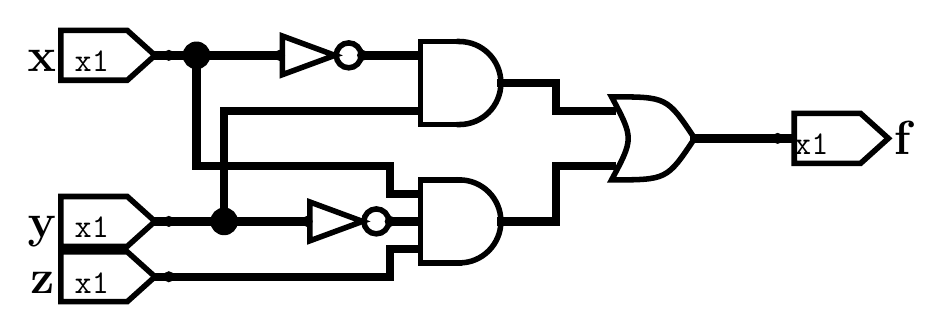
\begin{tikzpicture}[x=1pt,y=-1pt,line cap=rect]
\def\logisimfontA#1{\fontfamily{cmr}{#1}} % Replaced by logisim, original font was "SansSerif"
\def\logisimfontB#1{\fontfamily{cmtt}{#1}} % Replaced by logisim, original font was "Monospaced"
\definecolor{custcol_0_0_0}{RGB}{0, 0, 0}
\definecolor{custcol_ff_ff_ff}{RGB}{255, 255, 255}
\draw [line width=3.0pt, custcol_0_0_0 ]  (246.0,45.0) -- (276.0,45.0) ;
\draw [line width=3.0pt, custcol_0_0_0 ]  (126.0,15.0) -- (146.0,15.0) ;
\draw [line width=3.0pt, custcol_0_0_0 ]  (136.0,75.0) -- (146.0,75.0) ;
\draw [line width=3.0pt, custcol_0_0_0 ]  (96.0,15.0) -- (66.0,15.0) -- (66.0,55.0) -- (136.0,55.0) -- (136.0,65.0) -- (146.0,65.0) ;
\draw [line width=3.0pt, custcol_0_0_0 ]  (106.0,75.0) -- (76.0,75.0) -- (76.0,35.0) -- (146.0,35.0) ;
\fill [line width=3.0pt, custcol_0_0_0]  (76.0,75.0) ellipse (5.0 and 5.0 );
\fill [line width=3.0pt, custcol_0_0_0]  (66.0,15.0) ellipse (5.0 and 5.0 );
\draw [line width=2.0pt, custcol_0_0_0] (161.0,40.0) arc (90.0:-90.0:15.0 and 15.0 );
\draw [line width=2.0pt, custcol_0_0_0 ]  (161.0,10.0) -- (147.0,10.0) -- (147.0,40.0) -- (161.0,40.0) ;
\draw [line width=3.0pt, custcol_0_0_0 ]  (176.0,25.0) -- (196.0,25.0) -- (196.0,35.0) -- (216.0,35.0) -- (216.0,35.0) ;
\draw [line width=3.0pt, custcol_0_0_0 ]  (176.0,75.0) -- (196.0,75.0) -- (196.0,55.0) -- (216.0,55.0) -- (216.0,55.0) ;
\draw [line width=2.0pt, custcol_0_0_0 ]  (246.0,45.0) .. controls  (236.0,30.0)  ..  (216.0,30.0) .. controls  (224.0,45.0)  ..  (216.0,60.0) .. controls  (236.0,60.0)  ..  (246.0,45.0) -- cycle ;
\draw [line width=3.0pt, custcol_0_0_0 ]  (280.0,45.0) -- (277.0,45.0) ;
\draw [line width=2.0pt, custcol_0_0_0 ]  (306.0,36.0) -- (316.0,45.0) -- (306.0,54.0) -- (282.0,54.0) -- (282.0,36.0) -- cycle;
\logisimfontB{\fontsize{12pt}{12pt}\selectfont\node[inner sep=0, outer sep=0, custcol_0_0_0, anchor=base west] at  (282.0,51.0)  {x1};}
\logisimfontA{\fontsize{16pt}{16pt}\fontseries{bx}\selectfont\node[inner sep=0, outer sep=0, custcol_0_0_0, anchor=base west] at  (318.0,51.0)  {f};}
\fill [line width=2.0pt, custcol_0_0_0]  (276.0,45.0) ellipse (2.0 and 2.0 );
\draw [line width=2.0pt, custcol_0_0_0 ]  (116.0,15.0) -- (97.0,8.0) -- (97.0,22.0) -- cycle;
\draw [line width=2.0pt, custcol_0_0_0]  (121.0,15.0) ellipse (4.5 and 4.5 );
\fill [line width=2.0pt, custcol_0_0_0]  (126.0,15.0) ellipse (2.0 and 2.0 );
\fill [line width=2.0pt, custcol_0_0_0]  (96.0,15.0) ellipse (2.0 and 2.0 );
\draw [line width=2.0pt, custcol_0_0_0 ]  (126.0,75.0) -- (107.0,68.0) -- (107.0,82.0) -- cycle;
\draw [line width=2.0pt, custcol_0_0_0]  (131.0,75.0) ellipse (4.5 and 4.5 );
\fill [line width=2.0pt, custcol_0_0_0]  (136.0,75.0) ellipse (2.0 and 2.0 );
\fill [line width=2.0pt, custcol_0_0_0]  (106.0,75.0) ellipse (2.0 and 2.0 );
\draw [line width=2.0pt, custcol_0_0_0] (161.0,90.0) arc (90.0:-90.0:15.0 and 15.0 );
\draw [line width=2.0pt, custcol_0_0_0 ]  (161.0,60.0) -- (147.0,60.0) -- (147.0,90.0) -- (161.0,90.0) ;
\draw [line width=3.0pt, custcol_0_0_0 ]  (51.0,15.0) -- (56.0,15.0) -- (66.0,15.0) ;
\draw [line width=2.0pt, custcol_0_0_0 ]  (41.0,24.0) -- (51.0,15.0) -- (41.0,6.0) -- (17.0,6.0) -- (17.0,24.0) -- cycle;
\logisimfontB{\fontsize{12pt}{12pt}\selectfont\node[inner sep=0, outer sep=0, custcol_0_0_0, anchor=base west] at  (22.0,21.0)  {x1};}
\logisimfontA{\fontsize{16pt}{16pt}\fontseries{bx}\selectfont\node[inner sep=0, outer sep=0, custcol_0_0_0, anchor=base west] at  (5.0,21.0)  {x};}
\fill [line width=2.0pt, custcol_0_0_0]  (56.0,15.0) ellipse (2.0 and 2.0 );
\draw [line width=3.0pt, custcol_0_0_0 ]  (51.0,75.0) -- (56.0,75.0) -- (76.0,75.0) ;
\draw [line width=2.0pt, custcol_0_0_0 ]  (41.0,84.0) -- (51.0,75.0) -- (41.0,66.0) -- (17.0,66.0) -- (17.0,84.0) -- cycle;
\logisimfontB{\fontsize{12pt}{12pt}\selectfont\node[inner sep=0, outer sep=0, custcol_0_0_0, anchor=base west] at  (22.0,81.0)  {x1};}
\logisimfontA{\fontsize{16pt}{16pt}\fontseries{bx}\selectfont\node[inner sep=0, outer sep=0, custcol_0_0_0, anchor=base west] at  (5.0,81.0)  {y};}
\fill [line width=2.0pt, custcol_0_0_0]  (56.0,75.0) ellipse (2.0 and 2.0 );
\draw [line width=3.0pt, custcol_0_0_0 ]  (51.0,95.0) -- (56.0,95.0) -- (136.0,95.0) -- (136.0,85.0) -- (146.0,85.0) ;
\draw [line width=2.0pt, custcol_0_0_0 ]  (41.0,104.0) -- (51.0,95.0) -- (41.0,86.0) -- (17.0,86.0) -- (17.0,104.0) -- cycle;
\logisimfontB{\fontsize{12pt}{12pt}\selectfont\node[inner sep=0, outer sep=0, custcol_0_0_0, anchor=base west] at  (22.0,101.0)  {x1};}
\logisimfontA{\fontsize{16pt}{16pt}\fontseries{bx}\selectfont\node[inner sep=0, outer sep=0, custcol_0_0_0, anchor=base west] at  (6.0,101.0)  {z};}
\fill [line width=2.0pt, custcol_0_0_0]  (56.0,95.0) ellipse (2.0 and 2.0 );
\end{tikzpicture}
}
				\label{fig:exe14}
			\end{figure}
			\begin{figure}
				\centering
				\includegraphics[width=\linewidth]{images/waveform03}
				\label{fig:waveform03}
			\end{figure}
		\column{.2\linewidth}
			\par Tabela verdade:\\
			\begin{tabular}{ccc|c}
				$x$&$y$&$z$&$f$\\
				\hline
				$0$&$0$&$0$&$0$\\
				$0$&$0$&$1$&$0$\\
				$0$&$1$&$0$&$1$\\
				$0$&$1$&$1$&$1$\\
				$1$&$0$&$0$&$0$\\
				$1$&$0$&$1$&$1$\\
				$1$&$1$&$0$&$0$\\
				$1$&$1$&$1$&$0$\\
			\end{tabular}
	\end{columns}
\end{frame}

\begin{frame}{Prática dirigida 02}
	\par Análise de Diagrama de Tempo
	\begin{figure}
		\centering
		\includegraphics[width=0.7\linewidth]{images/waveform02}
		\label{fig:waveform02}
	\end{figure}
	\begin{columns}
		\column{.5\linewidth}
		\begin{itemize}
			\item Considerando o diagrama dado:
			\begin{enumerate}
				\item O circuito que pode gerar o comportamento mostrado no diagrama.
				\item A tabela verdade associada ao circuito.
				\item A expressão algébrica correspondente ao circuito.
			\end{enumerate}
		\end{itemize}
		\pause
		\column{.2\linewidth}
		\par Tabela verdade:
		\begin{center}
			\begin{tabular}{cc|c}
				$x$&$y$&$z$\\
				\hline
				$0$&$0$&$1$\\
				$0$&$1$&$0$\\
				$1$&$0$&$1$\\
				$1$&$1$&$1$\\
			\end{tabular}
		\end{center}		
		\par Expressão:
		$z =  \overline{y} +x$
		\column{.3\linewidth}
		\begin{figure}
			\centering
			% Important: If latex complains about unicode characters,
% please use "\usepackage[utf8x]{inputenc}" in your preamble
% You can change the size of the picture by putting it into the construct:
% 1) \resizebox{10cm}{!}{"below picture"} to scale horizontally to 10 cm
% 2) \resizebox{!}{15cm}{"below picture"} to scale vertically to 15 cm
% 3) \resizebox{10cm}{15cm}{"below picture"} a combination of above two
% It is not recomended to use the scale option of the tikzpicture environment.
\resizebox{4.5cm}{!}{
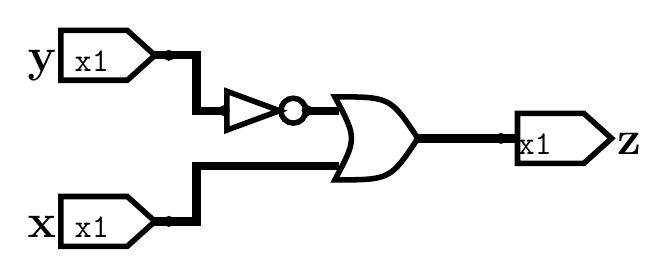
\begin{tikzpicture}[x=1pt,y=-1pt,line cap=rect]
\def\logisimfontA#1{\fontfamily{cmr}{#1}} % Replaced by logisim, original font was "SansSerif"
\def\logisimfontB#1{\fontfamily{cmtt}{#1}} % Replaced by logisim, original font was "Monospaced"
\definecolor{custcol_0_0_0}{RGB}{0, 0, 0}
\definecolor{custcol_ff_ff_ff}{RGB}{255, 255, 255}
\draw [line width=3.0pt, custcol_0_0_0 ]  (146.0,45.0) -- (176.0,45.0) ;
\draw [line width=3.0pt, custcol_0_0_0 ]  (106.0,35.0) -- (116.0,35.0) -- (116.0,35.0) ;
\draw [line width=2.0pt, custcol_0_0_0 ]  (146.0,45.0) .. controls  (136.0,30.0)  ..  (116.0,30.0) .. controls  (124.0,45.0)  ..  (116.0,60.0) .. controls  (136.0,60.0)  ..  (146.0,45.0) -- cycle ;
\draw [line width=2.0pt, custcol_0_0_0 ]  (96.0,35.0) -- (77.0,28.0) -- (77.0,42.0) -- cycle;
\draw [line width=2.0pt, custcol_0_0_0]  (101.0,35.0) ellipse (4.5 and 4.5 );
\fill [line width=2.0pt, custcol_0_0_0]  (106.0,35.0) ellipse (2.0 and 2.0 );
\fill [line width=2.0pt, custcol_0_0_0]  (76.0,35.0) ellipse (2.0 and 2.0 );
\draw [line width=3.0pt, custcol_0_0_0 ]  (180.0,45.0) -- (177.0,45.0) ;
\draw [line width=2.0pt, custcol_0_0_0 ]  (206.0,36.0) -- (216.0,45.0) -- (206.0,54.0) -- (182.0,54.0) -- (182.0,36.0) -- cycle;
\logisimfontB{\fontsize{12pt}{12pt}\selectfont\node[inner sep=0, outer sep=0, custcol_0_0_0, anchor=base west] at  (182.0,51.0)  {x1};}
\logisimfontA{\fontsize{16pt}{16pt}\fontseries{bx}\selectfont\node[inner sep=0, outer sep=0, custcol_0_0_0, anchor=base west] at  (218.0,51.0)  {z};}
\fill [line width=2.0pt, custcol_0_0_0]  (176.0,45.0) ellipse (2.0 and 2.0 );
\draw [line width=3.0pt, custcol_0_0_0 ]  (51.0,75.0) -- (56.0,75.0) -- (66.0,75.0) -- (66.0,55.0) -- (116.0,55.0) -- (116.0,55.0) ;
\draw [line width=2.0pt, custcol_0_0_0 ]  (41.0,84.0) -- (51.0,75.0) -- (41.0,66.0) -- (17.0,66.0) -- (17.0,84.0) -- cycle;
\logisimfontB{\fontsize{12pt}{12pt}\selectfont\node[inner sep=0, outer sep=0, custcol_0_0_0, anchor=base west] at  (22.0,81.0)  {x1};}
\logisimfontA{\fontsize{16pt}{16pt}\fontseries{bx}\selectfont\node[inner sep=0, outer sep=0, custcol_0_0_0, anchor=base west] at  (5.0,81.0)  {x};}
\fill [line width=2.0pt, custcol_0_0_0]  (56.0,75.0) ellipse (2.0 and 2.0 );
\draw [line width=3.0pt, custcol_0_0_0 ]  (51.0,15.0) -- (56.0,15.0) -- (66.0,15.0) -- (66.0,35.0) -- (76.0,35.0) ;
\draw [line width=2.0pt, custcol_0_0_0 ]  (41.0,24.0) -- (51.0,15.0) -- (41.0,6.0) -- (17.0,6.0) -- (17.0,24.0) -- cycle;
\logisimfontB{\fontsize{12pt}{12pt}\selectfont\node[inner sep=0, outer sep=0, custcol_0_0_0, anchor=base west] at  (22.0,21.0)  {x1};}
\logisimfontA{\fontsize{16pt}{16pt}\fontseries{bx}\selectfont\node[inner sep=0, outer sep=0, custcol_0_0_0, anchor=base west] at  (5.0,21.0)  {y};}
\fill [line width=2.0pt, custcol_0_0_0]  (56.0,15.0) ellipse (2.0 and 2.0 );
\end{tikzpicture}
}

			\label{fig:exe09}
		\end{figure}
	\end{columns}
\end{frame}

\section{Mintermos e Maxtermos}

\begin{frame}
	\frametitle{Mintermos e Maxtermos}
	\framesubtitle{Introdução}
	\par Até agora, determinamos as expressões algébricas de forma intuitiva, analisando os circuitos e os resultados das tabelas verdade para, geralmente, identificar a expressão lógica correspondente ao circuito. A partir de agora, utilizaremos ferramentas que oferece um método bem definido para montar a expressão algébrica correspondente ao circuito analisado.
	\par Tais ferramentas se chamam \textit{Mintermos} e \textit{Maxtermos} que, embora não produzam uma expressão otimizada, fornecem uma função inicial que pode ser manipulada e minimizada se assim o desejarmos.
\end{frame}

\begin{frame}
	\frametitle{Mintermos e Maxtermos}
	\framesubtitle{Definição}
	\begin{itemize}
		\item \textbf{Mintermos (Soma de Produtos Canônica (SOP)):} A função é expressa como a soma (OR) das linhas onde a função vale 1.
		\item \textbf{Maxtermos (Produto de Somas Canônica (POS)):} A função é expressa como o produto (AND) das linhas onde a função vale 0.
	\end{itemize}
\end{frame}

\begin{frame}
	\frametitle{Mintermos e Maxtermos}
	\framesubtitle{Definição e propriedades da soma de produtos canônica (SOP)}
	\begin{itemize}
		\item A implementação canônica de uma função booleana que seleciona os produtos das variáveis onde o resultado é 1.
		\item Propriedades:
		\begin{itemize}
			\item Unicidade: Existe uma única SOP canônica para cada função booleana.
			\item Importância: Útil na análise e síntese de circuitos digitais.
			\item Minimização: Pode ser simplificada com Mapas de Karnaugh ou Quine-McCluskey.
		\end{itemize}
	\end{itemize}
\end{frame}

\begin{frame}
	\frametitle{Mintermos e Maxtermos}
	\framesubtitle{Definição e Propriedades do produto de somas canônica (POS)}
	\begin{itemize}
		\item Forma canônica que seleciona as somas das variáveis onde o resultado é 0.
		\item Propriedades:
		\begin{itemize}
			\item Unicidade: Existe uma única POS canônica para cada função booleana.
			\item Importância: Utilizada em design digital para implementar lógica com portas OR e AND.
			\item Minimização: Pode ser simplificada como a SOP canônica.
		\end{itemize}
	\end{itemize}
\end{frame}


\begin{frame}
	\frametitle{Mintermos e Maxtermos}
	\framesubtitle{Exemplo de determinação de função lógica}
	
	\par Vamos determinar a \textbf{função lógica} a partir da tabela verdade abaixo:
	
	\[
	\begin{array}{|c|c|c|c|}
		\hline
		\textbf{a} & \textbf{b} & \textbf{c} & \textbf{f(a, b, c)} \\
		\hline
		0 & 0 & 0 & 0 \\
		0 & 0 & 1 & 1 \\
		0 & 1 & 0 & 0 \\
		0 & 1 & 1 & 1 \\
		1 & 0 & 0 & 1 \\
		1 & 0 & 1 & 1 \\
		1 & 1 & 0 & 0 \\
		1 & 1 & 1 & 0 \\
		\hline
	\end{array}
	\]
\end{frame}

\begin{frame}
	\frametitle{Mintermos e Maxtermos}
	\framesubtitle{Determinação da função lógica usando Mintermos}
	\begin{columns}
		\column{.35\linewidth}
			\par \textcolor{blue}{Mintermos}: Linhas onde $f(a, b, c) = 1$. \\ \textcolor{green}{Maxtermos} Linhas onde $f(a, b, c) = 0$.
			\[
			\begin{array}{|c|c|c|c|}
				\hline
				\textbf{a} & \textbf{b} & \textbf{c} & \textbf{f(a, b, c)} \\
				\hline
				0 & 0 & 0 & \cellcolor{green} 0 \\
				0 & 0 & 1 & \cellcolor{blue} 1 \\
				0 & 1 & 0 & \cellcolor{green} 0 \\
				0 & 1 & 1 & \cellcolor{blue} 1 \\
				1 & 0 & 0 & \cellcolor{blue} 1 \\
				1 & 0 & 1 & \cellcolor{blue} 1 \\
				1 & 1 & 0 & \cellcolor{green} 0 \\
				1 & 1 & 1 & \cellcolor{green} 0 \\
				\hline
			\end{array}
			\]
		\column{.65\linewidth}
			\par \textbf{Passo 1:} Identifique as linhas onde \(f(a, b, c) = 1\).
			\begin{itemize}
				\item 02: \(a = 0\), \(b = 0\), \(c = 1\)  \(\rightarrow\) Mintermo: \(\overline{a}.\overline{b}.c\)
				\item 04: \(a = 0\), \(b = 1\), \(c = 1\)  \(\rightarrow\) Mintermo: \(\overline{a}.bc\)
				\item 05: \(a = 1\), \(b = 0\), \(c = 0\)  \(\rightarrow\) Mintermo: \(a\overline{b}.\overline{c}\)
				\item 06: \(a = 1\), \(b = 0\), \(c = 1\)  \(\rightarrow\) Mintermo: \(a\overline{b}.c\)
			\end{itemize}
			
			\par \textbf{Passo 2:} Escreva a função como a soma (OR) desses mintermos.\newline
			
			\par A função lógica pode ser expressa como a soma dos mintermos correspondentes: \\$\boxed{f(a, b, c) = \overline{a}.\overline{b}.c + \overline{a}bc + a\overline{b}\overline{c} + ab\overline{c}}$
	\end{columns}
	
\end{frame}

\begin{frame}
	\frametitle{Mintermos e Maxtermos}
	\framesubtitle{Determinação da função lógica usando Maxtermos}
	\begin{columns}
		\column{.35\linewidth}
			\par \textcolor{blue}{Mintermos}: Linhas onde $f(a, b, c) = 1$. \\ \textcolor{green}{Maxtermos} Linhas onde $f(a, b, c) = 0$.
			\[
			\begin{array}{|c|c|c|c|}
				\hline
				\textbf{a} & \textbf{b} & \textbf{c} & \textbf{f(a, b, c)} \\
				\hline
				0 & 0 & 0 & \cellcolor{green} 0 \\
				0 & 0 & 1 & \cellcolor{blue} 1 \\
				0 & 1 & 0 & \cellcolor{green} 0 \\
				0 & 1 & 1 & \cellcolor{blue} 1 \\
				1 & 0 & 0 & \cellcolor{blue} 1 \\
				1 & 0 & 1 & \cellcolor{blue} 1 \\
				1 & 1 & 0 & \cellcolor{green} 0 \\
				1 & 1 & 1 & \cellcolor{green} 0 \\
				\hline
			\end{array}
			\]
		\column{.65\linewidth}
			\par \textbf{Passo 1:} Identifique as linhas onde \(f(a, b, c) = 0\).
			\begin{itemize}
				\item 01: \(a = 0\), \(b = 0\), \(c = 0\)  \(\rightarrow\) Maxtermo: \(a + b + c\)
				\item 03: \(a = 0\), \(b = 1\), \(c = 0\)  \(\rightarrow\) Maxtermo: \(a + \overline{b} + c\)
				\item 07: \(a = 1\), \(b = 1\), \(c = 0\)  \(\rightarrow\) Maxtermo: \(\overline{a} + b + c\)
				\item 08: \(a = 1\), \(b = 1\), \(c = 1\)  \(\rightarrow\) Maxtermo: \(\overline{a} + b + \overline{c}\)
			\end{itemize}
			
			\textbf{Passo 2:} Escreva a função como o produto (AND) desses maxtermos.\newline
			
			A função lógica pode ser expressa como o produto dos maxtermos correspondentes:$f(a, b, c) =$ \\ $\boxed{(a + b + c) \cdot (a + \overline{b} + c) \cdot (\overline{a} + b + c) \cdot (\overline{a} + b + \overline{c})}$
		\end{columns}
\end{frame}


\begin{frame}{SOP - Prática guiada 01}
	\begin{itemize}
		\item Considere a função f(a, b, c) definida pela tabela verdade:
		\item \textbf{tabela verdade:}
		\begin{tabular}{|c|c|c|c|}
			\hline
			a & b & c & f(a, b, c) \\
			\hline
			0 & 0 & 0 & 0 \\
			0 & 0 & 1 & 1 \\
			0 & 1 & 0 & 0 \\
			0 & 1 & 1 & 1 \\
			1 & 0 & 0 & 1 \\
			1 & 0 & 1 & 1 \\
			1 & 1 & 0 & 0 \\
			1 & 1 & 1 & 1 \\
			\hline
		\end{tabular}
		\item \textbf{Mintermos:}
		\begin{itemize}
			\item $\overline{a}\overline{b}c, \overline{a}bc, a\overline{b}\overline{c}, ab\overline{c}, abc$
		\end{itemize}
		\item \textbf{SOP Canônica:}
		$f(a,b,c) = \overline{a}\overline{b}c + \overline{a}bc + a\overline{b}\overline{c} + ab\overline{c} + abc$
	\end{itemize}
\end{frame}

\begin{frame}{POS - Prática guiada 02}
	\begin{itemize}
		\item Considere a função f(a, b, c) definida pela tabela verdade:
		\item \textbf{tabela verdade:}
		\begin{tabular}{|c|c|c|c|}
			\hline
			a & b & c & f(a, b, c) \\
			\hline
			0 & 0 & 0 & 0 \\
			0 & 0 & 1 & 1 \\
			0 & 1 & 0 & 0 \\
			0 & 1 & 1 & 1 \\
			1 & 0 & 0 & 1 \\
			1 & 0 & 1 & 1 \\
			1 & 1 & 0 & 0 \\
			1 & 1 & 1 & 1 \\
			\hline
		\end{tabular}
		\item \textbf{Maxtermos:}
		\begin{itemize}
			\item $(a + b + c), (a + \overline{b} + c), (\overline{a} + b + \overline{c})$
		\end{itemize}
		\item \textbf{POS Canônica:}
		$f(a,b,c) = (a + b + c) \cdot (a + \overline{b} + c) \cdot (\overline{a} + b + \overline{c})$
	\end{itemize}
\end{frame}

\begin{frame}{Exercício}
	\par Criação de Circuito a partir da tabela verdade
	\begin{itemize}
		\item Dada a seguinte tabela verdade:
		\[
		\begin{array}{|c|c|c|c|}
			\hline
			x & y & z & f(x, y, z) \\
			\hline
			0 & 0 & 0 & 0 \\
			0 & 0 & 1 & 1 \\
			0 & 1 & 0 & 0 \\
			0 & 1 & 1 & 1 \\
			1 & 0 & 0 & 1 \\
			1 & 0 & 1 & 0 \\
			1 & 1 & 0 & 0 \\
			1 & 1 & 1 & 1 \\
			\hline
		\end{array}
		\]
		\begin{enumerate}
			\item Construa o circuito digital que implementa essa função.
			\item Derive a expressão algébrica na forma de Soma de Produtos Canônica (SOP) a partir da tabela verdade.
			\item Crie o diagrama de tempo correspondente ao circuito.
		\end{enumerate}
	\end{itemize}
\end{frame}

\begin{frame}{Exercício - Resolução}
	
	\begin{columns}
		\column{.5\linewidth}
			\par Selecionando os \textcolor{green}{mintermos} (Soma de Produtos Canônica)
			\[\begin{array}{|c|c|c|c|}
				\hline
				x & y & z & f(x, y, z) \\
				\hline
				0 & 0 & 0 & 0 \\
				0 & 0 & 1 & \cellcolor{green} 1 \\
				0 & 1 & 0 & 0 \\
				0 & 1 & 1 & \cellcolor{green} 1 \\
				1 & 0 & 0 & \cellcolor{green} 1 \\
				1 & 0 & 1 & 0 \\
				1 & 1 & 0 & 0 \\
				1 & 1 & 1 & \cellcolor{green} 1 \\
				\hline
			\end{array}\]
			\par $f(x,y,z) = (\overline{x}\overline{y}z)+(\overline{x}yz)+(x\overline{y}\overline{z})+(xyz)$
		\column{.5\linewidth}
			\par Agrupando $(\overline{x}yz)+(xyz) = (yz).(\overline{x}+x) = (yz) . 1 = \boxed{yz}$
			\par Agrupando $yz$ com o restante da expressão $\boxed{yz}+(\overline{x}\overline{y}z)+(x\overline{y}\overline{z})$.\newline
			\par Fatorando $z$: $z.(y + \overline{x}\overline{y})+(x\overline{y}\overline{z}) = z.(\overline{x}+y)+(x\overline{y}\overline{z}) = \boxed{\overline{x}z+yz+x\overline{y}\overline{z}}$
			\begin{figure}
				\centering
				% Important: If latex complains about unicode characters,
% please use "\usepackage[utf8x]{inputenc}" in your preamble
% You can change the size of the picture by putting it into the construct:
% 1) \resizebox{10cm}{!}{"below picture"} to scale horizontally to 10 cm
% 2) \resizebox{!}{15cm}{"below picture"} to scale vertically to 15 cm
% 3) \resizebox{10cm}{15cm}{"below picture"} a combination of above two
% It is not recomended to use the scale option of the tikzpicture environment.
\resizebox{7cm}{!}{
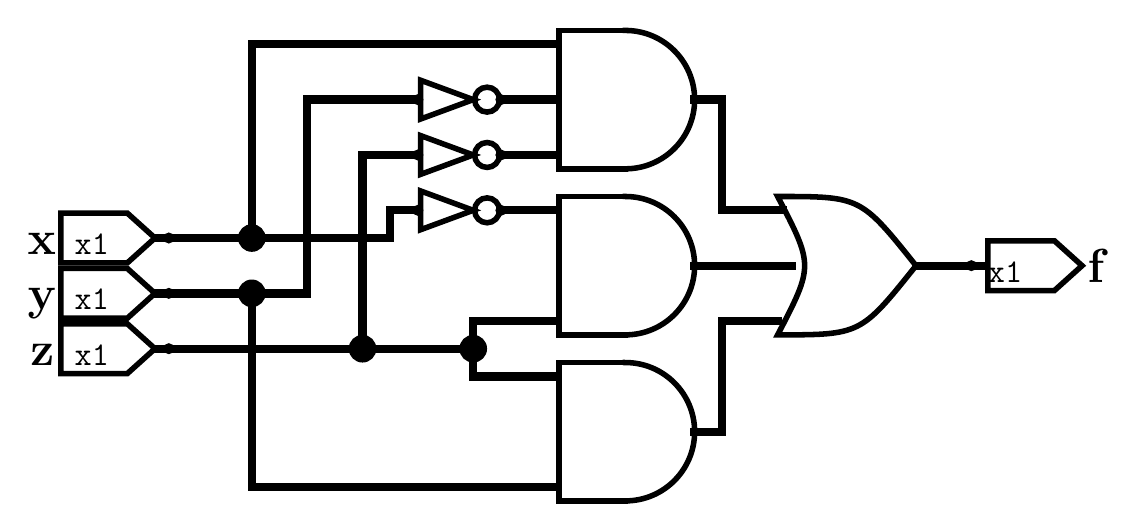
\begin{tikzpicture}[x=1pt,y=-1pt,line cap=rect]
\def\logisimfontA#1{\fontfamily{cmr}{#1}} % Replaced by logisim, original font was "SansSerif"
\def\logisimfontB#1{\fontfamily{cmtt}{#1}} % Replaced by logisim, original font was "Monospaced"
\definecolor{custcol_0_0_0}{RGB}{0, 0, 0}
\definecolor{custcol_ff_ff_ff}{RGB}{255, 255, 255}
\draw [line width=3.0pt, custcol_0_0_0 ]  (326.0,90.0) -- (346.0,90.0) ;
\draw [line width=3.0pt, custcol_0_0_0 ]  (196.0,10.0) -- (86.0,10.0) -- (86.0,80.0) -- (136.0,80.0) -- (136.0,70.0) -- (146.0,70.0) ;
\draw [line width=3.0pt, custcol_0_0_0 ]  (126.0,120.0) -- (166.0,120.0) ;
\draw [line width=3.0pt, custcol_0_0_0 ]  (196.0,110.0) -- (166.0,110.0) -- (166.0,120.0) -- (166.0,130.0) -- (196.0,130.0) ;
\draw [line width=3.0pt, custcol_0_0_0 ]  (176.0,50.0) -- (196.0,50.0) ;
\draw [line width=3.0pt, custcol_0_0_0 ]  (176.0,30.0) -- (196.0,30.0) ;
\draw [line width=3.0pt, custcol_0_0_0 ]  (176.0,70.0) -- (196.0,70.0) ;
\draw [line width=3.0pt, custcol_0_0_0 ]  (86.0,100.0) -- (106.0,100.0) -- (106.0,30.0) -- (146.0,30.0) ;
\fill [line width=3.0pt, custcol_0_0_0]  (166.0,120.0) ellipse (5.0 and 5.0 );
\fill [line width=3.0pt, custcol_0_0_0]  (126.0,120.0) ellipse (5.0 and 5.0 );
\fill [line width=3.0pt, custcol_0_0_0]  (86.0,80.0) ellipse (5.0 and 5.0 );
\fill [line width=3.0pt, custcol_0_0_0]  (86.0,100.0) ellipse (5.0 and 5.0 );
\draw [line width=3.0pt, custcol_0_0_0 ]  (350.0,90.0) -- (347.0,90.0) ;
\draw [line width=2.0pt, custcol_0_0_0 ]  (376.0,81.0) -- (386.0,90.0) -- (376.0,99.0) -- (352.0,99.0) -- (352.0,81.0) -- cycle;
\logisimfontB{\fontsize{12pt}{12pt}\selectfont\node[inner sep=0, outer sep=0, custcol_0_0_0, anchor=base west] at  (352.0,96.0)  {x1};}
\logisimfontA{\fontsize{16pt}{16pt}\fontseries{bx}\selectfont\node[inner sep=0, outer sep=0, custcol_0_0_0, anchor=base west] at  (388.0,96.0)  {f};}
\fill [line width=2.0pt, custcol_0_0_0]  (346.0,90.0) ellipse (2.0 and 2.0 );
\draw [line width=3.0pt, custcol_0_0_0 ]  (51.0,120.0) -- (56.0,120.0) -- (126.0,120.0) -- (126.0,50.0) -- (146.0,50.0) ;
\draw [line width=2.0pt, custcol_0_0_0 ]  (41.0,129.0) -- (51.0,120.0) -- (41.0,111.0) -- (17.0,111.0) -- (17.0,129.0) -- cycle;
\logisimfontB{\fontsize{12pt}{12pt}\selectfont\node[inner sep=0, outer sep=0, custcol_0_0_0, anchor=base west] at  (22.0,126.0)  {x1};}
\logisimfontA{\fontsize{16pt}{16pt}\fontseries{bx}\selectfont\node[inner sep=0, outer sep=0, custcol_0_0_0, anchor=base west] at  (6.0,126.0)  {z};}
\fill [line width=2.0pt, custcol_0_0_0]  (56.0,120.0) ellipse (2.0 and 2.0 );
\draw [line width=3.0pt, custcol_0_0_0 ]  (51.0,100.0) -- (56.0,100.0) -- (86.0,100.0) -- (86.0,170.0) -- (196.0,170.0) ;
\draw [line width=2.0pt, custcol_0_0_0 ]  (41.0,109.0) -- (51.0,100.0) -- (41.0,91.0) -- (17.0,91.0) -- (17.0,109.0) -- cycle;
\logisimfontB{\fontsize{12pt}{12pt}\selectfont\node[inner sep=0, outer sep=0, custcol_0_0_0, anchor=base west] at  (22.0,106.0)  {x1};}
\logisimfontA{\fontsize{16pt}{16pt}\fontseries{bx}\selectfont\node[inner sep=0, outer sep=0, custcol_0_0_0, anchor=base west] at  (5.0,106.0)  {y};}
\fill [line width=2.0pt, custcol_0_0_0]  (56.0,100.0) ellipse (2.0 and 2.0 );
\draw [line width=3.0pt, custcol_0_0_0 ]  (246.0,30.0) -- (256.0,30.0) -- (256.0,70.0) -- (276.0,70.0) -- (278.0,70.0) ;
\draw [line width=3.0pt, custcol_0_0_0 ]  (246.0,90.0) -- (276.0,90.0) -- (281.0,90.0) ;
\draw [line width=3.0pt, custcol_0_0_0 ]  (246.0,150.0) -- (256.0,150.0) -- (256.0,110.0) -- (276.0,110.0) -- (276.0,110.0) ;
\draw [line width=2.0pt, custcol_0_0_0 ]  (326.0,90.0) .. controls  (306.0,65.0)  ..  (276.0,65.0) .. controls  (289.0,90.0)  ..  (276.0,115.0) .. controls  (306.0,115.0)  ..  (326.0,90.0) -- cycle ;
\draw [line width=2.0pt, custcol_0_0_0 ]  (166.0,70.0) -- (147.0,63.0) -- (147.0,77.0) -- cycle;
\draw [line width=2.0pt, custcol_0_0_0]  (171.0,70.0) ellipse (4.5 and 4.5 );
\fill [line width=2.0pt, custcol_0_0_0]  (176.0,70.0) ellipse (2.0 and 2.0 );
\fill [line width=2.0pt, custcol_0_0_0]  (146.0,70.0) ellipse (2.0 and 2.0 );
\draw [line width=2.0pt, custcol_0_0_0] (221.0,115.0) arc (90.0:-90.0:25.0 and 25.0 );
\draw [line width=2.0pt, custcol_0_0_0 ]  (221.0,65.0) -- (197.0,65.0) -- (197.0,115.0) -- (221.0,115.0) ;
\draw [line width=2.0pt, custcol_0_0_0 ]  (166.0,30.0) -- (147.0,23.0) -- (147.0,37.0) -- cycle;
\draw [line width=2.0pt, custcol_0_0_0]  (171.0,30.0) ellipse (4.5 and 4.5 );
\fill [line width=2.0pt, custcol_0_0_0]  (176.0,30.0) ellipse (2.0 and 2.0 );
\fill [line width=2.0pt, custcol_0_0_0]  (146.0,30.0) ellipse (2.0 and 2.0 );
\draw [line width=2.0pt, custcol_0_0_0 ]  (166.0,50.0) -- (147.0,43.0) -- (147.0,57.0) -- cycle;
\draw [line width=2.0pt, custcol_0_0_0]  (171.0,50.0) ellipse (4.5 and 4.5 );
\fill [line width=2.0pt, custcol_0_0_0]  (176.0,50.0) ellipse (2.0 and 2.0 );
\fill [line width=2.0pt, custcol_0_0_0]  (146.0,50.0) ellipse (2.0 and 2.0 );
\draw [line width=3.0pt, custcol_0_0_0 ]  (51.0,80.0) -- (56.0,80.0) -- (86.0,80.0) ;
\draw [line width=2.0pt, custcol_0_0_0 ]  (41.0,89.0) -- (51.0,80.0) -- (41.0,71.0) -- (17.0,71.0) -- (17.0,89.0) -- cycle;
\logisimfontB{\fontsize{12pt}{12pt}\selectfont\node[inner sep=0, outer sep=0, custcol_0_0_0, anchor=base west] at  (22.0,86.0)  {x1};}
\logisimfontA{\fontsize{16pt}{16pt}\fontseries{bx}\selectfont\node[inner sep=0, outer sep=0, custcol_0_0_0, anchor=base west] at  (5.0,86.0)  {x};}
\fill [line width=2.0pt, custcol_0_0_0]  (56.0,80.0) ellipse (2.0 and 2.0 );
\draw [line width=2.0pt, custcol_0_0_0] (221.0,175.0) arc (90.0:-90.0:25.0 and 25.0 );
\draw [line width=2.0pt, custcol_0_0_0 ]  (221.0,125.0) -- (197.0,125.0) -- (197.0,175.0) -- (221.0,175.0) ;
\draw [line width=2.0pt, custcol_0_0_0] (221.0,55.0) arc (90.0:-90.0:25.0 and 25.0 );
\draw [line width=2.0pt, custcol_0_0_0 ]  (221.0,5.0) -- (197.0,5.0) -- (197.0,55.0) -- (221.0,55.0) ;
\end{tikzpicture}
}


				\label{fig:exe15}
			\end{figure}
			
	\end{columns}
\end{frame}

\begin{frame}{Mini prova 03}
	\begin{itemize}
		\item Dado o circuito abaixo, determine:
		\begin{enumerate}
			\item A tabela verdade correspondente ao circuito \textbf{não simplificado}.
			\item A expressão algébrica \textbf{simplificada} que representa a função lógica do circuito.
			\item O circuito simplificado.
			\item O diagrama de tempo (waveform) que reflete o comportamento do circuito.
		\end{enumerate}
	\end{itemize}
	\begin{figure}
		\centering
		% Important: If latex complains about unicode characters,
% please use "\usepackage[utf8x]{inputenc}" in your preamble
% You can change the size of the picture by putting it into the construct:
% 1) \resizebox{10cm}{!}{"below picture"} to scale horizontally to 10 cm
% 2) \resizebox{!}{15cm}{"below picture"} to scale vertically to 15 cm
% 3) \resizebox{10cm}{15cm}{"below picture"} a combination of above two
% It is not recomended to use the scale option of the tikzpicture environment.
\resizebox{10cm}{!}{
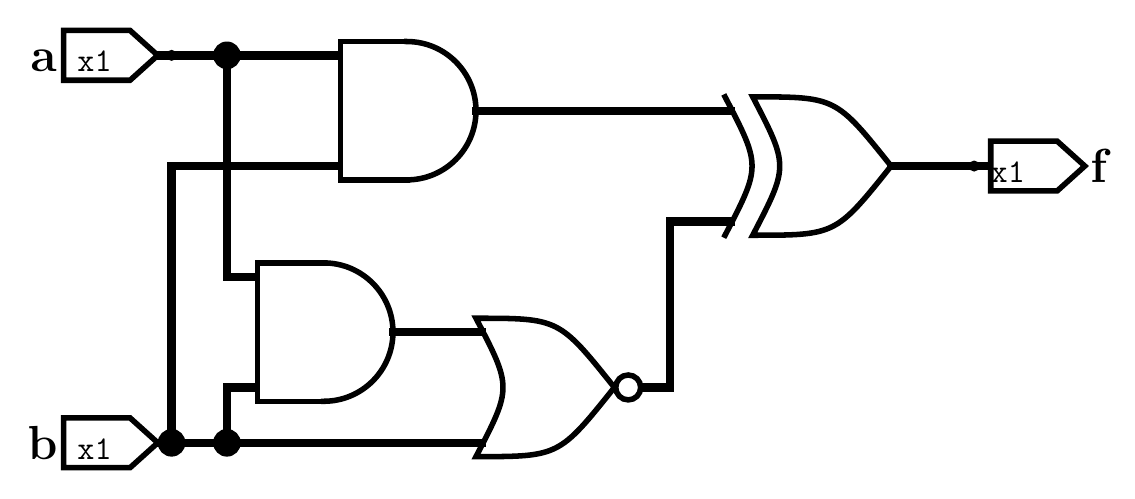
\begin{tikzpicture}[x=1pt,y=-1pt,line cap=rect]
\def\logisimfontA#1{\fontfamily{cmr}{#1}} % Replaced by logisim, original font was "SansSerif"
\def\logisimfontB#1{\fontfamily{cmtt}{#1}} % Replaced by logisim, original font was "Monospaced"
\definecolor{custcol_0_0_0}{RGB}{0, 0, 0}
\definecolor{custcol_ff_ff_ff}{RGB}{255, 255, 255}
\draw [line width=3.0pt, custcol_0_0_0 ]  (317.0,55.0) -- (347.0,55.0) ;
\draw [line width=3.0pt, custcol_0_0_0 ]  (117.0,55.0) -- (57.0,55.0) -- (57.0,155.0) -- (77.0,155.0) ;
\draw [line width=3.0pt, custcol_0_0_0 ]  (117.0,15.0) -- (77.0,15.0) -- (77.0,95.0) -- (87.0,95.0) ;
\fill [line width=3.0pt, custcol_0_0_0]  (57.0,155.0) ellipse (5.0 and 5.0 );
\fill [line width=3.0pt, custcol_0_0_0]  (77.0,15.0) ellipse (5.0 and 5.0 );
\fill [line width=3.0pt, custcol_0_0_0]  (77.0,155.0) ellipse (5.0 and 5.0 );
\draw [line width=3.0pt, custcol_0_0_0 ]  (52.0,155.0) -- (57.0,155.0) ;
\draw [line width=2.0pt, custcol_0_0_0 ]  (42.0,164.0) -- (52.0,155.0) -- (42.0,146.0) -- (18.0,146.0) -- (18.0,164.0) -- cycle;
\logisimfontB{\fontsize{12pt}{12pt}\selectfont\node[inner sep=0, outer sep=0, custcol_0_0_0, anchor=base west] at  (23.0,161.0)  {x1};}
\logisimfontA{\fontsize{16pt}{16pt}\fontseries{bx}\selectfont\node[inner sep=0, outer sep=0, custcol_0_0_0, anchor=base west] at  (5.0,161.0)  {b};}
\fill [line width=2.0pt, custcol_0_0_0]  (57.0,155.0) ellipse (2.0 and 2.0 );
\draw [line width=3.0pt, custcol_0_0_0 ]  (137.0,115.0) -- (167.0,115.0) -- (169.0,115.0) ;
\draw [line width=3.0pt, custcol_0_0_0 ]  (87.0,135.0) -- (77.0,135.0) -- (77.0,155.0) -- (167.0,155.0) -- (169.0,155.0) ;
\draw [line width=2.0pt, custcol_0_0_0 ]  (217.0,135.0) .. controls  (197.0,110.0)  ..  (167.0,110.0) .. controls  (180.0,135.0)  ..  (167.0,160.0) .. controls  (197.0,160.0)  ..  (217.0,135.0) -- cycle ;
\draw [line width=2.0pt, custcol_0_0_0]  (222.0,135.0) ellipse (4.5 and 4.5 );
\draw [line width=2.0pt, custcol_0_0_0] (112.0,140.0) arc (90.0:-90.0:25.0 and 25.0 );
\draw [line width=2.0pt, custcol_0_0_0 ]  (112.0,90.0) -- (88.0,90.0) -- (88.0,140.0) -- (112.0,140.0) ;
\draw [line width=3.0pt, custcol_0_0_0 ]  (52.0,15.0) -- (57.0,15.0) -- (77.0,15.0) ;
\draw [line width=2.0pt, custcol_0_0_0 ]  (42.0,24.0) -- (52.0,15.0) -- (42.0,6.0) -- (18.0,6.0) -- (18.0,24.0) -- cycle;
\logisimfontB{\fontsize{12pt}{12pt}\selectfont\node[inner sep=0, outer sep=0, custcol_0_0_0, anchor=base west] at  (23.0,21.0)  {x1};}
\logisimfontA{\fontsize{16pt}{16pt}\fontseries{bx}\selectfont\node[inner sep=0, outer sep=0, custcol_0_0_0, anchor=base west] at  (6.0,21.0)  {a};}
\fill [line width=2.0pt, custcol_0_0_0]  (57.0,15.0) ellipse (2.0 and 2.0 );
\draw [line width=3.0pt, custcol_0_0_0 ]  (167.0,35.0) -- (257.0,35.0) -- (259.0,35.0) ;
\draw [line width=3.0pt, custcol_0_0_0 ]  (227.0,135.0) -- (237.0,135.0) -- (237.0,75.0) -- (257.0,75.0) -- (259.0,75.0) ;
\draw [line width=2.0pt, custcol_0_0_0 ]  (317.0,55.0) .. controls  (297.0,30.0)  ..  (267.0,30.0) .. controls  (280.0,55.0)  ..  (267.0,80.0) .. controls  (297.0,80.0)  ..  (317.0,55.0) -- cycle ;
\draw [line width=2.0pt, custcol_0_0_0 ]  (257.0,30.0) .. controls  (270.0,55.0)  ..  (257.0,80.0) ;
\draw [line width=3.0pt, custcol_0_0_0 ]  (351.0,55.0) -- (348.0,55.0) ;
\draw [line width=2.0pt, custcol_0_0_0 ]  (377.0,46.0) -- (387.0,55.0) -- (377.0,64.0) -- (353.0,64.0) -- (353.0,46.0) -- cycle;
\logisimfontB{\fontsize{12pt}{12pt}\selectfont\node[inner sep=0, outer sep=0, custcol_0_0_0, anchor=base west] at  (353.0,61.0)  {x1};}
\logisimfontA{\fontsize{16pt}{16pt}\fontseries{bx}\selectfont\node[inner sep=0, outer sep=0, custcol_0_0_0, anchor=base west] at  (389.0,61.0)  {f};}
\fill [line width=2.0pt, custcol_0_0_0]  (347.0,55.0) ellipse (2.0 and 2.0 );
\draw [line width=2.0pt, custcol_0_0_0] (142.0,60.0) arc (90.0:-90.0:25.0 and 25.0 );
\draw [line width=2.0pt, custcol_0_0_0 ]  (142.0,10.0) -- (118.0,10.0) -- (118.0,60.0) -- (142.0,60.0) ;
\end{tikzpicture}
}

		\caption{Passarinho... Resolve esse... Qual é a expressão desse?\footnote[frame]{\textit{referência de velho}}}
		\label{fig:05exe}
	\end{figure}
\end{frame}

\section{\musEighth All you need is NAND/NOR... \musEighth}

\begin{frame}
	\frametitle{O que fazer se você não tem as portas lógicas que vc precisa}
	\par $\overline{a} = a\downarrow a = a \uparrow a$
	\begin{figure}
		\centering
		% Important: If latex complains about unicode characters,
% please use "\usepackage[utf8x]{inputenc}" in your preamble
% You can change the size of the picture by putting it into the construct:
% 1) \resizebox{10cm}{!}{"below picture"} to scale horizontally to 10 cm
% 2) \resizebox{!}{15cm}{"below picture"} to scale vertically to 15 cm
% 3) \resizebox{10cm}{15cm}{"below picture"} a combination of above two
% It is not recomended to use the scale option of the tikzpicture environment.
\resizebox{10cm}{!}{
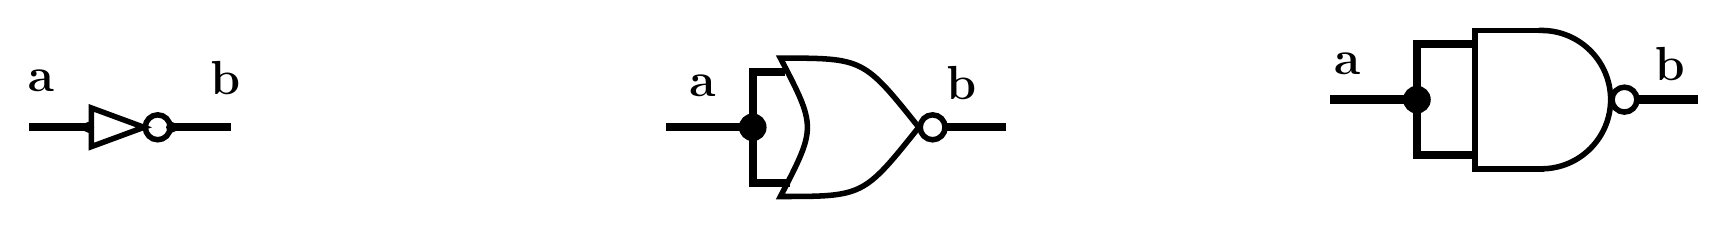
\begin{tikzpicture}[x=1pt,y=-1pt,line cap=rect]
\def\logisimfontA#1{\fontfamily{cmr}{#1}} % Replaced by logisim, original font was "SansSerif"
\definecolor{custcol_0_0_0}{RGB}{0, 0, 0}
\definecolor{custcol_ff_ff_ff}{RGB}{255, 255, 255}
\draw [line width=3.0pt, custcol_0_0_0 ]  (531.0,11.0) -- (511.0,11.0) -- (511.0,31.0) -- (511.0,51.0) -- (531.0,51.0) ;
\draw [line width=3.0pt, custcol_0_0_0 ]  (591.0,31.0) -- (611.0,31.0) ;
\draw [line width=3.0pt, custcol_0_0_0 ]  (241.0,41.0) -- (271.0,41.0) ;
\draw [line width=3.0pt, custcol_0_0_0 ]  (341.0,41.0) -- (361.0,41.0) ;
\draw [line width=3.0pt, custcol_0_0_0 ]  (481.0,31.0) -- (511.0,31.0) ;
\draw [line width=3.0pt, custcol_0_0_0 ]  (11.0,41.0) -- (31.0,41.0) ;
\draw [line width=3.0pt, custcol_0_0_0 ]  (61.0,41.0) -- (81.0,41.0) ;
\fill [line width=3.0pt, custcol_0_0_0]  (271.0,41.0) ellipse (5.0 and 5.0 );
\fill [line width=3.0pt, custcol_0_0_0]  (511.0,31.0) ellipse (5.0 and 5.0 );
\draw [line width=2.0pt, custcol_0_0_0 ]  (51.0,41.0) -- (32.0,34.0) -- (32.0,48.0) -- cycle;
\draw [line width=2.0pt, custcol_0_0_0]  (56.0,41.0) ellipse (4.5 and 4.5 );
\fill [line width=2.0pt, custcol_0_0_0]  (61.0,41.0) ellipse (2.0 and 2.0 );
\fill [line width=2.0pt, custcol_0_0_0]  (31.0,41.0) ellipse (2.0 and 2.0 );
\logisimfontA{\fontsize{16pt}{16pt}\fontseries{bx}\selectfont\node[inner sep=0, outer sep=0, custcol_0_0_0, anchor=base west] at  (75.0,29.0)  {b};}
\logisimfontA{\fontsize{16pt}{16pt}\fontseries{bx}\selectfont\node[inner sep=0, outer sep=0, custcol_0_0_0, anchor=base west] at  (597.0,24.0)  {b};}
\logisimfontA{\fontsize{16pt}{16pt}\fontseries{bx}\selectfont\node[inner sep=0, outer sep=0, custcol_0_0_0, anchor=base west] at  (341.0,31.0)  {b};}
\logisimfontA{\fontsize{16pt}{16pt}\fontseries{bx}\selectfont\node[inner sep=0, outer sep=0, custcol_0_0_0, anchor=base west] at  (248.0,30.0)  {a};}
\draw [line width=2.0pt, custcol_0_0_0] (556.0,56.0) arc (90.0:-90.0:25.0 and 25.0 );
\draw [line width=2.0pt, custcol_0_0_0 ]  (556.0,6.0) -- (532.0,6.0) -- (532.0,56.0) -- (556.0,56.0) ;
\draw [line width=2.0pt, custcol_0_0_0]  (586.0,31.0) ellipse (4.5 and 4.5 );
\logisimfontA{\fontsize{16pt}{16pt}\fontseries{bx}\selectfont\node[inner sep=0, outer sep=0, custcol_0_0_0, anchor=base west] at  (9.0,28.0)  {a};}
\logisimfontA{\fontsize{16pt}{16pt}\fontseries{bx}\selectfont\node[inner sep=0, outer sep=0, custcol_0_0_0, anchor=base west] at  (481.0,22.0)  {a};}
\draw [line width=3.0pt, custcol_0_0_0 ]  (281.0,21.0) -- (281.0,21.0) -- (271.0,21.0) -- (271.0,41.0) -- (271.0,61.0) -- (281.0,61.0) -- (283.0,61.0) ;
\draw [line width=2.0pt, custcol_0_0_0 ]  (331.0,41.0) .. controls  (311.0,16.0)  ..  (281.0,16.0) .. controls  (294.0,41.0)  ..  (281.0,66.0) .. controls  (311.0,66.0)  ..  (331.0,41.0) -- cycle ;
\draw [line width=2.0pt, custcol_0_0_0]  (336.0,41.0) ellipse (4.5 and 4.5 );
\end{tikzpicture}
}

		\label{fig:nandnot}
	\end{figure}
	
	\par $a.b = (a \downarrow a)\downarrow(b\downarrow b) = (a\uparrow b)\uparrow(a\uparrow b)$
	\begin{figure}
		\centering
		% Important: If latex complains about unicode characters,
% please use "\usepackage[utf8x]{inputenc}" in your preamble
% You can change the size of the picture by putting it into the construct:
% 1) \resizebox{10cm}{!}{"below picture"} to scale horizontally to 10 cm
% 2) \resizebox{!}{15cm}{"below picture"} to scale vertically to 15 cm
% 3) \resizebox{10cm}{15cm}{"below picture"} a combination of above two
% It is not recomended to use the scale option of the tikzpicture environment.
\resizebox{10cm}{!}{
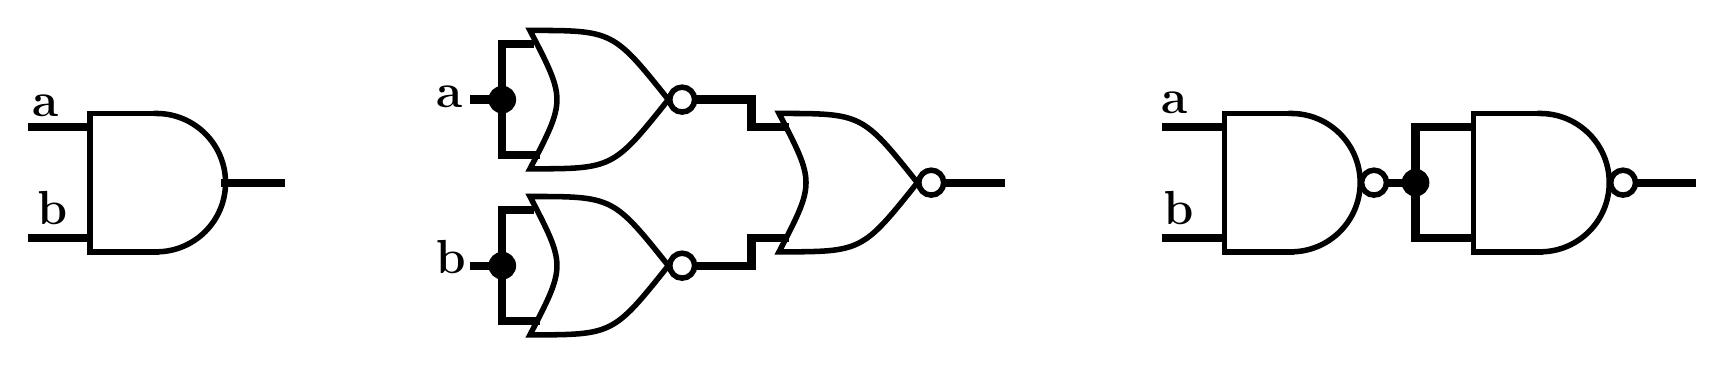
\begin{tikzpicture}[x=1pt,y=-1pt,line cap=rect]
\def\logisimfontA#1{\fontfamily{cmr}{#1}} % Replaced by logisim, original font was "SansSerif"
\definecolor{custcol_0_0_0}{RGB}{0, 0, 0}
\definecolor{custcol_ff_ff_ff}{RGB}{255, 255, 255}
\draw [line width=3.0pt, custcol_0_0_0 ]  (529.0,40.0) -- (509.0,40.0) -- (509.0,60.0) -- (509.0,80.0) -- (529.0,80.0) ;
\draw [line width=3.0pt, custcol_0_0_0 ]  (589.0,60.0) -- (609.0,60.0) ;
\draw [line width=3.0pt, custcol_0_0_0 ]  (339.0,60.0) -- (359.0,60.0) ;
\draw [line width=3.0pt, custcol_0_0_0 ]  (419.0,40.0) -- (439.0,40.0) ;
\draw [line width=3.0pt, custcol_0_0_0 ]  (419.0,80.0) -- (439.0,80.0) ;
\draw [line width=3.0pt, custcol_0_0_0 ]  (9.0,80.0) -- (29.0,80.0) ;
\draw [line width=3.0pt, custcol_0_0_0 ]  (9.0,40.0) -- (29.0,40.0) ;
\draw [line width=3.0pt, custcol_0_0_0 ]  (79.0,60.0) -- (99.0,60.0) ;
\draw [line width=3.0pt, custcol_0_0_0 ]  (169.0,90.0) -- (179.0,90.0) ;
\draw [line width=3.0pt, custcol_0_0_0 ]  (169.0,30.0) -- (179.0,30.0) ;
\draw [line width=3.0pt, custcol_0_0_0 ]  (499.0,60.0) -- (509.0,60.0) ;
\fill [line width=3.0pt, custcol_0_0_0]  (179.0,90.0) ellipse (5.0 and 5.0 );
\fill [line width=3.0pt, custcol_0_0_0]  (179.0,30.0) ellipse (5.0 and 5.0 );
\fill [line width=3.0pt, custcol_0_0_0]  (509.0,60.0) ellipse (5.0 and 5.0 );
\logisimfontA{\fontsize{16pt}{16pt}\fontseries{bx}\selectfont\node[inner sep=0, outer sep=0, custcol_0_0_0, anchor=base west] at  (155.0,93.0)  {b};}
\draw [line width=3.0pt, custcol_0_0_0 ]  (189.0,10.0) -- (189.0,10.0) -- (179.0,10.0) -- (179.0,30.0) -- (179.0,50.0) -- (189.0,50.0) -- (191.0,50.0) ;
\draw [line width=2.0pt, custcol_0_0_0 ]  (239.0,30.0) .. controls  (219.0,5.0)  ..  (189.0,5.0) .. controls  (202.0,30.0)  ..  (189.0,55.0) .. controls  (219.0,55.0)  ..  (239.0,30.0) -- cycle ;
\draw [line width=2.0pt, custcol_0_0_0]  (244.0,30.0) ellipse (4.5 and 4.5 );
\logisimfontA{\fontsize{16pt}{16pt}\fontseries{bx}\selectfont\node[inner sep=0, outer sep=0, custcol_0_0_0, anchor=base west] at  (418.0,75.0)  {b};}
\draw [line width=3.0pt, custcol_0_0_0 ]  (189.0,70.0) -- (189.0,70.0) -- (179.0,70.0) -- (179.0,90.0) -- (179.0,110.0) -- (189.0,110.0) -- (191.0,110.0) ;
\draw [line width=2.0pt, custcol_0_0_0 ]  (239.0,90.0) .. controls  (219.0,65.0)  ..  (189.0,65.0) .. controls  (202.0,90.0)  ..  (189.0,115.0) .. controls  (219.0,115.0)  ..  (239.0,90.0) -- cycle ;
\draw [line width=2.0pt, custcol_0_0_0]  (244.0,90.0) ellipse (4.5 and 4.5 );
\logisimfontA{\fontsize{16pt}{16pt}\fontseries{bx}\selectfont\node[inner sep=0, outer sep=0, custcol_0_0_0, anchor=base west] at  (11.0,75.0)  {b};}
\logisimfontA{\fontsize{16pt}{16pt}\fontseries{bx}\selectfont\node[inner sep=0, outer sep=0, custcol_0_0_0, anchor=base west] at  (417.0,35.0)  {a};}
\draw [line width=2.0pt, custcol_0_0_0] (554.0,85.0) arc (90.0:-90.0:25.0 and 25.0 );
\draw [line width=2.0pt, custcol_0_0_0 ]  (554.0,35.0) -- (530.0,35.0) -- (530.0,85.0) -- (554.0,85.0) ;
\draw [line width=2.0pt, custcol_0_0_0]  (584.0,60.0) ellipse (4.5 and 4.5 );
\draw [line width=2.0pt, custcol_0_0_0] (54.0,85.0) arc (90.0:-90.0:25.0 and 25.0 );
\draw [line width=2.0pt, custcol_0_0_0 ]  (54.0,35.0) -- (30.0,35.0) -- (30.0,85.0) -- (54.0,85.0) ;
\draw [line width=3.0pt, custcol_0_0_0 ]  (249.0,30.0) -- (269.0,30.0) -- (269.0,40.0) -- (279.0,40.0) -- (281.0,40.0) ;
\draw [line width=3.0pt, custcol_0_0_0 ]  (249.0,90.0) -- (269.0,90.0) -- (269.0,80.0) -- (279.0,80.0) -- (281.0,80.0) ;
\draw [line width=2.0pt, custcol_0_0_0 ]  (329.0,60.0) .. controls  (309.0,35.0)  ..  (279.0,35.0) .. controls  (292.0,60.0)  ..  (279.0,85.0) .. controls  (309.0,85.0)  ..  (329.0,60.0) -- cycle ;
\draw [line width=2.0pt, custcol_0_0_0]  (334.0,60.0) ellipse (4.5 and 4.5 );
\logisimfontA{\fontsize{16pt}{16pt}\fontseries{bx}\selectfont\node[inner sep=0, outer sep=0, custcol_0_0_0, anchor=base west] at  (155.0,33.0)  {a};}
\draw [line width=2.0pt, custcol_0_0_0] (464.0,85.0) arc (90.0:-90.0:25.0 and 25.0 );
\draw [line width=2.0pt, custcol_0_0_0 ]  (464.0,35.0) -- (440.0,35.0) -- (440.0,85.0) -- (464.0,85.0) ;
\draw [line width=2.0pt, custcol_0_0_0]  (494.0,60.0) ellipse (4.5 and 4.5 );
\logisimfontA{\fontsize{16pt}{16pt}\fontseries{bx}\selectfont\node[inner sep=0, outer sep=0, custcol_0_0_0, anchor=base west] at  (9.0,36.0)  {a};}
\end{tikzpicture}
}

		\label{fig:nandand}
	\end{figure}
	
	\par $a+b=(a \downarrow b)\downarrow(a \downarrow b)=(a \uparrow a)\uparrow(b \uparrow b)$
	\begin{figure}
		\centering
		% Important: If latex complains about unicode characters,
% please use "\usepackage[utf8x]{inputenc}" in your preamble
% You can change the size of the picture by putting it into the construct:
% 1) \resizebox{10cm}{!}{"below picture"} to scale horizontally to 10 cm
% 2) \resizebox{!}{15cm}{"below picture"} to scale vertically to 15 cm
% 3) \resizebox{10cm}{15cm}{"below picture"} a combination of above two
% It is not recomended to use the scale option of the tikzpicture environment.
\resizebox{10cm}{!}{
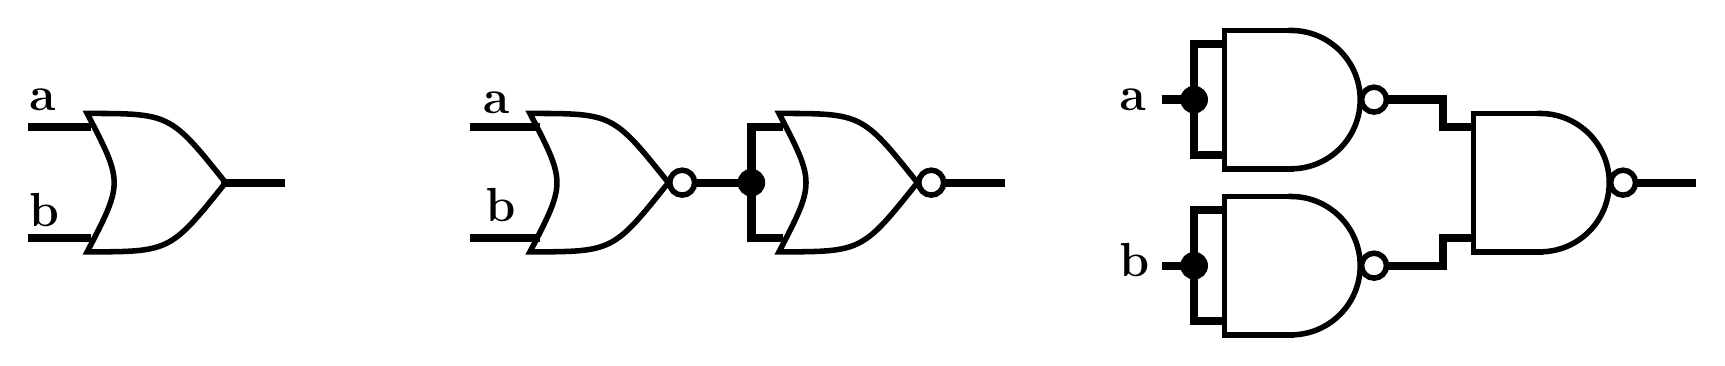
\begin{tikzpicture}[x=1pt,y=-1pt,line cap=rect]
\def\logisimfontA#1{\fontfamily{cmr}{#1}} % Replaced by logisim, original font was "SansSerif"
\definecolor{custcol_0_0_0}{RGB}{0, 0, 0}
\definecolor{custcol_ff_ff_ff}{RGB}{255, 255, 255}
\draw [line width=3.0pt, custcol_0_0_0 ]  (590.0,60.0) -- (610.0,60.0) ;
\draw [line width=3.0pt, custcol_0_0_0 ]  (250.0,60.0) -- (270.0,60.0) ;
\draw [line width=3.0pt, custcol_0_0_0 ]  (340.0,60.0) -- (360.0,60.0) ;
\draw [line width=3.0pt, custcol_0_0_0 ]  (80.0,60.0) -- (100.0,60.0) ;
\draw [line width=3.0pt, custcol_0_0_0 ]  (420.0,30.0) -- (430.0,30.0) ;
\draw [line width=3.0pt, custcol_0_0_0 ]  (440.0,10.0) -- (430.0,10.0) -- (430.0,30.0) -- (430.0,50.0) -- (440.0,50.0) ;
\draw [line width=3.0pt, custcol_0_0_0 ]  (420.0,90.0) -- (430.0,90.0) ;
\draw [line width=3.0pt, custcol_0_0_0 ]  (440.0,110.0) -- (430.0,110.0) -- (430.0,90.0) -- (430.0,70.0) -- (440.0,70.0) ;
\draw [line width=3.0pt, custcol_0_0_0 ]  (500.0,30.0) -- (520.0,30.0) -- (520.0,40.0) -- (530.0,40.0) ;
\draw [line width=3.0pt, custcol_0_0_0 ]  (500.0,90.0) -- (520.0,90.0) -- (520.0,80.0) -- (530.0,80.0) ;
\fill [line width=3.0pt, custcol_0_0_0]  (430.0,90.0) ellipse (5.0 and 5.0 );
\fill [line width=3.0pt, custcol_0_0_0]  (270.0,60.0) ellipse (5.0 and 5.0 );
\fill [line width=3.0pt, custcol_0_0_0]  (430.0,30.0) ellipse (5.0 and 5.0 );
\draw [line width=3.0pt, custcol_0_0_0 ]  (170.0,40.0) -- (190.0,40.0) -- (192.0,40.0) ;
\draw [line width=3.0pt, custcol_0_0_0 ]  (170.0,80.0) -- (190.0,80.0) -- (192.0,80.0) ;
\draw [line width=2.0pt, custcol_0_0_0 ]  (240.0,60.0) .. controls  (220.0,35.0)  ..  (190.0,35.0) .. controls  (203.0,60.0)  ..  (190.0,85.0) .. controls  (220.0,85.0)  ..  (240.0,60.0) -- cycle ;
\draw [line width=2.0pt, custcol_0_0_0]  (245.0,60.0) ellipse (4.5 and 4.5 );
\draw [line width=3.0pt, custcol_0_0_0 ]  (280.0,40.0) -- (280.0,40.0) -- (270.0,40.0) -- (270.0,60.0) -- (270.0,80.0) -- (280.0,80.0) -- (280.0,80.0) ;
\draw [line width=2.0pt, custcol_0_0_0 ]  (330.0,60.0) .. controls  (310.0,35.0)  ..  (280.0,35.0) .. controls  (293.0,60.0)  ..  (280.0,85.0) .. controls  (310.0,85.0)  ..  (330.0,60.0) -- cycle ;
\draw [line width=2.0pt, custcol_0_0_0]  (335.0,60.0) ellipse (4.5 and 4.5 );
\logisimfontA{\fontsize{16pt}{16pt}\fontseries{bx}\selectfont\node[inner sep=0, outer sep=0, custcol_0_0_0, anchor=base west] at  (9.0,34.0)  {a};}
\draw [line width=2.0pt, custcol_0_0_0] (555.0,85.0) arc (90.0:-90.0:25.0 and 25.0 );
\draw [line width=2.0pt, custcol_0_0_0 ]  (555.0,35.0) -- (531.0,35.0) -- (531.0,85.0) -- (555.0,85.0) ;
\draw [line width=2.0pt, custcol_0_0_0]  (585.0,60.0) ellipse (4.5 and 4.5 );
\logisimfontA{\fontsize{16pt}{16pt}\fontseries{bx}\selectfont\node[inner sep=0, outer sep=0, custcol_0_0_0, anchor=base west] at  (9.0,76.0)  {b};}
\logisimfontA{\fontsize{16pt}{16pt}\fontseries{bx}\selectfont\node[inner sep=0, outer sep=0, custcol_0_0_0, anchor=base west] at  (403.0,94.0)  {b};}
\logisimfontA{\fontsize{16pt}{16pt}\fontseries{bx}\selectfont\node[inner sep=0, outer sep=0, custcol_0_0_0, anchor=base west] at  (174.0,74.0)  {b};}
\logisimfontA{\fontsize{16pt}{16pt}\fontseries{bx}\selectfont\node[inner sep=0, outer sep=0, custcol_0_0_0, anchor=base west] at  (403.0,34.0)  {a};}
\draw [line width=2.0pt, custcol_0_0_0] (465.0,115.0) arc (90.0:-90.0:25.0 and 25.0 );
\draw [line width=2.0pt, custcol_0_0_0 ]  (465.0,65.0) -- (441.0,65.0) -- (441.0,115.0) -- (465.0,115.0) ;
\draw [line width=2.0pt, custcol_0_0_0]  (495.0,90.0) ellipse (4.5 and 4.5 );
\draw [line width=3.0pt, custcol_0_0_0 ]  (10.0,40.0) -- (30.0,40.0) -- (30.0,40.0) ;
\draw [line width=3.0pt, custcol_0_0_0 ]  (10.0,80.0) -- (30.0,80.0) -- (30.0,80.0) ;
\draw [line width=2.0pt, custcol_0_0_0 ]  (80.0,60.0) .. controls  (60.0,35.0)  ..  (30.0,35.0) .. controls  (43.0,60.0)  ..  (30.0,85.0) .. controls  (60.0,85.0)  ..  (80.0,60.0) -- cycle ;
\logisimfontA{\fontsize{16pt}{16pt}\fontseries{bx}\selectfont\node[inner sep=0, outer sep=0, custcol_0_0_0, anchor=base west] at  (173.0,35.0)  {a};}
\draw [line width=2.0pt, custcol_0_0_0] (465.0,55.0) arc (90.0:-90.0:25.0 and 25.0 );
\draw [line width=2.0pt, custcol_0_0_0 ]  (465.0,5.0) -- (441.0,5.0) -- (441.0,55.0) -- (465.0,55.0) ;
\draw [line width=2.0pt, custcol_0_0_0]  (495.0,30.0) ellipse (4.5 and 4.5 );
\end{tikzpicture}
}

		\label{fig:nandor}
	\end{figure}
\end{frame}

\section{O que mídia não quer que você saiba sobre o XOR \footnote[frame]{Coringando já...}}

\begin{frame}
	\frametitle{Equivalências do XOR}
	\par Até agora nos foram apresentadas as equivalências das portas AND e OR, porém, muitas vezes nos depararemos com portas XOR. Seria interessante sabermos sua equivalências também:
	
	\begin{table}[h!]
		\centering
		\begin{tabular}{|c|c|c|c|c|c|c|c|c|c|c|}
			\hline
			a & b & \(a \oplus b\) & \(\overline{a}b + a\overline{b}\) & \(\overline{\overline{a}\overline{b} + ab}\) & \(\overline{a}\) & \(\overline{b}\) & \(ab\) & \(\overline{a}b\) & \(a\overline{b}\) & \(\overline{a}\overline{b}\) \\ \hline
			0 & 0 & 0 & 0 & 0 & 1 & 1 & 0 & 0 & 0 & 1 \\ \hline
			0 & 1 & 1 & 1 & 1 & 1 & 0 & 0 & 1 & 0 & 0 \\ \hline
			1 & 0 & 1 & 1 & 1 & 0 & 1 & 0 & 0 & 1 & 0 \\ \hline
			1 & 1 & 0 & 0 & 0 & 0 & 0 & 1 & 0 & 0 & 0 \\ \hline
		\end{tabular}
		\caption{Tabela verdade das equivalências de XOR}
		\label{tab:equivalXOR}
	\end{table}
	
	\par $a \oplus b = \overline{a}b + a\overline{b}\ = \overline{\overline{a}\overline{b} + ab}$
	
\end{frame}

\begin{frame}
	\frametitle{Equivalências do XOR - Exercício}
	\par Usando a tabela verdade prove que $a \oplus (b \oplus c) = (a \oplus b) \oplus c$ e portanto que XOR é comutativo.
\end{frame}

\begin{frame}
	\frametitle{Revelação!}
	\par Que idade você tinha ao ficar sabendo que XOR só tem saída verdadeira quando o número de entradas verdadeiras é ímpar??
\end{frame}
















	\section{Bom... Agora vamos fazer algumas coisa legais: \\Somadores e subtratores.}
		\subsection{Somadores}
\begin{frame}
	\frametitle{Como fazer a soma binária}
	\framesubtitle{Expressão de exemplo}
	\par Abaixo foi realizada uma operação de soma simples entre dois números binários, a e b, cujo resultado é mostrado na linha marcada com a palavra 'Sum'. '$C_{in}$' e '$C_{out}$' significa 'Carry in' e 'Carry out', o nosso famoso 'Vai um'. A partir deste exemplo, vamos criar uma tabela-verdade que nos permitirá formular a expressão algébrica booleana e, consequentemente, o circuito somador correspondente.
	
	\begin{table}[h!]
		\centering
		\begin{tabular}{cccc>{\centering\arraybackslash}p{2cm}}
		  $\overset{C_{out}}{1}$ & $\overset{C_{in}}{1}$ & & & $C_{in}$ / $C_{out}$ \\ \cline{1-4}
			& 1 & 1 & 0 & a \\ 
			& 1 & 1 & 1 & b \\ \cline{1-4}
			1 & 1 & 0 & 1 & Sum \\
		\end{tabular}
	\end{table}
	
\end{frame}

\begin{frame}
	\frametitle{Como fazer a soma binária}
	\only<1>{
		\framesubtitle{Tabela verdade da soma}
		\par Abaixo, representamos a tabela-verdade da soma binária. O objetivo da desta é modelar o comportamento da soma de dois bits. Como vimos na soma binária anterior, quando um bit 1 é somado a outro bit 1, o valor resultante é zero; no entanto, a próxima soma recebe um bit 1 adicional. Esse bit adicional é chamado de 'Carry in' quando é recebido, e de 'Carry out' quando é emitido. O objetivo da tabela-verdade abaixo é representar a soma e o 'Carry out' resultantes da soma de dois bits.
		\begin{table}[h!]
			\centering
			\begin{tabular}{|c|c|c|c|}
				\hline
				a & b & Sum & $C_{out}$\\ \hline
				0 & 0 & 0   & 0          \\ \hline
				0 & 1 & 1   & 0          \\ \hline
				1 & 0 & 1   & 0          \\ \hline
				1 & 1 & 0   & 1          \\ \hline
			\end{tabular}
			\caption{Tabela verdade da soma binária}
			\label{tab:binary_addition}
		\end{table}
		
	}
	\only<2>{
		\framesubtitle{\textbf{Prática dirigida} - Tabela verdade da soma}
		\par Como $Sum$ e $C_{out}$ se comportam? O que $C_{out}$ representa em termos de uma soma computacional? Qual o circuito correspondente?
		\begin{table}[h!]
			\centering
			\begin{tabular}{|c|c|c|c|}
				\hline
				a & b & Sum & $C_{out}$\\ \hline
				0 & 0 & 0   & 0          \\ \hline
				0 & 1 & 1   & 0          \\ \hline
				1 & 0 & 1   & 0          \\ \hline
				1 & 1 & 0   & 1          \\ \hline
			\end{tabular}
			\caption{Tabela verdade da soma binária}
			\label{tab:binary_addition2}
		\end{table}
	}
	\only<3>{
		\framesubtitle{\textbf{Prática dirigida} - Tabela verdade da soma}
		\begin{columns}
			\column{.5\linewidth}
			\begin{table}[h!]
				\centering
				\begin{tabular}{|c|c|c|c|c|c|}
					\hline
					a & b & Sum & \(C_{out}\)& \(a \oplus b\) & \(a \cdot b\) \\ \hline
					0 & 0 & 0   & 0          & 0              & 0             \\ \hline
					0 & 1 & 1   & 0          & 1              & 0             \\ \hline
					1 & 0 & 1   & 0          & 1              & 0             \\ \hline
					1 & 1 & 0   & 1          & 0              & 1             \\ \hline
				\end{tabular}
				\caption{Tabela verdade da soma binária}
				\label{tab:binary_addition3}
			\end{table}
			\column{.5\linewidth}
			\begin{figure}
				\centering
				% Important: If latex complains about unicode characters,
% please use "\usepackage[utf8x]{inputenc}" in your preamble
% You can change the size of the picture by putting it into the construct:
% 1) \resizebox{10cm}{!}{"below picture"} to scale horizontally to 10 cm
% 2) \resizebox{!}{15cm}{"below picture"} to scale vertically to 15 cm
% 3) \resizebox{10cm}{15cm}{"below picture"} a combination of above two
% It is not recomended to use the scale option of the tikzpicture environment.
\resizebox{\linewidth}{!}{
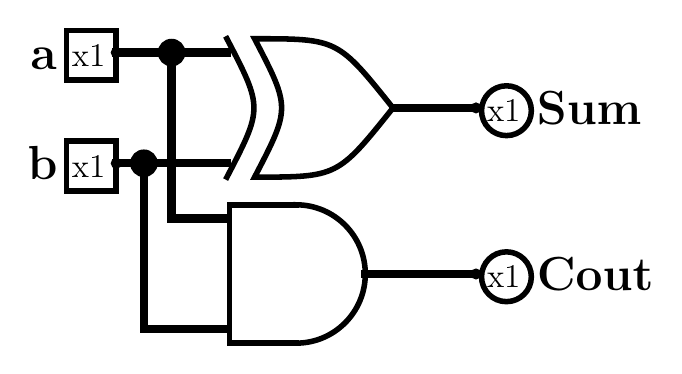
\begin{tikzpicture}[x=1pt,y=-1pt,line cap=rect]
\def\logisimfontA#1{\fontfamily{cmr}{#1}} % Replaced by logisim, original font was "SansSerif"
\definecolor{custcol_0_0_0}{RGB}{0, 0, 0}
\definecolor{custcol_ff_ff_ff}{RGB}{255, 255, 255}
\draw [line width=3.0pt, custcol_0_0_0 ]  (137.0,35.0) -- (167.0,35.0) ;
\draw [line width=3.0pt, custcol_0_0_0 ]  (127.0,95.0) -- (167.0,95.0) ;
\draw [line width=3.0pt, custcol_0_0_0 ]  (37.0,15.0) -- (57.0,15.0) -- (57.0,75.0) -- (77.0,75.0) ;
\draw [line width=3.0pt, custcol_0_0_0 ]  (47.0,55.0) -- (47.0,115.0) -- (77.0,115.0) ;
\fill [line width=3.0pt, custcol_0_0_0]  (47.0,55.0) ellipse (5.0 and 5.0 );
\fill [line width=3.0pt, custcol_0_0_0]  (57.0,15.0) ellipse (5.0 and 5.0 );
\draw [line width=2.0pt, custcol_0_0_0 ]  (19.0,7.0) -- (36.0,7.0) ;
\draw [line width=2.0pt, custcol_0_0_0 ]  (37.0,7.0) -- (37.0,24.0) ;
\draw [line width=2.0pt, custcol_0_0_0 ]  (37.0,25.0) -- (20.0,25.0) ;
\draw [line width=2.0pt, custcol_0_0_0 ]  (19.0,25.0) -- (19.0,8.0) ;
\logisimfontA{\fontsize{12pt}{12pt}\selectfont\node[inner sep=0, outer sep=0, custcol_0_0_0, anchor=base west] at  (21.0,20.0)  {x1};}
\logisimfontA{\fontsize{16pt}{16pt}\fontseries{bx}\selectfont\node[inner sep=0, outer sep=0, custcol_0_0_0, anchor=base west] at  (6.0,21.0)  {a};}
\fill [line width=2.0pt, custcol_0_0_0]  (37.0,15.0) ellipse (2.0 and 2.0 );
\draw [line width=2.0pt, custcol_0_0_0 ]  (19.0,47.0) -- (36.0,47.0) ;
\draw [line width=2.0pt, custcol_0_0_0 ]  (37.0,47.0) -- (37.0,64.0) ;
\draw [line width=2.0pt, custcol_0_0_0 ]  (37.0,65.0) -- (20.0,65.0) ;
\draw [line width=2.0pt, custcol_0_0_0 ]  (19.0,65.0) -- (19.0,48.0) ;
\logisimfontA{\fontsize{12pt}{12pt}\selectfont\node[inner sep=0, outer sep=0, custcol_0_0_0, anchor=base west] at  (21.0,60.0)  {x1};}
\logisimfontA{\fontsize{16pt}{16pt}\fontseries{bx}\selectfont\node[inner sep=0, outer sep=0, custcol_0_0_0, anchor=base west] at  (5.0,61.0)  {b};}
\fill [line width=2.0pt, custcol_0_0_0]  (37.0,55.0) ellipse (2.0 and 2.0 );
\draw [line width=2.0pt, custcol_0_0_0]  (178.0,96.0) ellipse (9.0 and 9.0 );
\logisimfontA{\fontsize{12pt}{12pt}\selectfont\node[inner sep=0, outer sep=0, custcol_0_0_0, anchor=base west] at  (171.0,100.0)  {x1};}
\logisimfontA{\fontsize{16pt}{16pt}\fontseries{bx}\selectfont\node[inner sep=0, outer sep=0, custcol_0_0_0, anchor=base west] at  (189.0,101.0)  {Cout};}
\fill [line width=2.0pt, custcol_0_0_0]  (167.0,95.0) ellipse (2.0 and 2.0 );
\draw [line width=2.0pt, custcol_0_0_0] (102.0,120.0) arc (90.0:-90.0:25.0 and 25.0 );
\draw [line width=2.0pt, custcol_0_0_0 ]  (102.0,70.0) -- (78.0,70.0) -- (78.0,120.0) -- (102.0,120.0) ;
\draw [line width=3.0pt, custcol_0_0_0 ]  (57.0,15.0) -- (77.0,15.0) -- (77.0,15.0) ;
\draw [line width=3.0pt, custcol_0_0_0 ]  (37.0,55.0) -- (47.0,55.0) -- (77.0,55.0) -- (77.0,55.0) ;
\draw [line width=2.0pt, custcol_0_0_0 ]  (137.0,35.0) .. controls  (117.0,10.0)  ..  (87.0,10.0) .. controls  (100.0,35.0)  ..  (87.0,60.0) .. controls  (117.0,60.0)  ..  (137.0,35.0) -- cycle ;
\draw [line width=2.0pt, custcol_0_0_0 ]  (77.0,10.0) .. controls  (90.0,35.0)  ..  (77.0,60.0) ;
\draw [line width=2.0pt, custcol_0_0_0]  (178.0,36.0) ellipse (9.0 and 9.0 );
\logisimfontA{\fontsize{12pt}{12pt}\selectfont\node[inner sep=0, outer sep=0, custcol_0_0_0, anchor=base west] at  (171.0,40.0)  {x1};}
\logisimfontA{\fontsize{16pt}{16pt}\fontseries{bx}\selectfont\node[inner sep=0, outer sep=0, custcol_0_0_0, anchor=base west] at  (189.0,41.0)  {Sum};}
\fill [line width=2.0pt, custcol_0_0_0]  (167.0,35.0) ellipse (2.0 and 2.0 );
\end{tikzpicture}
}

				\label{fig:somadorincompleto}
			\end{figure}
			
		\end{columns}
	}
\end{frame}
\begin{frame}
	\frametitle{Meio somador / Somador incompleto / Half adder}
	\par A tabela-verdade e o circuito mostrados abaixo representam o que chamamos de \textbf{meio somador}, \textbf{somador incompleto} ou ainda \textit{\textbf{Half Adder}}. O meio somador tem essa denominação porque, apesar de realizar a soma de dois bits, não considera um bit que possa vir para complementar sua operação. Dessa forma, o circuito é capaz de trabalhar apenas com a soma de dois bits, informando se houve um bit $C_{out}$. Isso impede a criação de somadores para números maiores por meio da concatenação de vários circuitos
	\begin{columns}
		\column{.5\linewidth}
		\begin{table}[h!]
			\centering
			\begin{tabular}{|c|c|c|c|c|c|}
				\hline
				a & b & Sum & \(C_{out}\)& \(a \oplus b\) & \(a \cdot b\) \\ \hline
				0 & 0 & 0   & 0          & 0              & 0             \\ \hline
				0 & 1 & 1   & 0          & 1              & 0             \\ \hline
				1 & 0 & 1   & 0          & 1              & 0             \\ \hline
				1 & 1 & 0   & 1          & 0              & 1             \\ \hline
			\end{tabular}
			\caption{Tabela verdade da soma binária}
			\label{tab:binary_addition4}
		\end{table}
		\column{.5\linewidth}
		\begin{figure}
			\centering
			% Important: If latex complains about unicode characters,
% please use "\usepackage[utf8x]{inputenc}" in your preamble
% You can change the size of the picture by putting it into the construct:
% 1) \resizebox{10cm}{!}{"below picture"} to scale horizontally to 10 cm
% 2) \resizebox{!}{15cm}{"below picture"} to scale vertically to 15 cm
% 3) \resizebox{10cm}{15cm}{"below picture"} a combination of above two
% It is not recomended to use the scale option of the tikzpicture environment.
\resizebox{\linewidth}{!}{
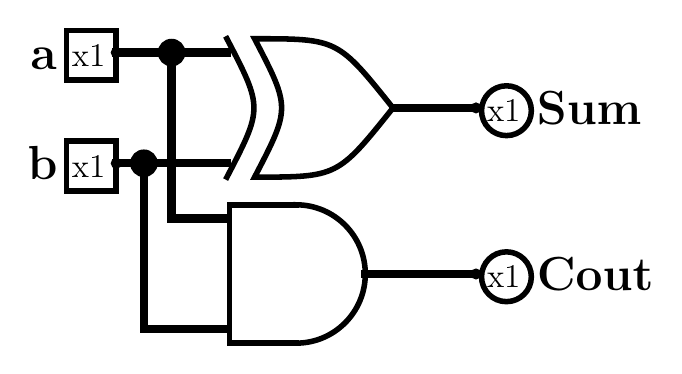
\begin{tikzpicture}[x=1pt,y=-1pt,line cap=rect]
\def\logisimfontA#1{\fontfamily{cmr}{#1}} % Replaced by logisim, original font was "SansSerif"
\definecolor{custcol_0_0_0}{RGB}{0, 0, 0}
\definecolor{custcol_ff_ff_ff}{RGB}{255, 255, 255}
\draw [line width=3.0pt, custcol_0_0_0 ]  (137.0,35.0) -- (167.0,35.0) ;
\draw [line width=3.0pt, custcol_0_0_0 ]  (127.0,95.0) -- (167.0,95.0) ;
\draw [line width=3.0pt, custcol_0_0_0 ]  (37.0,15.0) -- (57.0,15.0) -- (57.0,75.0) -- (77.0,75.0) ;
\draw [line width=3.0pt, custcol_0_0_0 ]  (47.0,55.0) -- (47.0,115.0) -- (77.0,115.0) ;
\fill [line width=3.0pt, custcol_0_0_0]  (47.0,55.0) ellipse (5.0 and 5.0 );
\fill [line width=3.0pt, custcol_0_0_0]  (57.0,15.0) ellipse (5.0 and 5.0 );
\draw [line width=2.0pt, custcol_0_0_0 ]  (19.0,7.0) -- (36.0,7.0) ;
\draw [line width=2.0pt, custcol_0_0_0 ]  (37.0,7.0) -- (37.0,24.0) ;
\draw [line width=2.0pt, custcol_0_0_0 ]  (37.0,25.0) -- (20.0,25.0) ;
\draw [line width=2.0pt, custcol_0_0_0 ]  (19.0,25.0) -- (19.0,8.0) ;
\logisimfontA{\fontsize{12pt}{12pt}\selectfont\node[inner sep=0, outer sep=0, custcol_0_0_0, anchor=base west] at  (21.0,20.0)  {x1};}
\logisimfontA{\fontsize{16pt}{16pt}\fontseries{bx}\selectfont\node[inner sep=0, outer sep=0, custcol_0_0_0, anchor=base west] at  (6.0,21.0)  {a};}
\fill [line width=2.0pt, custcol_0_0_0]  (37.0,15.0) ellipse (2.0 and 2.0 );
\draw [line width=2.0pt, custcol_0_0_0 ]  (19.0,47.0) -- (36.0,47.0) ;
\draw [line width=2.0pt, custcol_0_0_0 ]  (37.0,47.0) -- (37.0,64.0) ;
\draw [line width=2.0pt, custcol_0_0_0 ]  (37.0,65.0) -- (20.0,65.0) ;
\draw [line width=2.0pt, custcol_0_0_0 ]  (19.0,65.0) -- (19.0,48.0) ;
\logisimfontA{\fontsize{12pt}{12pt}\selectfont\node[inner sep=0, outer sep=0, custcol_0_0_0, anchor=base west] at  (21.0,60.0)  {x1};}
\logisimfontA{\fontsize{16pt}{16pt}\fontseries{bx}\selectfont\node[inner sep=0, outer sep=0, custcol_0_0_0, anchor=base west] at  (5.0,61.0)  {b};}
\fill [line width=2.0pt, custcol_0_0_0]  (37.0,55.0) ellipse (2.0 and 2.0 );
\draw [line width=2.0pt, custcol_0_0_0]  (178.0,96.0) ellipse (9.0 and 9.0 );
\logisimfontA{\fontsize{12pt}{12pt}\selectfont\node[inner sep=0, outer sep=0, custcol_0_0_0, anchor=base west] at  (171.0,100.0)  {x1};}
\logisimfontA{\fontsize{16pt}{16pt}\fontseries{bx}\selectfont\node[inner sep=0, outer sep=0, custcol_0_0_0, anchor=base west] at  (189.0,101.0)  {Cout};}
\fill [line width=2.0pt, custcol_0_0_0]  (167.0,95.0) ellipse (2.0 and 2.0 );
\draw [line width=2.0pt, custcol_0_0_0] (102.0,120.0) arc (90.0:-90.0:25.0 and 25.0 );
\draw [line width=2.0pt, custcol_0_0_0 ]  (102.0,70.0) -- (78.0,70.0) -- (78.0,120.0) -- (102.0,120.0) ;
\draw [line width=3.0pt, custcol_0_0_0 ]  (57.0,15.0) -- (77.0,15.0) -- (77.0,15.0) ;
\draw [line width=3.0pt, custcol_0_0_0 ]  (37.0,55.0) -- (47.0,55.0) -- (77.0,55.0) -- (77.0,55.0) ;
\draw [line width=2.0pt, custcol_0_0_0 ]  (137.0,35.0) .. controls  (117.0,10.0)  ..  (87.0,10.0) .. controls  (100.0,35.0)  ..  (87.0,60.0) .. controls  (117.0,60.0)  ..  (137.0,35.0) -- cycle ;
\draw [line width=2.0pt, custcol_0_0_0 ]  (77.0,10.0) .. controls  (90.0,35.0)  ..  (77.0,60.0) ;
\draw [line width=2.0pt, custcol_0_0_0]  (178.0,36.0) ellipse (9.0 and 9.0 );
\logisimfontA{\fontsize{12pt}{12pt}\selectfont\node[inner sep=0, outer sep=0, custcol_0_0_0, anchor=base west] at  (171.0,40.0)  {x1};}
\logisimfontA{\fontsize{16pt}{16pt}\fontseries{bx}\selectfont\node[inner sep=0, outer sep=0, custcol_0_0_0, anchor=base west] at  (189.0,41.0)  {Sum};}
\fill [line width=2.0pt, custcol_0_0_0]  (167.0,35.0) ellipse (2.0 and 2.0 );
\end{tikzpicture}
}

			\label{fig:somadorincompleto2}
		\end{figure}
		
	\end{columns}
\end{frame}
\begin{frame}
	\frametitle{Somador completo}
	\par Para determinar um somador completo, é necessário considerar não apenas as entradas $a$ e $b$, mas também uma entrada $C_{in}$​, que representa o possível bit vindo do $C_{out}$​ de outro circuito. Dessa forma, o resultado da soma é alterado, o que, por sua vez, modifica a expressão final e o circuito resultante.
	\begin{table}[h!]
		\centering
		\begin{tabular}{|c|c|c|c|}
			\hline
			a & b & $C_{in}$ & Sum \\
			\hline
			0 & 0 & 0 & 0 \\
			0 & 0 & 1 & 1 \\
			0 & 1 & 0 & 1 \\
			0 & 1 & 1 & 0 \\
			1 & 0 & 0 & 1 \\
			1 & 0 & 1 & 0 \\
			1 & 1 & 0 & 0 \\
			1 & 1 & 1 & 1 \\
			\hline
		\end{tabular}
		\caption{Tabela verdade de um somador completo}
		\label{tab:full_adder}
	\end{table}
\end{frame}

\begin{frame}
	\frametitle{Somador completo}
	\framesubtitle{\textbf{Prática guiada}}
	\par Considerando a tabela verdade mostrada determine a expressão algébrica boleana e o circuito correspondentes.
	\begin{columns}
		\column{.5\linewidth}
			\begin{table}[h!]
				\centering
				\begin{tabular}{|c|c|c|c|}
					\hline
					a & b & $C_{in}$ & Sum \\
					\hline
					0 & 0 & 0 & 0 \\
					0 & 0 & 1 & 1 \\
					0 & 1 & 0 & 1 \\
					0 & 1 & 1 & 0 \\
					1 & 0 & 0 & 1 \\
					1 & 0 & 1 & 0 \\
					1 & 1 & 0 & 0 \\
					1 & 1 & 1 & 1 \\
					\hline
				\end{tabular}
				\caption{Tabela verdade de $C_{in}$ para somador completo}
				\label{tab:full_adder2}
			\end{table}
		\column{.5\linewidth}
			\pause
			\par Para facilitar a notação considerando $c=C_{in}$ Temos por \textit{mimtermos}:
			\begin{equation}
				\begin{aligned}
					&(\overline{a}\overline{b}c)+(\overline{a}b\overline{c})+(a\overline{b}\overline{c})+(abc) = \\
					&\overline{a}.(\overline{b}c+b\overline{c}) + a.(\overline{b}\overline{c}+bc) = \\
					&\overline{a}.(b \oplus c) + a.(\overline{b \oplus c}) = \\
					& \boxed{a \oplus (b \oplus c)}
				\end{aligned}
			\end{equation}
			\vspace{-0.5cm}
			\pause
			\begin{figure}
				\centering
				% Important: If latex complains about unicode characters,
% please use "\usepackage[utf8x]{inputenc}" in your preamble
% You can change the size of the picture by putting it into the construct:
% 1) \resizebox{10cm}{!}{"below picture"} to scale horizontally to 10 cm
% 2) \resizebox{!}{15cm}{"below picture"} to scale vertically to 15 cm
% 3) \resizebox{10cm}{15cm}{"below picture"} a combination of above two
% It is not recomended to use the scale option of the tikzpicture environment.
\resizebox{!}{1.7cm}{
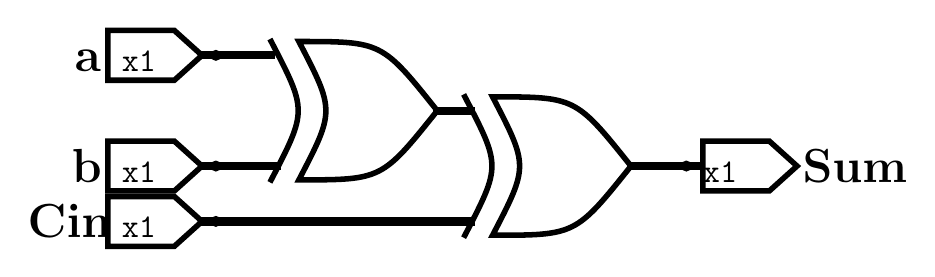
\begin{tikzpicture}[x=1pt,y=-1pt,line cap=rect]
\def\logisimfontA#1{\fontfamily{cmr}{#1}} % Replaced by logisim, original font was "SansSerif"
\def\logisimfontB#1{\fontfamily{cmtt}{#1}} % Replaced by logisim, original font was "Monospaced"
\definecolor{custcol_0_0_0}{RGB}{0, 0, 0}
\definecolor{custcol_ff_ff_ff}{RGB}{255, 255, 255}
\draw [line width=3.0pt, custcol_0_0_0 ]  (223.0,55.0) -- (243.0,55.0) ;
\draw [line width=2.0pt, custcol_0_0_0 ]  (153.0,35.0) .. controls  (133.0,10.0)  ..  (103.0,10.0) .. controls  (116.0,35.0)  ..  (103.0,60.0) .. controls  (133.0,60.0)  ..  (153.0,35.0) -- cycle ;
\draw [line width=2.0pt, custcol_0_0_0 ]  (93.0,10.0) .. controls  (106.0,35.0)  ..  (93.0,60.0) ;
\draw [line width=3.0pt, custcol_0_0_0 ]  (68.0,55.0) -- (73.0,55.0) -- (93.0,55.0) -- (95.0,55.0) ;
\draw [line width=2.0pt, custcol_0_0_0 ]  (58.0,64.0) -- (68.0,55.0) -- (58.0,46.0) -- (34.0,46.0) -- (34.0,64.0) -- cycle;
\logisimfontB{\fontsize{12pt}{12pt}\selectfont\node[inner sep=0, outer sep=0, custcol_0_0_0, anchor=base west] at  (39.0,61.0)  {x1};}
\logisimfontA{\fontsize{16pt}{16pt}\fontseries{bx}\selectfont\node[inner sep=0, outer sep=0, custcol_0_0_0, anchor=base west] at  (21.0,61.0)  {b};}
\fill [line width=2.0pt, custcol_0_0_0]  (73.0,55.0) ellipse (2.0 and 2.0 );
\draw [line width=3.0pt, custcol_0_0_0 ]  (68.0,15.0) -- (73.0,15.0) -- (93.0,15.0) -- (93.0,15.0) ;
\draw [line width=2.0pt, custcol_0_0_0 ]  (58.0,24.0) -- (68.0,15.0) -- (58.0,6.0) -- (34.0,6.0) -- (34.0,24.0) -- cycle;
\logisimfontB{\fontsize{12pt}{12pt}\selectfont\node[inner sep=0, outer sep=0, custcol_0_0_0, anchor=base west] at  (39.0,21.0)  {x1};}
\logisimfontA{\fontsize{16pt}{16pt}\fontseries{bx}\selectfont\node[inner sep=0, outer sep=0, custcol_0_0_0, anchor=base west] at  (22.0,21.0)  {a};}
\fill [line width=2.0pt, custcol_0_0_0]  (73.0,15.0) ellipse (2.0 and 2.0 );
\draw [line width=2.0pt, custcol_0_0_0 ]  (58.0,84.0) -- (68.0,75.0) -- (58.0,66.0) -- (34.0,66.0) -- (34.0,84.0) -- cycle;
\logisimfontB{\fontsize{12pt}{12pt}\selectfont\node[inner sep=0, outer sep=0, custcol_0_0_0, anchor=base west] at  (39.0,81.0)  {x1};}
\logisimfontA{\fontsize{16pt}{16pt}\fontseries{bx}\selectfont\node[inner sep=0, outer sep=0, custcol_0_0_0, anchor=base west] at  (5.0,81.0)  {Cin};}
\fill [line width=2.0pt, custcol_0_0_0]  (73.0,75.0) ellipse (2.0 and 2.0 );
\draw [line width=3.0pt, custcol_0_0_0 ]  (153.0,35.0) -- (163.0,35.0) -- (165.0,35.0) ;
\draw [line width=3.0pt, custcol_0_0_0 ]  (68.0,75.0) -- (73.0,75.0) -- (163.0,75.0) -- (165.0,75.0) ;
\draw [line width=2.0pt, custcol_0_0_0 ]  (223.0,55.0) .. controls  (203.0,30.0)  ..  (173.0,30.0) .. controls  (186.0,55.0)  ..  (173.0,80.0) .. controls  (203.0,80.0)  ..  (223.0,55.0) -- cycle ;
\draw [line width=2.0pt, custcol_0_0_0 ]  (163.0,30.0) .. controls  (176.0,55.0)  ..  (163.0,80.0) ;
\draw [line width=3.0pt, custcol_0_0_0 ]  (247.0,55.0) -- (244.0,55.0) ;
\draw [line width=2.0pt, custcol_0_0_0 ]  (273.0,46.0) -- (283.0,55.0) -- (273.0,64.0) -- (249.0,64.0) -- (249.0,46.0) -- cycle;
\logisimfontB{\fontsize{12pt}{12pt}\selectfont\node[inner sep=0, outer sep=0, custcol_0_0_0, anchor=base west] at  (249.0,61.0)  {x1};}
\logisimfontA{\fontsize{16pt}{16pt}\fontseries{bx}\selectfont\node[inner sep=0, outer sep=0, custcol_0_0_0, anchor=base west] at  (285.0,61.0)  {Sum};}
\fill [line width=2.0pt, custcol_0_0_0]  (243.0,55.0) ellipse (2.0 and 2.0 );
\end{tikzpicture}
}

				\label{fig:somadorcompletoparte01}
			\end{figure}
	\end{columns}
\end{frame}
\begin{frame}
	\frametitle{Somador completo}
	\par Um somador completo deve não apenas receber um $C_{in}$ como também gerar um $C_{out}$. Portanto, é necessário determinar como o $C_{out}$ é obtido.
	\begin{table}[h!]
		\centering
		\begin{tabular}{|c|c|c|c|}
			\hline
			a & b & $C_{in}$ & $C_{out}$ \\
			\hline
			0 & 0 & 0 & \pause 0 \\
			0 & 0 & 1 & \pause 0 \\
			0 & 1 & 0 & \pause 0 \\
			0 & 1 & 1 & \pause 1 \\
			1 & 0 & 0 & \pause 0 \\
			1 & 0 & 1 & \pause 1 \\
			1 & 1 & 0 & \pause 1 \\
			1 & 1 & 1 & \pause 1 \\
			\hline
		\end{tabular}
		\caption{Tabela verdade de $C_{out}$ para somador completo}
		\label{tab:carry_out}
	\end{table}
\end{frame}

\begin{frame}
	\frametitle{Somador completo}
	\framesubtitle{\textbf{Prática dirigida}}
	\par A partir da tabela-verdade mostrada determine a expressão algébrica booleana correspondente e o respectivo circuito de $C_{out}$\footnote[frame]{boa sorte...}.
	
	\begin{columns}
		\column{.6\linewidth}
			\begin{table}[h!]
				\centering
				\begin{tabular}{|c|c|c|c|}
					\hline
					a & b & $C_{in}$ & $C_{out}$ \\
					\hline
					0 & 0 & 0 & 0 \\
					0 & 0 & 1 & 0 \\
					0 & 1 & 0 & 0 \\
					0 & 1 & 1 & 1 \\
					1 & 0 & 0 & 0 \\
					1 & 0 & 1 & 1 \\
					1 & 1 & 0 & 1 \\
					1 & 1 & 1 & 1 \\
					\hline
				\end{tabular}
				\caption{Tabela-verdade de $C_{out}$ para somador completo}
				\label{tab:carry_out2}
			\end{table}
		\column{.4\linewidth}
			\par Para facilitar a notação considerando $c=C_{in}$ temos por \textit{mimtermos}:
			\begin{equation}
				\begin{aligned}
					&(\overline{a}bc)+(a\overline{b}c)+(ab\overline{c})+(abc) = \\
				\end{aligned}
			\end{equation}
	\end{columns}
\end{frame}

\begin{frame}
	\frametitle{Somador completo}
	\framesubtitle{\textbf{Prática dirigida}}
	\begin{columns}
		\column{.5\linewidth}
			\begin{equation}
				\begin{aligned}
					&(\overline{a}bc)+(a\overline{b}c)+(ab\overline{c})+(abc) = \\ \pause
					&\text{reorganizando:} \\
					&(a\overline{b}c)+(ab\overline{c})+(abc)+(\overline{a}bc) = \\ \pause
					&\text{pondo \textbf{a} em evidência:} \\
					&a.(\overline{b}c+b\overline{c}+bc)+(\overline{a}bc) = \\ \pause
					&\text{pondo \textbf{c} em evidência} \\
					&a.(c.(\overline{b}+b)+b\overline{c})+(\overline{a}bc) = \\ \pause
					&a.(c.1+b\overline{c})+(\overline{a}bc) = \\ \pause
					&a.(c+b\overline{c})+(\overline{a}bc) = \\ \pause
				\end{aligned}
			\end{equation}
		\column{.5\linewidth}
			\begin{equation}
				\begin{aligned}
					&\text{usando o teorema:} x+\overline{x}y = x+y \\ \pause
					&a.(c+b)+(\overline{a}bc) = \\
					&ac+ab+\overline{a}bc = \\ 
					&\text{colocando \textbf{b} em evidência:} \\ \pause
					&ac+b.(a+\overline{a}c) = \\
					&\text{usando o teorema:} x+\overline{x}y = x+y \\ \pause
					&ac+b.(a+c) = \\
					&\boxed{ac+ba+bc}
				\end{aligned}
			\end{equation}
	\end{columns}
\end{frame}

\begin{frame}
	\frametitle{Somador completo}
	\framesubtitle{\textbf{Prática dirigida}}
	\par Portanto o circuito do $C_{out}$ fica assim:
	\begin{figure}
		\centering
		% Important: If latex complains about unicode characters,
% please use "\usepackage[utf8x]{inputenc}" in your preamble
% You can change the size of the picture by putting it into the construct:
% 1) \resizebox{10cm}{!}{"below picture"} to scale horizontally to 10 cm
% 2) \resizebox{!}{15cm}{"below picture"} to scale vertically to 15 cm
% 3) \resizebox{10cm}{15cm}{"below picture"} a combination of above two
% It is not recomended to use the scale option of the tikzpicture environment.
\resizebox{10cm}{!}{
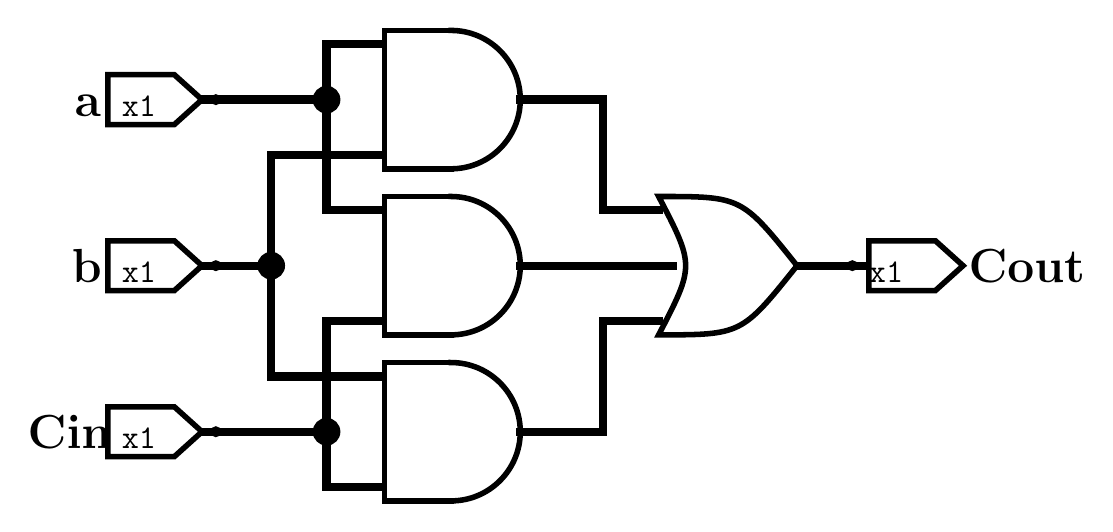
\begin{tikzpicture}[x=1pt,y=-1pt,line cap=rect]
\def\logisimfontA#1{\fontfamily{cmr}{#1}} % Replaced by logisim, original font was "SansSerif"
\def\logisimfontB#1{\fontfamily{cmtt}{#1}} % Replaced by logisim, original font was "Monospaced"
\definecolor{custcol_0_0_0}{RGB}{0, 0, 0}
\definecolor{custcol_ff_ff_ff}{RGB}{255, 255, 255}
\draw [line width=3.0pt, custcol_0_0_0 ]  (283.0,90.0) -- (303.0,90.0) ;
\draw [line width=3.0pt, custcol_0_0_0 ]  (133.0,50.0) -- (93.0,50.0) -- (93.0,90.0) ;
\draw [line width=3.0pt, custcol_0_0_0 ]  (113.0,30.0) -- (113.0,70.0) -- (133.0,70.0) ;
\draw [line width=3.0pt, custcol_0_0_0 ]  (133.0,110.0) -- (113.0,110.0) -- (113.0,150.0) ;
\fill [line width=3.0pt, custcol_0_0_0]  (93.0,90.0) ellipse (5.0 and 5.0 );
\fill [line width=3.0pt, custcol_0_0_0]  (113.0,150.0) ellipse (5.0 and 5.0 );
\fill [line width=3.0pt, custcol_0_0_0]  (113.0,30.0) ellipse (5.0 and 5.0 );
\draw [line width=2.0pt, custcol_0_0_0] (158.0,175.0) arc (90.0:-90.0:25.0 and 25.0 );
\draw [line width=2.0pt, custcol_0_0_0 ]  (158.0,125.0) -- (134.0,125.0) -- (134.0,175.0) -- (158.0,175.0) ;
\draw [line width=2.0pt, custcol_0_0_0] (158.0,115.0) arc (90.0:-90.0:25.0 and 25.0 );
\draw [line width=2.0pt, custcol_0_0_0 ]  (158.0,65.0) -- (134.0,65.0) -- (134.0,115.0) -- (158.0,115.0) ;
\draw [line width=2.0pt, custcol_0_0_0] (158.0,55.0) arc (90.0:-90.0:25.0 and 25.0 );
\draw [line width=2.0pt, custcol_0_0_0 ]  (158.0,5.0) -- (134.0,5.0) -- (134.0,55.0) -- (158.0,55.0) ;
\draw [line width=3.0pt, custcol_0_0_0 ]  (68.0,90.0) -- (73.0,90.0) -- (93.0,90.0) -- (93.0,130.0) -- (133.0,130.0) ;
\draw [line width=2.0pt, custcol_0_0_0 ]  (58.0,99.0) -- (68.0,90.0) -- (58.0,81.0) -- (34.0,81.0) -- (34.0,99.0) -- cycle;
\logisimfontB{\fontsize{12pt}{12pt}\selectfont\node[inner sep=0, outer sep=0, custcol_0_0_0, anchor=base west] at  (39.0,96.0)  {x1};}
\logisimfontA{\fontsize{16pt}{16pt}\fontseries{bx}\selectfont\node[inner sep=0, outer sep=0, custcol_0_0_0, anchor=base west] at  (21.0,96.0)  {b};}
\fill [line width=2.0pt, custcol_0_0_0]  (73.0,90.0) ellipse (2.0 and 2.0 );
\draw [line width=3.0pt, custcol_0_0_0 ]  (68.0,30.0) -- (73.0,30.0) -- (113.0,30.0) -- (113.0,10.0) -- (133.0,10.0) ;
\draw [line width=2.0pt, custcol_0_0_0 ]  (58.0,39.0) -- (68.0,30.0) -- (58.0,21.0) -- (34.0,21.0) -- (34.0,39.0) -- cycle;
\logisimfontB{\fontsize{12pt}{12pt}\selectfont\node[inner sep=0, outer sep=0, custcol_0_0_0, anchor=base west] at  (39.0,36.0)  {x1};}
\logisimfontA{\fontsize{16pt}{16pt}\fontseries{bx}\selectfont\node[inner sep=0, outer sep=0, custcol_0_0_0, anchor=base west] at  (22.0,36.0)  {a};}
\fill [line width=2.0pt, custcol_0_0_0]  (73.0,30.0) ellipse (2.0 and 2.0 );
\draw [line width=3.0pt, custcol_0_0_0 ]  (68.0,150.0) -- (73.0,150.0) -- (113.0,150.0) -- (113.0,170.0) -- (133.0,170.0) ;
\draw [line width=2.0pt, custcol_0_0_0 ]  (58.0,159.0) -- (68.0,150.0) -- (58.0,141.0) -- (34.0,141.0) -- (34.0,159.0) -- cycle;
\logisimfontB{\fontsize{12pt}{12pt}\selectfont\node[inner sep=0, outer sep=0, custcol_0_0_0, anchor=base west] at  (39.0,156.0)  {x1};}
\logisimfontA{\fontsize{16pt}{16pt}\fontseries{bx}\selectfont\node[inner sep=0, outer sep=0, custcol_0_0_0, anchor=base west] at  (5.0,156.0)  {Cin};}
\fill [line width=2.0pt, custcol_0_0_0]  (73.0,150.0) ellipse (2.0 and 2.0 );
\draw [line width=3.0pt, custcol_0_0_0 ]  (183.0,30.0) -- (213.0,30.0) -- (213.0,70.0) -- (233.0,70.0) -- (233.0,70.0) ;
\draw [line width=3.0pt, custcol_0_0_0 ]  (183.0,90.0) -- (233.0,90.0) -- (238.0,90.0) ;
\draw [line width=3.0pt, custcol_0_0_0 ]  (233.0,110.0) -- (233.0,110.0) -- (213.0,110.0) -- (213.0,150.0) -- (183.0,150.0) ;
\draw [line width=2.0pt, custcol_0_0_0 ]  (283.0,90.0) .. controls  (263.0,65.0)  ..  (233.0,65.0) .. controls  (246.0,90.0)  ..  (233.0,115.0) .. controls  (263.0,115.0)  ..  (283.0,90.0) -- cycle ;
\draw [line width=3.0pt, custcol_0_0_0 ]  (307.0,90.0) -- (304.0,90.0) ;
\draw [line width=2.0pt, custcol_0_0_0 ]  (333.0,81.0) -- (343.0,90.0) -- (333.0,99.0) -- (309.0,99.0) -- (309.0,81.0) -- cycle;
\logisimfontB{\fontsize{12pt}{12pt}\selectfont\node[inner sep=0, outer sep=0, custcol_0_0_0, anchor=base west] at  (309.0,96.0)  {x1};}
\logisimfontA{\fontsize{16pt}{16pt}\fontseries{bx}\selectfont\node[inner sep=0, outer sep=0, custcol_0_0_0, anchor=base west] at  (345.0,96.0)  {Cout};}
\fill [line width=2.0pt, custcol_0_0_0]  (303.0,90.0) ellipse (2.0 and 2.0 );
\end{tikzpicture}
}

		\label{fig:somadorcompletoparte02}
	\end{figure}
\end{frame}

\begin{frame}
	\frametitle{Somador completo}
	\framesubtitle{\textbf{Prática dirigida}}
	\par Portanto o circuito \textbf{somador completo} ou \textbf{Full adder} fica assim:
	\begin{figure}
		\centering
		% Important: If latex complains about unicode characters,
% please use "\usepackage[utf8x]{inputenc}" in your preamble
% You can change the size of the picture by putting it into the construct:
% 1) \resizebox{10cm}{!}{"below picture"} to scale horizontally to 10 cm
% 2) \resizebox{!}{15cm}{"below picture"} to scale vertically to 15 cm
% 3) \resizebox{10cm}{15cm}{"below picture"} a combination of above two
% It is not recomended to use the scale option of the tikzpicture environment.
\resizebox{7cm}{!}{
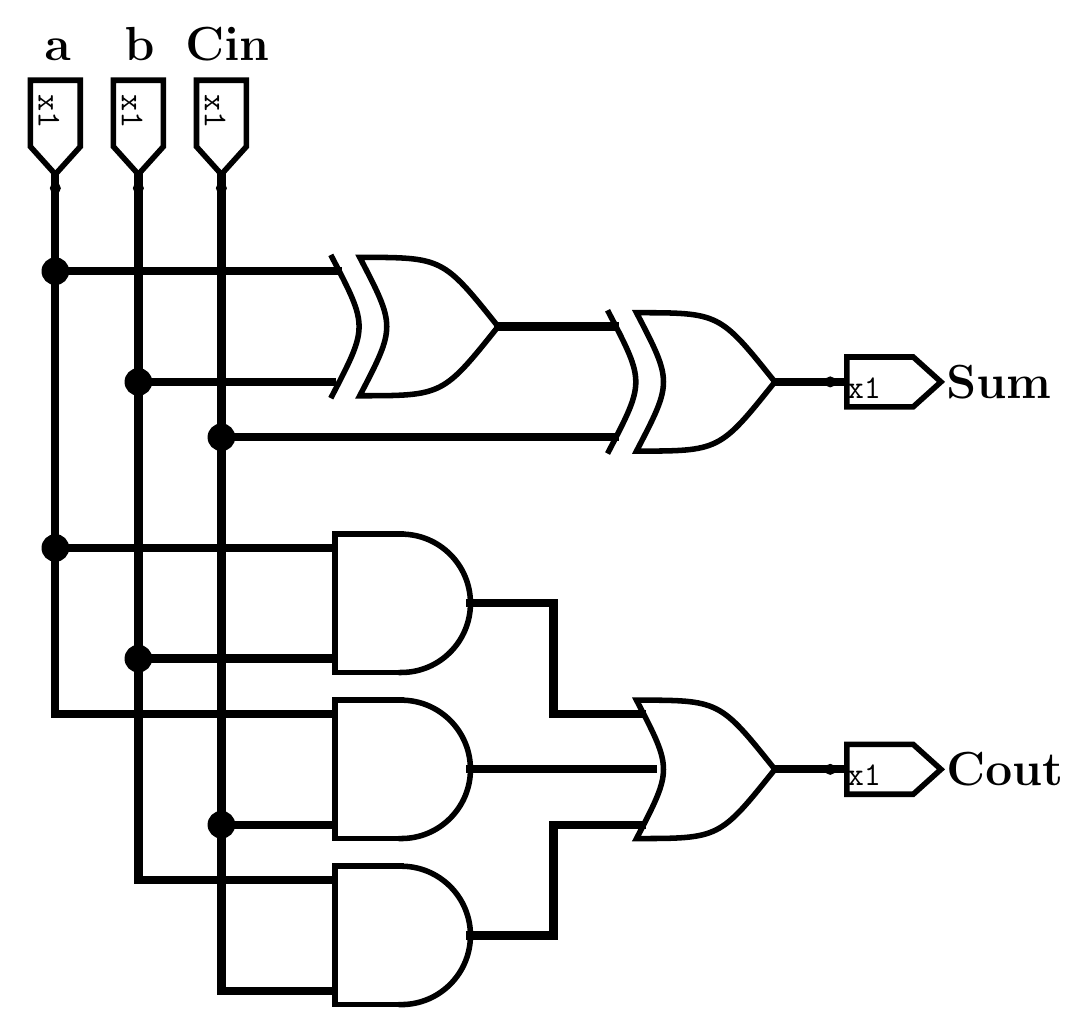
\begin{tikzpicture}[x=1pt,y=-1pt,line cap=rect]
\def\logisimfontA#1{\fontfamily{cmr}{#1}} % Replaced by logisim, original font was "SansSerif"
\def\logisimfontB#1{\fontfamily{cmtt}{#1}} % Replaced by logisim, original font was "Monospaced"
\definecolor{custcol_0_0_0}{RGB}{0, 0, 0}
\definecolor{custcol_ff_ff_ff}{RGB}{255, 255, 255}
\draw [line width=3.0pt, custcol_0_0_0 ]  (15.0,94.0) -- (15.0,194.0) -- (115.0,194.0) ;
\draw [line width=3.0pt, custcol_0_0_0 ]  (275.0,134.0) -- (295.0,134.0) ;
\draw [line width=3.0pt, custcol_0_0_0 ]  (275.0,274.0) -- (295.0,274.0) ;
\draw [line width=3.0pt, custcol_0_0_0 ]  (15.0,194.0) -- (15.0,254.0) -- (115.0,254.0) ;
\draw [line width=3.0pt, custcol_0_0_0 ]  (75.0,294.0) -- (75.0,354.0) -- (115.0,354.0) ;
\draw [line width=3.0pt, custcol_0_0_0 ]  (45.0,234.0) -- (115.0,234.0) ;
\fill [line width=3.0pt, custcol_0_0_0]  (45.0,134.0) ellipse (5.0 and 5.0 );
\fill [line width=3.0pt, custcol_0_0_0]  (15.0,194.0) ellipse (5.0 and 5.0 );
\fill [line width=3.0pt, custcol_0_0_0]  (75.0,154.0) ellipse (5.0 and 5.0 );
\fill [line width=3.0pt, custcol_0_0_0]  (15.0,94.0) ellipse (5.0 and 5.0 );
\fill [line width=3.0pt, custcol_0_0_0]  (75.0,294.0) ellipse (5.0 and 5.0 );
\fill [line width=3.0pt, custcol_0_0_0]  (45.0,234.0) ellipse (5.0 and 5.0 );
\draw [line width=3.0pt, custcol_0_0_0 ]  (75.0,59.0) -- (75.0,64.0) -- (75.0,154.0) -- (75.0,294.0) -- (115.0,294.0) ;
\draw [line width=2.0pt, custcol_0_0_0 ]  (66.0,49.0) -- (75.0,59.0) -- (84.0,49.0) -- (84.0,25.0) -- (66.0,25.0) -- cycle;
\logisimfontB{\fontsize{12pt}{12pt}\selectfont\node[inner sep=0, outer sep=0, custcol_0_0_0, anchor=base west, rotate=-90.0] at  (69.0,30.0)  {x1};}
\logisimfontA{\fontsize{16pt}{16pt}\fontseries{bx}\selectfont\node[inner sep=0, outer sep=0, custcol_0_0_0, anchor=base west] at  (62.0,18.0)  {Cin};}
\fill [line width=2.0pt, custcol_0_0_0]  (75.0,64.0) ellipse (2.0 and 2.0 );
\draw [line width=2.0pt, custcol_0_0_0 ]  (6.0,49.0) -- (15.0,59.0) -- (24.0,49.0) -- (24.0,25.0) -- (6.0,25.0) -- cycle;
\logisimfontB{\fontsize{12pt}{12pt}\selectfont\node[inner sep=0, outer sep=0, custcol_0_0_0, anchor=base west, rotate=-90.0] at  (9.0,30.0)  {x1};}
\logisimfontA{\fontsize{16pt}{16pt}\fontseries{bx}\selectfont\node[inner sep=0, outer sep=0, custcol_0_0_0, anchor=base west] at  (11.0,18.0)  {a};}
\fill [line width=2.0pt, custcol_0_0_0]  (15.0,64.0) ellipse (2.0 and 2.0 );
\draw [line width=2.0pt, custcol_0_0_0] (140.0,359.0) arc (90.0:-90.0:25.0 and 25.0 );
\draw [line width=2.0pt, custcol_0_0_0 ]  (140.0,309.0) -- (116.0,309.0) -- (116.0,359.0) -- (140.0,359.0) ;
\draw [line width=3.0pt, custcol_0_0_0 ]  (165.0,214.0) -- (195.0,214.0) -- (195.0,254.0) -- (225.0,254.0) -- (227.0,254.0) ;
\draw [line width=3.0pt, custcol_0_0_0 ]  (165.0,274.0) -- (225.0,274.0) -- (231.0,274.0) ;
\draw [line width=3.0pt, custcol_0_0_0 ]  (165.0,334.0) -- (195.0,334.0) -- (195.0,294.0) -- (225.0,294.0) -- (227.0,294.0) ;
\draw [line width=2.0pt, custcol_0_0_0 ]  (275.0,274.0) .. controls  (255.0,249.0)  ..  (225.0,249.0) .. controls  (238.0,274.0)  ..  (225.0,299.0) .. controls  (255.0,299.0)  ..  (275.0,274.0) -- cycle ;
\draw [line width=3.0pt, custcol_0_0_0 ]  (175.0,114.0) -- (215.0,114.0) -- (217.0,114.0) ;
\draw [line width=3.0pt, custcol_0_0_0 ]  (75.0,154.0) -- (215.0,154.0) -- (217.0,154.0) ;
\draw [line width=2.0pt, custcol_0_0_0 ]  (275.0,134.0) .. controls  (255.0,109.0)  ..  (225.0,109.0) .. controls  (238.0,134.0)  ..  (225.0,159.0) .. controls  (255.0,159.0)  ..  (275.0,134.0) -- cycle ;
\draw [line width=2.0pt, custcol_0_0_0 ]  (215.0,109.0) .. controls  (228.0,134.0)  ..  (215.0,159.0) ;
\draw [line width=3.0pt, custcol_0_0_0 ]  (299.0,134.0) -- (296.0,134.0) ;
\draw [line width=2.0pt, custcol_0_0_0 ]  (325.0,125.0) -- (335.0,134.0) -- (325.0,143.0) -- (301.0,143.0) -- (301.0,125.0) -- cycle;
\logisimfontB{\fontsize{12pt}{12pt}\selectfont\node[inner sep=0, outer sep=0, custcol_0_0_0, anchor=base west] at  (301.0,140.0)  {x1};}
\logisimfontA{\fontsize{16pt}{16pt}\fontseries{bx}\selectfont\node[inner sep=0, outer sep=0, custcol_0_0_0, anchor=base west] at  (337.0,140.0)  {Sum};}
\fill [line width=2.0pt, custcol_0_0_0]  (295.0,134.0) ellipse (2.0 and 2.0 );
\draw [line width=3.0pt, custcol_0_0_0 ]  (45.0,59.0) -- (45.0,64.0) -- (45.0,134.0) -- (45.0,234.0) -- (45.0,314.0) -- (115.0,314.0) ;
\draw [line width=2.0pt, custcol_0_0_0 ]  (36.0,49.0) -- (45.0,59.0) -- (54.0,49.0) -- (54.0,25.0) -- (36.0,25.0) -- cycle;
\logisimfontB{\fontsize{12pt}{12pt}\selectfont\node[inner sep=0, outer sep=0, custcol_0_0_0, anchor=base west, rotate=-90.0] at  (39.0,30.0)  {x1};}
\logisimfontA{\fontsize{16pt}{16pt}\fontseries{bx}\selectfont\node[inner sep=0, outer sep=0, custcol_0_0_0, anchor=base west] at  (40.0,18.0)  {b};}
\fill [line width=2.0pt, custcol_0_0_0]  (45.0,64.0) ellipse (2.0 and 2.0 );
\draw [line width=2.0pt, custcol_0_0_0] (140.0,299.0) arc (90.0:-90.0:25.0 and 25.0 );
\draw [line width=2.0pt, custcol_0_0_0 ]  (140.0,249.0) -- (116.0,249.0) -- (116.0,299.0) -- (140.0,299.0) ;
\draw [line width=3.0pt, custcol_0_0_0 ]  (299.0,274.0) -- (296.0,274.0) ;
\draw [line width=2.0pt, custcol_0_0_0 ]  (325.0,265.0) -- (335.0,274.0) -- (325.0,283.0) -- (301.0,283.0) -- (301.0,265.0) -- cycle;
\logisimfontB{\fontsize{12pt}{12pt}\selectfont\node[inner sep=0, outer sep=0, custcol_0_0_0, anchor=base west] at  (301.0,280.0)  {x1};}
\logisimfontA{\fontsize{16pt}{16pt}\fontseries{bx}\selectfont\node[inner sep=0, outer sep=0, custcol_0_0_0, anchor=base west] at  (337.0,280.0)  {Cout};}
\fill [line width=2.0pt, custcol_0_0_0]  (295.0,274.0) ellipse (2.0 and 2.0 );
\draw [line width=2.0pt, custcol_0_0_0] (140.0,239.0) arc (90.0:-90.0:25.0 and 25.0 );
\draw [line width=2.0pt, custcol_0_0_0 ]  (140.0,189.0) -- (116.0,189.0) -- (116.0,239.0) -- (140.0,239.0) ;
\draw [line width=3.0pt, custcol_0_0_0 ]  (15.0,59.0) -- (15.0,64.0) -- (15.0,94.0) -- (115.0,94.0) -- (117.0,94.0) ;
\draw [line width=3.0pt, custcol_0_0_0 ]  (45.0,134.0) -- (115.0,134.0) -- (115.0,134.0) ;
\draw [line width=2.0pt, custcol_0_0_0 ]  (175.0,114.0) .. controls  (155.0,89.0)  ..  (125.0,89.0) .. controls  (138.0,114.0)  ..  (125.0,139.0) .. controls  (155.0,139.0)  ..  (175.0,114.0) -- cycle ;
\draw [line width=2.0pt, custcol_0_0_0 ]  (115.0,89.0) .. controls  (128.0,114.0)  ..  (115.0,139.0) ;
\end{tikzpicture}
}

		\label{fig:somadorcompleto}
	\end{figure}
\end{frame}

\begin{frame}
	\frametitle{Somador completo - Gambiarra}
	\par Usando somadores incompletos podemos fazer um completo:
	\begin{figure}
		\centering
		% Important: If latex complains about unicode characters,
% please use "\usepackage[utf8x]{inputenc}" in your preamble
% You can change the size of the picture by putting it into the construct:
% 1) \resizebox{10cm}{!}{"below picture"} to scale horizontally to 10 cm
% 2) \resizebox{!}{15cm}{"below picture"} to scale vertically to 15 cm
% 3) \resizebox{10cm}{15cm}{"below picture"} a combination of above two
% It is not recomended to use the scale option of the tikzpicture environment.
\resizebox{15cm}{!}{
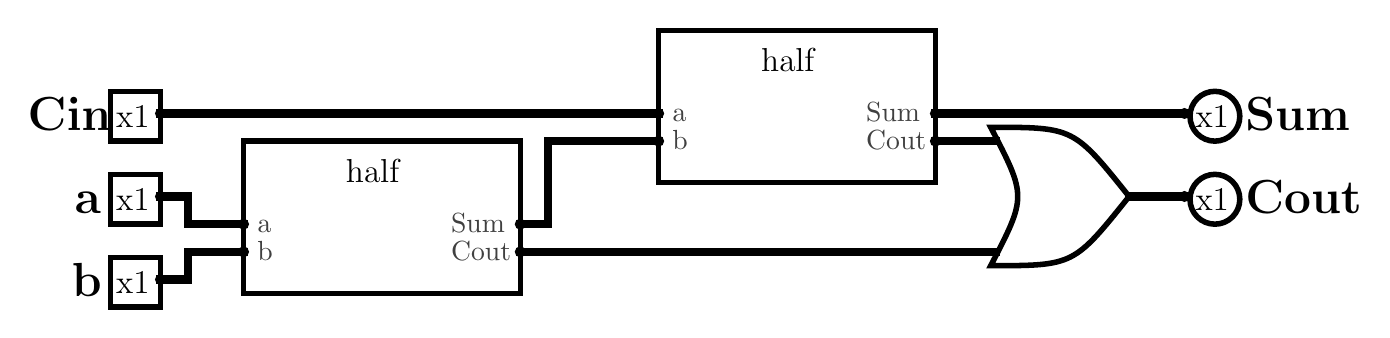
\begin{tikzpicture}[x=1pt,y=-1pt,line cap=rect]
\def\logisimfontA#1{\fontfamily{cmr}{#1}} % Replaced by logisim, original font was "SansSerif"
\definecolor{custcol_0_0_0}{RGB}{0, 0, 0}
\definecolor{custcol_40_40_40}{RGB}{64, 64, 64}
\definecolor{custcol_ff_ff_ff}{RGB}{255, 255, 255}
\draw [line width=3.0pt, custcol_0_0_0 ]  (333.0,36.0) -- (423.0,36.0) ;
\draw [line width=3.0pt, custcol_0_0_0 ]  (403.0,66.0) -- (423.0,66.0) ;
\draw [line width=3.0pt, custcol_0_0_0 ]  (53.0,36.0) -- (233.0,36.0) ;
\draw [line width=3.0pt, custcol_0_0_0 ]  (53.0,66.0) -- (63.0,66.0) -- (63.0,76.0) -- (83.0,76.0) ;
\draw [line width=3.0pt, custcol_0_0_0 ]  (53.0,96.0) -- (63.0,96.0) -- (63.0,86.0) -- (83.0,86.0) ;
\draw [line width=3.0pt, custcol_0_0_0 ]  (183.0,76.0) -- (193.0,76.0) -- (193.0,46.0) -- (233.0,46.0) ;
\draw [line width=2.0pt, custcol_0_0_0 ]  (233.0,6.0) -- (332.0,6.0) ;
\draw [line width=2.0pt, custcol_0_0_0 ]  (333.0,6.0) -- (333.0,60.0) ;
\draw [line width=2.0pt, custcol_0_0_0 ]  (333.0,61.0) -- (234.0,61.0) ;
\draw [line width=2.0pt, custcol_0_0_0 ]  (233.0,61.0) -- (233.0,7.0) ;
\logisimfontA{\fontsize{10pt}{10pt}\selectfont\node[inner sep=0, outer sep=0, custcol_40_40_40, anchor=base west] at  (238.0,39.0)  {a};}
\logisimfontA{\fontsize{10pt}{10pt}\selectfont\node[inner sep=0, outer sep=0, custcol_40_40_40, anchor=base west] at  (238.0,49.0)  {b};}
\logisimfontA{\fontsize{10pt}{10pt}\selectfont\node[inner sep=0, outer sep=0, custcol_40_40_40, anchor=base west] at  (308.0,39.0)  {Sum};}
\logisimfontA{\fontsize{10pt}{10pt}\selectfont\node[inner sep=0, outer sep=0, custcol_40_40_40, anchor=base west] at  (308.0,49.0)  {Cout};}
\logisimfontA{\fontsize{12pt}{12pt}\selectfont\node[inner sep=0, outer sep=0, custcol_0_0_0, anchor=base west] at  (270.0,21.0)  {half};}
\fill [line width=1.0pt, custcol_0_0_0]  (233.0,36.0) ellipse (2.0 and 2.0 );
\fill [line width=1.0pt, custcol_0_0_0]  (233.0,46.0) ellipse (2.0 and 2.0 );
\fill [line width=1.0pt, custcol_0_0_0]  (333.0,36.0) ellipse (2.0 and 2.0 );
\fill [line width=1.0pt, custcol_0_0_0]  (333.0,46.0) ellipse (2.0 and 2.0 );
\draw [line width=2.0pt, custcol_0_0_0 ]  (83.0,46.0) -- (182.0,46.0) ;
\draw [line width=2.0pt, custcol_0_0_0 ]  (183.0,46.0) -- (183.0,100.0) ;
\draw [line width=2.0pt, custcol_0_0_0 ]  (183.0,101.0) -- (84.0,101.0) ;
\draw [line width=2.0pt, custcol_0_0_0 ]  (83.0,101.0) -- (83.0,47.0) ;
\logisimfontA{\fontsize{10pt}{10pt}\selectfont\node[inner sep=0, outer sep=0, custcol_40_40_40, anchor=base west] at  (88.0,79.0)  {a};}
\logisimfontA{\fontsize{10pt}{10pt}\selectfont\node[inner sep=0, outer sep=0, custcol_40_40_40, anchor=base west] at  (88.0,89.0)  {b};}
\logisimfontA{\fontsize{10pt}{10pt}\selectfont\node[inner sep=0, outer sep=0, custcol_40_40_40, anchor=base west] at  (158.0,79.0)  {Sum};}
\logisimfontA{\fontsize{10pt}{10pt}\selectfont\node[inner sep=0, outer sep=0, custcol_40_40_40, anchor=base west] at  (158.0,89.0)  {Cout};}
\logisimfontA{\fontsize{12pt}{12pt}\selectfont\node[inner sep=0, outer sep=0, custcol_0_0_0, anchor=base west] at  (120.0,61.0)  {half};}
\fill [line width=1.0pt, custcol_0_0_0]  (83.0,76.0) ellipse (2.0 and 2.0 );
\fill [line width=1.0pt, custcol_0_0_0]  (83.0,86.0) ellipse (2.0 and 2.0 );
\fill [line width=1.0pt, custcol_0_0_0]  (183.0,76.0) ellipse (2.0 and 2.0 );
\fill [line width=1.0pt, custcol_0_0_0]  (183.0,86.0) ellipse (2.0 and 2.0 );
\draw [line width=2.0pt, custcol_0_0_0 ]  (35.0,28.0) -- (52.0,28.0) ;
\draw [line width=2.0pt, custcol_0_0_0 ]  (53.0,28.0) -- (53.0,45.0) ;
\draw [line width=2.0pt, custcol_0_0_0 ]  (53.0,46.0) -- (36.0,46.0) ;
\draw [line width=2.0pt, custcol_0_0_0 ]  (35.0,46.0) -- (35.0,29.0) ;
\logisimfontA{\fontsize{12pt}{12pt}\selectfont\node[inner sep=0, outer sep=0, custcol_0_0_0, anchor=base west] at  (37.0,41.0)  {x1};}
\logisimfontA{\fontsize{16pt}{16pt}\fontseries{bx}\selectfont\node[inner sep=0, outer sep=0, custcol_0_0_0, anchor=base west] at  (5.0,42.0)  {Cin};}
\fill [line width=2.0pt, custcol_0_0_0]  (53.0,36.0) ellipse (2.0 and 2.0 );
\draw [line width=2.0pt, custcol_0_0_0 ]  (35.0,58.0) -- (52.0,58.0) ;
\draw [line width=2.0pt, custcol_0_0_0 ]  (53.0,58.0) -- (53.0,75.0) ;
\draw [line width=2.0pt, custcol_0_0_0 ]  (53.0,76.0) -- (36.0,76.0) ;
\draw [line width=2.0pt, custcol_0_0_0 ]  (35.0,76.0) -- (35.0,59.0) ;
\logisimfontA{\fontsize{12pt}{12pt}\selectfont\node[inner sep=0, outer sep=0, custcol_0_0_0, anchor=base west] at  (37.0,71.0)  {x1};}
\logisimfontA{\fontsize{16pt}{16pt}\fontseries{bx}\selectfont\node[inner sep=0, outer sep=0, custcol_0_0_0, anchor=base west] at  (22.0,72.0)  {a};}
\fill [line width=2.0pt, custcol_0_0_0]  (53.0,66.0) ellipse (2.0 and 2.0 );
\draw [line width=2.0pt, custcol_0_0_0 ]  (35.0,88.0) -- (52.0,88.0) ;
\draw [line width=2.0pt, custcol_0_0_0 ]  (53.0,88.0) -- (53.0,105.0) ;
\draw [line width=2.0pt, custcol_0_0_0 ]  (53.0,106.0) -- (36.0,106.0) ;
\draw [line width=2.0pt, custcol_0_0_0 ]  (35.0,106.0) -- (35.0,89.0) ;
\logisimfontA{\fontsize{12pt}{12pt}\selectfont\node[inner sep=0, outer sep=0, custcol_0_0_0, anchor=base west] at  (37.0,101.0)  {x1};}
\logisimfontA{\fontsize{16pt}{16pt}\fontseries{bx}\selectfont\node[inner sep=0, outer sep=0, custcol_0_0_0, anchor=base west] at  (21.0,102.0)  {b};}
\fill [line width=2.0pt, custcol_0_0_0]  (53.0,96.0) ellipse (2.0 and 2.0 );
\draw [line width=3.0pt, custcol_0_0_0 ]  (333.0,46.0) -- (353.0,46.0) -- (355.0,46.0) ;
\draw [line width=3.0pt, custcol_0_0_0 ]  (183.0,86.0) -- (353.0,86.0) -- (355.0,86.0) ;
\draw [line width=2.0pt, custcol_0_0_0 ]  (403.0,66.0) .. controls  (383.0,41.0)  ..  (353.0,41.0) .. controls  (366.0,66.0)  ..  (353.0,91.0) .. controls  (383.0,91.0)  ..  (403.0,66.0) -- cycle ;
\draw [line width=2.0pt, custcol_0_0_0]  (434.0,67.0) ellipse (9.0 and 9.0 );
\logisimfontA{\fontsize{12pt}{12pt}\selectfont\node[inner sep=0, outer sep=0, custcol_0_0_0, anchor=base west] at  (427.0,71.0)  {x1};}
\logisimfontA{\fontsize{16pt}{16pt}\fontseries{bx}\selectfont\node[inner sep=0, outer sep=0, custcol_0_0_0, anchor=base west] at  (445.0,72.0)  {Cout};}
\fill [line width=2.0pt, custcol_0_0_0]  (423.0,66.0) ellipse (2.0 and 2.0 );
\draw [line width=2.0pt, custcol_0_0_0]  (434.0,37.0) ellipse (9.0 and 9.0 );
\logisimfontA{\fontsize{12pt}{12pt}\selectfont\node[inner sep=0, outer sep=0, custcol_0_0_0, anchor=base west] at  (427.0,41.0)  {x1};}
\logisimfontA{\fontsize{16pt}{16pt}\fontseries{bx}\selectfont\node[inner sep=0, outer sep=0, custcol_0_0_0, anchor=base west] at  (445.0,42.0)  {Sum};}
\fill [line width=2.0pt, custcol_0_0_0]  (423.0,36.0) ellipse (2.0 and 2.0 );
\end{tikzpicture}
}

		\label{fig:somadorcompletogambiarra}
	\end{figure}
\end{frame}

\subsection{Subtratores}

\begin{frame}
	\frametitle{Subtração binária}
	\framesubtitle{Expressão de exemplo}
	\par Abaixo foi realizada uma operação de subtração simples entre dois números binários, a e b, cujo resultado é mostrado na linha marcada com a palavra 'Diff'. '$B_{out}$' significa 'Borrow out', o nosso famoso 'emprestar'. A partir deste exemplo, vamos criar uma tabela-verdade que nos permitirá formular a expressão algébrica booleana e, consequentemente, o circuito subtrator correspondente.
	\begin{table}[h!]
		\centering
		\begin{tabular}{cccc>{\centering\arraybackslash}p{2cm}}
			& 10 & 10 & 10 & $B_{out}$ \\
			1 & 1 & 0 & 0 & $a$\\
			& 1 & 1 & 1 & $b$ \\
			\hline
			& 1 & 0 & 1 & $Diff$ \\
		\end{tabular}
	\end{table}
\end{frame}

\begin{frame}
	\frametitle{Meio subtrator / Subtrator incompleto / Half subtractor}
	\par A tabela-verdade e o circuito mostrados abaixo representam o que chamamos de \textbf{meio subtrator}, \textbf{subtrator incompleto} ou ainda \textit{\textbf{Half subtrator}}. O meio subtrator tem essa denominação porque, apesar de realizar a subtração de dois bits, não considera um bit que possa ter sido emprestado por uma operação de subtração anterior. Dessa forma, o circuito é capaz de trabalhar apenas com a subtração de dois bits, informando se houve necessidade de empréstimo de um bit $B_{out}$. Isso impede a criação de subtratores para números maiores por meio da concatenação de vários circuitos
	\begin{table}[h!]
		\centering
		\begin{tabular}{|c|c|c|c|}
			\hline
			a & b & Diff & \(B_{out}\) \\ \hline
			0 & 0 & 0   & 0          \\ \hline
			0 & 1 & 1   & 1          \\ \hline
			1 & 0 & 1   & 0          \\ \hline
			1 & 1 & 0   & 0          \\ \hline
		\end{tabular}
		\caption{Tabela verdade da diferença binária}
		\label{tab:binary_subtraction}
	\end{table}
\end{frame}

\begin{frame}
	\frametitle{Meio subtrator / Subtrator incompleto / Half subtractor}
	\framesubtitle{\textbf{Prática dirigida} - Tabela verdade da subtração}
	\par Como $Diff$ e $B_{out}$ se comportam? Qual o circuito correspondente?
	\begin{table}[h!]
		\centering
		\begin{tabular}{|c|c|c|c|}
			\hline
			a & b & Diff & \(B_{out}\) \\ \hline
			0 & 0 & 0   & 0          \\ \hline
			0 & 1 & 1   & 1          \\ \hline
			1 & 0 & 1   & 0          \\ \hline
			1 & 1 & 0   & 0          \\ \hline
		\end{tabular}
		\caption{Tabela verdade da diferença binária}
		\label{tab:binary_subtraction2}
	\end{table}
\end{frame}

\begin{frame}
	\frametitle{Meio subtrator / Subtrator incompleto / Half subtractor}
	\framesubtitle{\textbf{Prática dirigida} - Tabela verdade da subtração}
	\begin{columns}
		\column{.5\linewidth}
		\begin{table}[h!]
			\centering
			\begin{tabular}{|c|c|c|c|c|c|}
				\hline
				a & b & Diff & \(B_{out}\)& \(a \oplus b\) & \(\overline{a}.b\) \\ \hline
				0 & 0 & 0   & 0          & 0              & 0             \\ \hline
				0 & 1 & 1   & 1          & 1              & 1             \\ \hline
				1 & 0 & 1   & 0          & 1              & 0             \\ \hline
				1 & 1 & 0   & 0          & 0              & 0             \\ \hline
			\end{tabular}
			\caption{Tabela verdade da diferença binária}
			\label{tab:binary_subtraction3}
		\end{table}
		\pause
		\column{.5\linewidth}
		\begin{figure}
			\centering
			% Important: If latex complains about unicode characters,
% please use "\usepackage[utf8x]{inputenc}" in your preamble
% You can change the size of the picture by putting it into the construct:
% 1) \resizebox{10cm}{!}{"below picture"} to scale horizontally to 10 cm
% 2) \resizebox{!}{15cm}{"below picture"} to scale vertically to 15 cm
% 3) \resizebox{10cm}{15cm}{"below picture"} a combination of above two
% It is not recomended to use the scale option of the tikzpicture environment.
\resizebox{6cm}{!}{
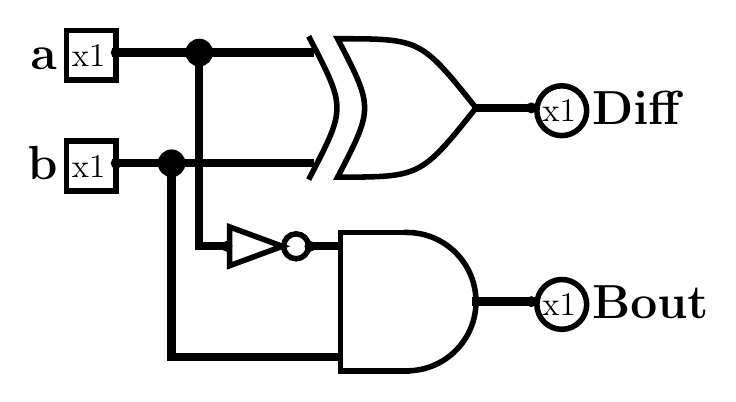
\begin{tikzpicture}[x=1pt,y=-1pt,line cap=rect]
\def\logisimfontA#1{\fontfamily{cmr}{#1}} % Replaced by logisim, original font was "SansSerif"
\definecolor{custcol_0_0_0}{RGB}{0, 0, 0}
\definecolor{custcol_ff_ff_ff}{RGB}{255, 255, 255}
\draw [line width=3.0pt, custcol_0_0_0 ]  (37.0,15.0) -- (67.0,15.0) -- (67.0,85.0) -- (77.0,85.0) ;
\draw [line width=3.0pt, custcol_0_0_0 ]  (107.0,85.0) -- (117.0,85.0) ;
\draw [line width=3.0pt, custcol_0_0_0 ]  (167.0,35.0) -- (187.0,35.0) ;
\draw [line width=3.0pt, custcol_0_0_0 ]  (167.0,105.0) -- (187.0,105.0) ;
\draw [line width=3.0pt, custcol_0_0_0 ]  (37.0,55.0) -- (57.0,55.0) ;
\fill [line width=3.0pt, custcol_0_0_0]  (57.0,55.0) ellipse (5.0 and 5.0 );
\fill [line width=3.0pt, custcol_0_0_0]  (67.0,15.0) ellipse (5.0 and 5.0 );
\draw [line width=2.0pt, custcol_0_0_0 ]  (19.0,7.0) -- (36.0,7.0) ;
\draw [line width=2.0pt, custcol_0_0_0 ]  (37.0,7.0) -- (37.0,24.0) ;
\draw [line width=2.0pt, custcol_0_0_0 ]  (37.0,25.0) -- (20.0,25.0) ;
\draw [line width=2.0pt, custcol_0_0_0 ]  (19.0,25.0) -- (19.0,8.0) ;
\logisimfontA{\fontsize{12pt}{12pt}\selectfont\node[inner sep=0, outer sep=0, custcol_0_0_0, anchor=base west] at  (21.0,20.0)  {x1};}
\logisimfontA{\fontsize{16pt}{16pt}\fontseries{bx}\selectfont\node[inner sep=0, outer sep=0, custcol_0_0_0, anchor=base west] at  (6.0,21.0)  {a};}
\fill [line width=2.0pt, custcol_0_0_0]  (37.0,15.0) ellipse (2.0 and 2.0 );
\draw [line width=2.0pt, custcol_0_0_0 ]  (19.0,47.0) -- (36.0,47.0) ;
\draw [line width=2.0pt, custcol_0_0_0 ]  (37.0,47.0) -- (37.0,64.0) ;
\draw [line width=2.0pt, custcol_0_0_0 ]  (37.0,65.0) -- (20.0,65.0) ;
\draw [line width=2.0pt, custcol_0_0_0 ]  (19.0,65.0) -- (19.0,48.0) ;
\logisimfontA{\fontsize{12pt}{12pt}\selectfont\node[inner sep=0, outer sep=0, custcol_0_0_0, anchor=base west] at  (21.0,60.0)  {x1};}
\logisimfontA{\fontsize{16pt}{16pt}\fontseries{bx}\selectfont\node[inner sep=0, outer sep=0, custcol_0_0_0, anchor=base west] at  (5.0,61.0)  {b};}
\fill [line width=2.0pt, custcol_0_0_0]  (37.0,55.0) ellipse (2.0 and 2.0 );
\draw [line width=3.0pt, custcol_0_0_0 ]  (67.0,15.0) -- (107.0,15.0) -- (107.0,15.0) ;
\draw [line width=3.0pt, custcol_0_0_0 ]  (117.0,125.0) -- (57.0,125.0) -- (57.0,55.0) -- (107.0,55.0) -- (107.0,55.0) ;
\draw [line width=2.0pt, custcol_0_0_0 ]  (167.0,35.0) .. controls  (147.0,10.0)  ..  (117.0,10.0) .. controls  (130.0,35.0)  ..  (117.0,60.0) .. controls  (147.0,60.0)  ..  (167.0,35.0) -- cycle ;
\draw [line width=2.0pt, custcol_0_0_0 ]  (107.0,10.0) .. controls  (120.0,35.0)  ..  (107.0,60.0) ;
\draw [line width=2.0pt, custcol_0_0_0]  (198.0,36.0) ellipse (9.0 and 9.0 );
\logisimfontA{\fontsize{12pt}{12pt}\selectfont\node[inner sep=0, outer sep=0, custcol_0_0_0, anchor=base west] at  (191.0,40.0)  {x1};}
\logisimfontA{\fontsize{16pt}{16pt}\fontseries{bx}\selectfont\node[inner sep=0, outer sep=0, custcol_0_0_0, anchor=base west] at  (209.0,41.0)  {Diff};}
\fill [line width=2.0pt, custcol_0_0_0]  (187.0,35.0) ellipse (2.0 and 2.0 );
\draw [line width=2.0pt, custcol_0_0_0 ]  (97.0,85.0) -- (78.0,78.0) -- (78.0,92.0) -- cycle;
\draw [line width=2.0pt, custcol_0_0_0]  (102.0,85.0) ellipse (4.5 and 4.5 );
\fill [line width=2.0pt, custcol_0_0_0]  (107.0,85.0) ellipse (2.0 and 2.0 );
\fill [line width=2.0pt, custcol_0_0_0]  (77.0,85.0) ellipse (2.0 and 2.0 );
\draw [line width=2.0pt, custcol_0_0_0]  (198.0,106.0) ellipse (9.0 and 9.0 );
\logisimfontA{\fontsize{12pt}{12pt}\selectfont\node[inner sep=0, outer sep=0, custcol_0_0_0, anchor=base west] at  (191.0,110.0)  {x1};}
\logisimfontA{\fontsize{16pt}{16pt}\fontseries{bx}\selectfont\node[inner sep=0, outer sep=0, custcol_0_0_0, anchor=base west] at  (209.0,111.0)  {Bout};}
\fill [line width=2.0pt, custcol_0_0_0]  (187.0,105.0) ellipse (2.0 and 2.0 );
\draw [line width=2.0pt, custcol_0_0_0] (142.0,130.0) arc (90.0:-90.0:25.0 and 25.0 );
\draw [line width=2.0pt, custcol_0_0_0 ]  (142.0,80.0) -- (118.0,80.0) -- (118.0,130.0) -- (142.0,130.0) ;
\end{tikzpicture}
}

			\label{fig:subtratorimcompleto}
		\end{figure}
	\end{columns}
\end{frame}



























\begin{frame}
	\frametitle{Subtrator completo}
	\par Para determinar um subtrator completo, é necessário considerar não apenas as entradas $a$ e $b$, mas também uma entrada $B_{in}$​, que representa o possível bit subtrator vindo do $B_{out}$​ de outro circuito. Dessa forma, o resultado da subtração é alterado, o que, por sua vez, modifica a expressão final e o circuito resultante.
	\par Tenha em mente que $Diff = a-b-B_{in}$.
	\begin{table}[h!]
		\centering
		\begin{tabular}{|c|c|c|c|c|}
			\hline
			a & b & $B_{in}$ & Diff & $B_{out}$ \\
			\hline
			0 & 0 & 0 & 0 & 0 \\
			0 & 0 & 1 & 1 & 1 \\
			0 & 1 & 0 & 1 & 1 \\
			0 & 1 & 1 & 0 & 1 \\
			1 & 0 & 0 & 1 & 0 \\
			1 & 0 & 1 & 0 & 0 \\
			1 & 1 & 0 & 0 & 0 \\
			1 & 1 & 1 & 1 & 1 \\
			\hline
		\end{tabular}
		\caption{Tabela verdade de um subtrator completo}
		\label{tab:full_subtractor}
	\end{table}
\end{frame}

\begin{frame}
	\frametitle{Subtrator completo}
	\framesubtitle{\textbf{Prática guiada}}
	\par Considerando a tabela verdade mostrada determine as expressões algébricas boleanas e os circuitos de $Diff$ e $B_{out}$ correspondentes.
	\begin{columns}
		\column{.5\linewidth}
		\begin{table}[h!]
			\centering
			\begin{tabular}{|c|c|c|c|c|}
				\hline
				a & b & $B_{in}$ & Diff & $B_{out}$ \\
				\hline
				0 & 0 & 0 & 0 & 0 \\
				0 & 0 & 1 & 1 & 1 \\
				0 & 1 & 0 & 1 & 1 \\
				0 & 1 & 1 & 0 & 1 \\
				1 & 0 & 0 & 1 & 0 \\
				1 & 0 & 1 & 0 & 0 \\
				1 & 1 & 0 & 0 & 0 \\
				1 & 1 & 1 & 1 & 1 \\
				\hline
			\end{tabular}
			\caption{Tabela verdade de $B_{in}$ para subtrator completo}
			\label{tab:full_subtractor2}
		\end{table}
		\column{.5\linewidth}
		\pause
		\par Se você olhou bem, economizou tempo! Pois $Diff = a \oplus b \oplus c \therefore$ $\boxed{Diff=a \oplus b \oplus B_{in}}$
		\pause
		\begin{figure}
			\centering
			% Important: If latex complains about unicode characters,
% please use "\usepackage[utf8x]{inputenc}" in your preamble
% You can change the size of the picture by putting it into the construct:
% 1) \resizebox{10cm}{!}{"below picture"} to scale horizontally to 10 cm
% 2) \resizebox{!}{15cm}{"below picture"} to scale vertically to 15 cm
% 3) \resizebox{10cm}{15cm}{"below picture"} a combination of above two
% It is not recomended to use the scale option of the tikzpicture environment.
\resizebox{7cm}{!}{
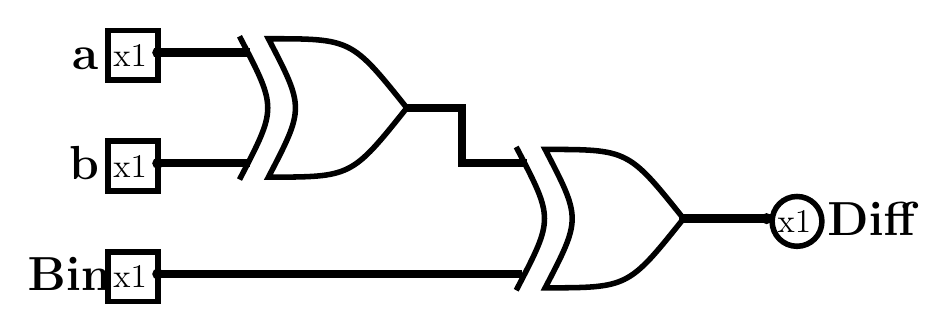
\begin{tikzpicture}[x=1pt,y=-1pt,line cap=rect]
\def\logisimfontA#1{\fontfamily{cmr}{#1}} % Replaced by logisim, original font was "SansSerif"
\definecolor{custcol_0_0_0}{RGB}{0, 0, 0}
\definecolor{custcol_ff_ff_ff}{RGB}{255, 255, 255}
\draw [line width=3.0pt, custcol_0_0_0 ]  (242.0,75.0) -- (272.0,75.0) ;
\draw [line width=3.0pt, custcol_0_0_0 ]  (52.0,15.0) -- (82.0,15.0) -- (84.0,15.0) ;
\draw [line width=3.0pt, custcol_0_0_0 ]  (52.0,55.0) -- (82.0,55.0) -- (84.0,55.0) ;
\draw [line width=2.0pt, custcol_0_0_0 ]  (142.0,35.0) .. controls  (122.0,10.0)  ..  (92.0,10.0) .. controls  (105.0,35.0)  ..  (92.0,60.0) .. controls  (122.0,60.0)  ..  (142.0,35.0) -- cycle ;
\draw [line width=2.0pt, custcol_0_0_0 ]  (82.0,10.0) .. controls  (95.0,35.0)  ..  (82.0,60.0) ;
\draw [line width=2.0pt, custcol_0_0_0]  (283.0,76.0) ellipse (9.0 and 9.0 );
\logisimfontA{\fontsize{12pt}{12pt}\selectfont\node[inner sep=0, outer sep=0, custcol_0_0_0, anchor=base west] at  (276.0,80.0)  {x1};}
\logisimfontA{\fontsize{16pt}{16pt}\fontseries{bx}\selectfont\node[inner sep=0, outer sep=0, custcol_0_0_0, anchor=base west] at  (294.0,81.0)  {Diff};}
\fill [line width=2.0pt, custcol_0_0_0]  (272.0,75.0) ellipse (2.0 and 2.0 );
\draw [line width=3.0pt, custcol_0_0_0 ]  (142.0,35.0) -- (162.0,35.0) -- (162.0,55.0) -- (182.0,55.0) -- (184.0,55.0) ;
\draw [line width=3.0pt, custcol_0_0_0 ]  (52.0,95.0) -- (182.0,95.0) -- (182.0,95.0) ;
\draw [line width=2.0pt, custcol_0_0_0 ]  (242.0,75.0) .. controls  (222.0,50.0)  ..  (192.0,50.0) .. controls  (205.0,75.0)  ..  (192.0,100.0) .. controls  (222.0,100.0)  ..  (242.0,75.0) -- cycle ;
\draw [line width=2.0pt, custcol_0_0_0 ]  (182.0,50.0) .. controls  (195.0,75.0)  ..  (182.0,100.0) ;
\draw [line width=2.0pt, custcol_0_0_0 ]  (34.0,7.0) -- (51.0,7.0) ;
\draw [line width=2.0pt, custcol_0_0_0 ]  (52.0,7.0) -- (52.0,24.0) ;
\draw [line width=2.0pt, custcol_0_0_0 ]  (52.0,25.0) -- (35.0,25.0) ;
\draw [line width=2.0pt, custcol_0_0_0 ]  (34.0,25.0) -- (34.0,8.0) ;
\logisimfontA{\fontsize{12pt}{12pt}\selectfont\node[inner sep=0, outer sep=0, custcol_0_0_0, anchor=base west] at  (36.0,20.0)  {x1};}
\logisimfontA{\fontsize{16pt}{16pt}\fontseries{bx}\selectfont\node[inner sep=0, outer sep=0, custcol_0_0_0, anchor=base west] at  (21.0,21.0)  {a};}
\fill [line width=2.0pt, custcol_0_0_0]  (52.0,15.0) ellipse (2.0 and 2.0 );
\draw [line width=2.0pt, custcol_0_0_0 ]  (34.0,87.0) -- (51.0,87.0) ;
\draw [line width=2.0pt, custcol_0_0_0 ]  (52.0,87.0) -- (52.0,104.0) ;
\draw [line width=2.0pt, custcol_0_0_0 ]  (52.0,105.0) -- (35.0,105.0) ;
\draw [line width=2.0pt, custcol_0_0_0 ]  (34.0,105.0) -- (34.0,88.0) ;
\logisimfontA{\fontsize{12pt}{12pt}\selectfont\node[inner sep=0, outer sep=0, custcol_0_0_0, anchor=base west] at  (36.0,100.0)  {x1};}
\logisimfontA{\fontsize{16pt}{16pt}\fontseries{bx}\selectfont\node[inner sep=0, outer sep=0, custcol_0_0_0, anchor=base west] at  (5.0,101.0)  {Bin};}
\fill [line width=2.0pt, custcol_0_0_0]  (52.0,95.0) ellipse (2.0 and 2.0 );
\draw [line width=2.0pt, custcol_0_0_0 ]  (34.0,47.0) -- (51.0,47.0) ;
\draw [line width=2.0pt, custcol_0_0_0 ]  (52.0,47.0) -- (52.0,64.0) ;
\draw [line width=2.0pt, custcol_0_0_0 ]  (52.0,65.0) -- (35.0,65.0) ;
\draw [line width=2.0pt, custcol_0_0_0 ]  (34.0,65.0) -- (34.0,48.0) ;
\logisimfontA{\fontsize{12pt}{12pt}\selectfont\node[inner sep=0, outer sep=0, custcol_0_0_0, anchor=base west] at  (36.0,60.0)  {x1};}
\logisimfontA{\fontsize{16pt}{16pt}\fontseries{bx}\selectfont\node[inner sep=0, outer sep=0, custcol_0_0_0, anchor=base west] at  (20.0,61.0)  {b};}
\fill [line width=2.0pt, custcol_0_0_0]  (52.0,55.0) ellipse (2.0 and 2.0 );
\end{tikzpicture}
}

			\label{fig:subtratorcompletoparte01}
		\end{figure}
	\end{columns}
\end{frame}
\begin{frame}
	\frametitle{Subtrator completo}
	\framesubtitle{\textbf{Prática dirigida}}
	\par A partir da tabela-verdade mostrada determine a expressão algébrica booleana correspondente e o respectivo circuito de $B_{out}$.
	
	\begin{columns}
		\column{.6\linewidth}
		\begin{table}[h!]
			\centering
			\begin{tabular}{|c|c|c|c|c|}
				\hline
				a & b & $B_{in}$ & Diff & $B_{out}$ \\
				\hline
				0 & 0 & 0 & 0 & 0 \\
				0 & 0 & 1 & 1 & 1 \\
				0 & 1 & 0 & 1 & 1 \\
				0 & 1 & 1 & 0 & 1 \\
				1 & 0 & 0 & 1 & 0 \\
				1 & 0 & 1 & 0 & 0 \\
				1 & 1 & 0 & 0 & 0 \\
				1 & 1 & 1 & 1 & 1 \\
				\hline
			\end{tabular}
			\caption{Tabela-verdade de $B_{out}$ para subtrator completo}
			\label{tab:barroe_out2}
		\end{table}
		\column{.4\linewidth}
			\par Para facilitar a notação considerando $c=B_{in}$ temos por \textit{mimtermos}:
			\begin{equation}
				\begin{aligned}
					&(\overline{a}\overline{b}c)+(\overline{a}b\overline{c})+(\overline{a}bc)+(abc)
				\end{aligned}
			\end{equation}
	\end{columns}
\end{frame}

\begin{frame}
	\frametitle{Subtrator completo}
	\framesubtitle{\textbf{Prática dirigida}}
	\begin{columns}
		\column{.5\linewidth}
		\begin{equation}
			\begin{aligned}
			&(\overline{a}\overline{b}c)+(\overline{a}b\overline{c})+(\overline{a}bc)+(abc) = \\ \pause
			&\text{pondo em evidência } \overline{a}: \\
			&\overline{a}.(\overline{b}c+b\overline{c}+bc)+(abc) =\\  \pause
			&\overline{a}.(\overline{b}c+ b.(\overline{c}+c))+(abc) =\\  \pause
			&\overline{a}.(\overline{b}c+ b.1)+(abc) =\\  \pause
			&\overline{a}.(\overline{b}c+ b)+(abc) =\\  \pause
			&\text{usando o teorema:} x+\overline{x}y = x+y \\
			&\overline{a}.(b+c)+(abc) =\\  \pause
			&\overline{a}b+\overline{a}c+abc =\\
			\end{aligned}
		\end{equation}
		\column{.5\linewidth}
		\begin{equation}
			\begin{aligned}
				&\overline{a}b+\overline{a}c+abc =\\  \pause
				&\text{fatorando } c: \\
				&\overline{a}b+c.(\overline{a}+ab) = \\  \pause
				&\text{usando o teorema:} x+\overline{x}y = x+y \\
				&\overline{a}b+c.(\overline{a}+b) = \\  \pause
				&\overline{a}b+\overline{a}c+bc \therefore \\ 
				&\boxed{B_{out}=\overline{a}b+\overline{a}B_{in}+bB_{in}}
			\end{aligned}
		\end{equation}
	\end{columns}
\end{frame}

\begin{frame}
	\frametitle{Subtrator completo}
	\framesubtitle{\textbf{Prática dirigida}}
	\par Portanto o circuito do $B_{out}$ fica assim:
	\begin{figure}
		\centering
		% Important: If latex complains about unicode characters,
% please use "\usepackage[utf8x]{inputenc}" in your preamble
% You can change the size of the picture by putting it into the construct:
% 1) \resizebox{10cm}{!}{"below picture"} to scale horizontally to 10 cm
% 2) \resizebox{!}{15cm}{"below picture"} to scale vertically to 15 cm
% 3) \resizebox{10cm}{15cm}{"below picture"} a combination of above two
% It is not recomended to use the scale option of the tikzpicture environment.
\resizebox{10cm}{!}{
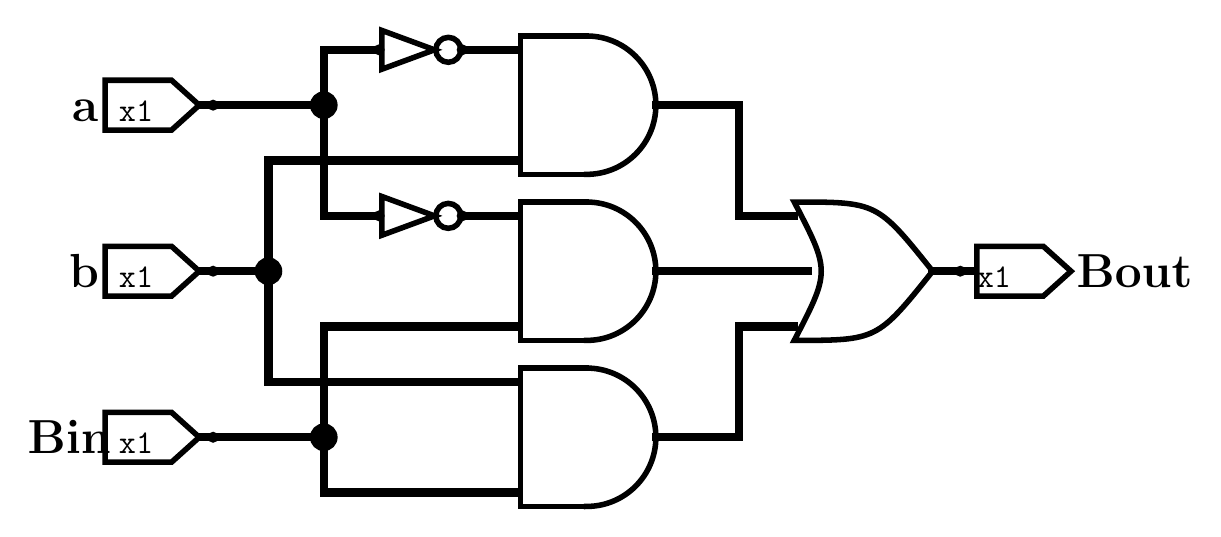
\begin{tikzpicture}[x=1pt,y=-1pt,line cap=rect]
\def\logisimfontA#1{\fontfamily{cmr}{#1}} % Replaced by logisim, original font was "SansSerif"
\def\logisimfontB#1{\fontfamily{cmtt}{#1}} % Replaced by logisim, original font was "Monospaced"
\definecolor{custcol_0_0_0}{RGB}{0, 0, 0}
\definecolor{custcol_ff_ff_ff}{RGB}{255, 255, 255}
\draw [line width=3.0pt, custcol_0_0_0 ]  (162.0,14.0) -- (182.0,14.0) ;
\draw [line width=3.0pt, custcol_0_0_0 ]  (162.0,74.0) -- (182.0,74.0) ;
\draw [line width=3.0pt, custcol_0_0_0 ]  (182.0,54.0) -- (92.0,54.0) -- (92.0,94.0) ;
\draw [line width=3.0pt, custcol_0_0_0 ]  (112.0,34.0) -- (112.0,74.0) -- (132.0,74.0) ;
\draw [line width=3.0pt, custcol_0_0_0 ]  (332.0,94.0) -- (342.0,94.0) ;
\draw [line width=3.0pt, custcol_0_0_0 ]  (112.0,154.0) -- (112.0,114.0) -- (182.0,114.0) ;
\fill [line width=3.0pt, custcol_0_0_0]  (112.0,154.0) ellipse (5.0 and 5.0 );
\fill [line width=3.0pt, custcol_0_0_0]  (112.0,34.0) ellipse (5.0 and 5.0 );
\fill [line width=3.0pt, custcol_0_0_0]  (92.0,94.0) ellipse (5.0 and 5.0 );
\draw [line width=2.0pt, custcol_0_0_0] (207.0,119.0) arc (90.0:-90.0:25.0 and 25.0 );
\draw [line width=2.0pt, custcol_0_0_0 ]  (207.0,69.0) -- (183.0,69.0) -- (183.0,119.0) -- (207.0,119.0) ;
\draw [line width=2.0pt, custcol_0_0_0] (207.0,179.0) arc (90.0:-90.0:25.0 and 25.0 );
\draw [line width=2.0pt, custcol_0_0_0 ]  (207.0,129.0) -- (183.0,129.0) -- (183.0,179.0) -- (207.0,179.0) ;
\draw [line width=2.0pt, custcol_0_0_0] (207.0,59.0) arc (90.0:-90.0:25.0 and 25.0 );
\draw [line width=2.0pt, custcol_0_0_0 ]  (207.0,9.0) -- (183.0,9.0) -- (183.0,59.0) -- (207.0,59.0) ;
\draw [line width=3.0pt, custcol_0_0_0 ]  (232.0,34.0) -- (262.0,34.0) -- (262.0,74.0) -- (282.0,74.0) -- (282.0,74.0) ;
\draw [line width=3.0pt, custcol_0_0_0 ]  (232.0,94.0) -- (282.0,94.0) -- (287.0,94.0) ;
\draw [line width=3.0pt, custcol_0_0_0 ]  (282.0,114.0) -- (282.0,114.0) -- (262.0,114.0) -- (262.0,154.0) -- (232.0,154.0) ;
\draw [line width=2.0pt, custcol_0_0_0 ]  (332.0,94.0) .. controls  (312.0,69.0)  ..  (282.0,69.0) .. controls  (295.0,94.0)  ..  (282.0,119.0) .. controls  (312.0,119.0)  ..  (332.0,94.0) -- cycle ;
\draw [line width=3.0pt, custcol_0_0_0 ]  (346.0,94.0) -- (343.0,94.0) ;
\draw [line width=2.0pt, custcol_0_0_0 ]  (372.0,85.0) -- (382.0,94.0) -- (372.0,103.0) -- (348.0,103.0) -- (348.0,85.0) -- cycle;
\logisimfontB{\fontsize{12pt}{12pt}\selectfont\node[inner sep=0, outer sep=0, custcol_0_0_0, anchor=base west] at  (348.0,100.0)  {x1};}
\logisimfontA{\fontsize{16pt}{16pt}\fontseries{bx}\selectfont\node[inner sep=0, outer sep=0, custcol_0_0_0, anchor=base west] at  (384.0,100.0)  {Bout};}
\fill [line width=2.0pt, custcol_0_0_0]  (342.0,94.0) ellipse (2.0 and 2.0 );
\draw [line width=2.0pt, custcol_0_0_0 ]  (152.0,14.0) -- (133.0,7.0) -- (133.0,21.0) -- cycle;
\draw [line width=2.0pt, custcol_0_0_0]  (157.0,14.0) ellipse (4.5 and 4.5 );
\fill [line width=2.0pt, custcol_0_0_0]  (162.0,14.0) ellipse (2.0 and 2.0 );
\fill [line width=2.0pt, custcol_0_0_0]  (132.0,14.0) ellipse (2.0 and 2.0 );
\draw [line width=2.0pt, custcol_0_0_0 ]  (152.0,74.0) -- (133.0,67.0) -- (133.0,81.0) -- cycle;
\draw [line width=2.0pt, custcol_0_0_0]  (157.0,74.0) ellipse (4.5 and 4.5 );
\fill [line width=2.0pt, custcol_0_0_0]  (162.0,74.0) ellipse (2.0 and 2.0 );
\fill [line width=2.0pt, custcol_0_0_0]  (132.0,74.0) ellipse (2.0 and 2.0 );
\draw [line width=3.0pt, custcol_0_0_0 ]  (67.0,154.0) -- (72.0,154.0) -- (112.0,154.0) -- (112.0,174.0) -- (182.0,174.0) ;
\draw [line width=2.0pt, custcol_0_0_0 ]  (57.0,163.0) -- (67.0,154.0) -- (57.0,145.0) -- (33.0,145.0) -- (33.0,163.0) -- cycle;
\logisimfontB{\fontsize{12pt}{12pt}\selectfont\node[inner sep=0, outer sep=0, custcol_0_0_0, anchor=base west] at  (38.0,160.0)  {x1};}
\logisimfontA{\fontsize{16pt}{16pt}\fontseries{bx}\selectfont\node[inner sep=0, outer sep=0, custcol_0_0_0, anchor=base west] at  (5.0,160.0)  {Bin};}
\fill [line width=2.0pt, custcol_0_0_0]  (72.0,154.0) ellipse (2.0 and 2.0 );
\draw [line width=3.0pt, custcol_0_0_0 ]  (67.0,94.0) -- (72.0,94.0) -- (92.0,94.0) -- (92.0,134.0) -- (182.0,134.0) ;
\draw [line width=2.0pt, custcol_0_0_0 ]  (57.0,103.0) -- (67.0,94.0) -- (57.0,85.0) -- (33.0,85.0) -- (33.0,103.0) -- cycle;
\logisimfontB{\fontsize{12pt}{12pt}\selectfont\node[inner sep=0, outer sep=0, custcol_0_0_0, anchor=base west] at  (38.0,100.0)  {x1};}
\logisimfontA{\fontsize{16pt}{16pt}\fontseries{bx}\selectfont\node[inner sep=0, outer sep=0, custcol_0_0_0, anchor=base west] at  (20.0,100.0)  {b};}
\fill [line width=2.0pt, custcol_0_0_0]  (72.0,94.0) ellipse (2.0 and 2.0 );
\draw [line width=3.0pt, custcol_0_0_0 ]  (67.0,34.0) -- (72.0,34.0) -- (112.0,34.0) -- (112.0,14.0) -- (132.0,14.0) ;
\draw [line width=2.0pt, custcol_0_0_0 ]  (57.0,43.0) -- (67.0,34.0) -- (57.0,25.0) -- (33.0,25.0) -- (33.0,43.0) -- cycle;
\logisimfontB{\fontsize{12pt}{12pt}\selectfont\node[inner sep=0, outer sep=0, custcol_0_0_0, anchor=base west] at  (38.0,40.0)  {x1};}
\logisimfontA{\fontsize{16pt}{16pt}\fontseries{bx}\selectfont\node[inner sep=0, outer sep=0, custcol_0_0_0, anchor=base west] at  (21.0,40.0)  {a};}
\fill [line width=2.0pt, custcol_0_0_0]  (72.0,34.0) ellipse (2.0 and 2.0 );
\end{tikzpicture}
}

		\label{fig:subtratorcompletoparte02}
	\end{figure}
\end{frame}

\begin{frame}
	\frametitle{Subtrator completo}
	\framesubtitle{\textbf{Prática dirigida}}
	\par Portanto o circuito \textbf{subtrator completo} ou \textbf{Full subtractor} fica assim:
	\begin{figure}
		\centering
		% Important: If latex complains about unicode characters,
% please use "\usepackage[utf8x]{inputenc}" in your preamble
% You can change the size of the picture by putting it into the construct:
% 1) \resizebox{10cm}{!}{"below picture"} to scale horizontally to 10 cm
% 2) \resizebox{!}{15cm}{"below picture"} to scale vertically to 15 cm
% 3) \resizebox{10cm}{15cm}{"below picture"} a combination of above two
% It is not recomended to use the scale option of the tikzpicture environment.
 \resizebox{7cm}{!}{
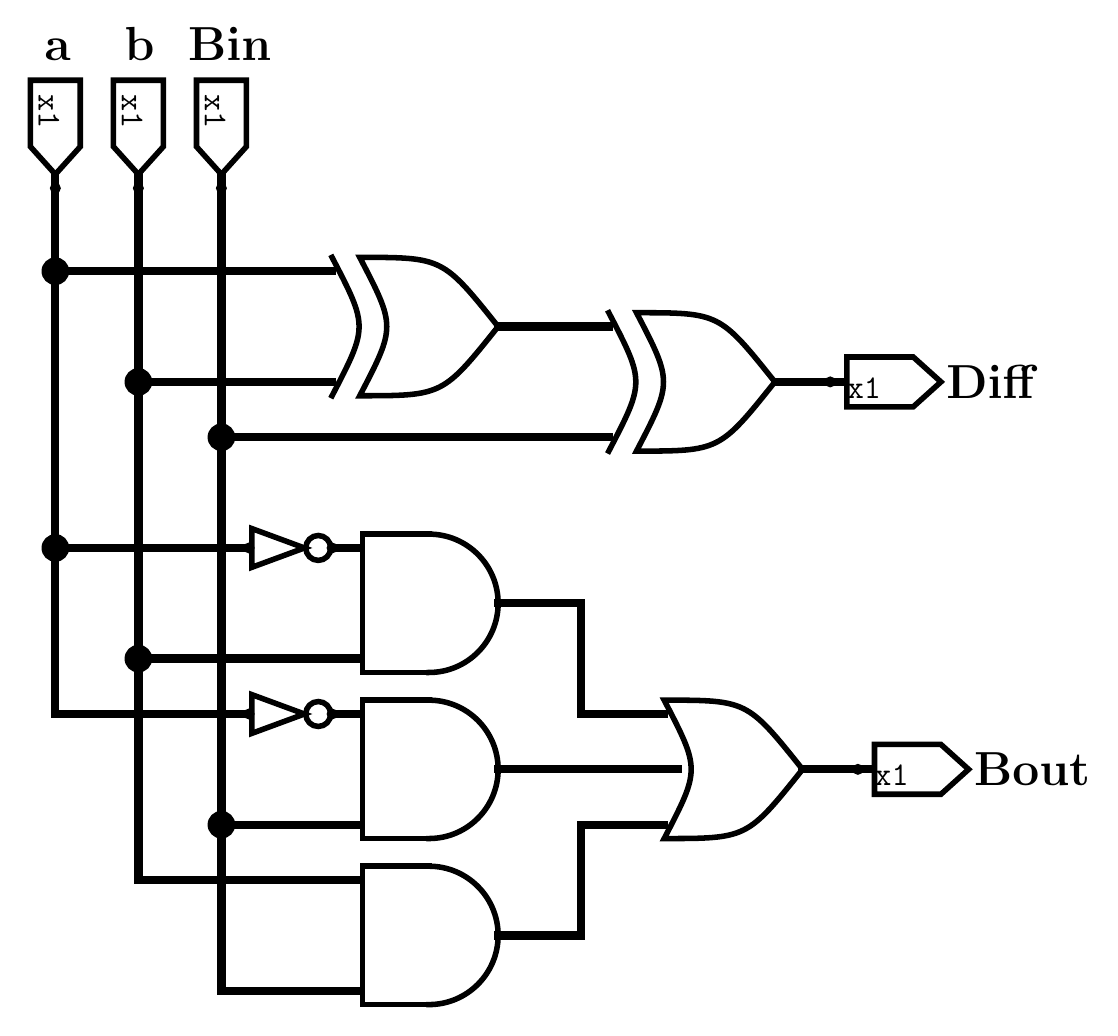
\begin{tikzpicture}[x=1pt,y=-1pt,line cap=rect]
\def\logisimfontA#1{\fontfamily{cmr}{#1}} % Replaced by logisim, original font was "SansSerif"
\def\logisimfontB#1{\fontfamily{cmtt}{#1}} % Replaced by logisim, original font was "Monospaced"
\definecolor{custcol_0_0_0}{RGB}{0, 0, 0}
\definecolor{custcol_ff_ff_ff}{RGB}{255, 255, 255}
\draw [line width=3.0pt, custcol_0_0_0 ]  (275.0,134.0) -- (295.0,134.0) ;
\draw [line width=3.0pt, custcol_0_0_0 ]  (285.0,274.0) -- (305.0,274.0) ;
\draw [line width=3.0pt, custcol_0_0_0 ]  (115.0,254.0) -- (125.0,254.0) ;
\draw [line width=3.0pt, custcol_0_0_0 ]  (115.0,194.0) -- (125.0,194.0) ;
\draw [line width=3.0pt, custcol_0_0_0 ]  (45.0,234.0) -- (125.0,234.0) ;
\draw [line width=3.0pt, custcol_0_0_0 ]  (75.0,294.0) -- (75.0,354.0) -- (125.0,354.0) ;
\draw [line width=3.0pt, custcol_0_0_0 ]  (15.0,194.0) -- (85.0,194.0) ;
\draw [line width=3.0pt, custcol_0_0_0 ]  (15.0,94.0) -- (15.0,194.0) -- (15.0,254.0) -- (85.0,254.0) ;
\fill [line width=3.0pt, custcol_0_0_0]  (45.0,134.0) ellipse (5.0 and 5.0 );
\fill [line width=3.0pt, custcol_0_0_0]  (75.0,294.0) ellipse (5.0 and 5.0 );
\fill [line width=3.0pt, custcol_0_0_0]  (15.0,194.0) ellipse (5.0 and 5.0 );
\fill [line width=3.0pt, custcol_0_0_0]  (45.0,234.0) ellipse (5.0 and 5.0 );
\fill [line width=3.0pt, custcol_0_0_0]  (15.0,94.0) ellipse (5.0 and 5.0 );
\fill [line width=3.0pt, custcol_0_0_0]  (75.0,154.0) ellipse (5.0 and 5.0 );
\draw [line width=2.0pt, custcol_0_0_0 ]  (6.0,49.0) -- (15.0,59.0) -- (24.0,49.0) -- (24.0,25.0) -- (6.0,25.0) -- cycle;
\logisimfontB{\fontsize{12pt}{12pt}\selectfont\node[inner sep=0, outer sep=0, custcol_0_0_0, anchor=base west, rotate=-90.0] at  (9.0,30.0)  {x1};}
\logisimfontA{\fontsize{16pt}{16pt}\fontseries{bx}\selectfont\node[inner sep=0, outer sep=0, custcol_0_0_0, anchor=base west] at  (11.0,18.0)  {a};}
\fill [line width=2.0pt, custcol_0_0_0]  (15.0,64.0) ellipse (2.0 and 2.0 );
\draw [line width=3.0pt, custcol_0_0_0 ]  (45.0,59.0) -- (45.0,64.0) -- (45.0,134.0) -- (45.0,234.0) -- (45.0,314.0) -- (125.0,314.0) ;
\draw [line width=2.0pt, custcol_0_0_0 ]  (36.0,49.0) -- (45.0,59.0) -- (54.0,49.0) -- (54.0,25.0) -- (36.0,25.0) -- cycle;
\logisimfontB{\fontsize{12pt}{12pt}\selectfont\node[inner sep=0, outer sep=0, custcol_0_0_0, anchor=base west, rotate=-90.0] at  (39.0,30.0)  {x1};}
\logisimfontA{\fontsize{16pt}{16pt}\fontseries{bx}\selectfont\node[inner sep=0, outer sep=0, custcol_0_0_0, anchor=base west] at  (40.0,18.0)  {b};}
\fill [line width=2.0pt, custcol_0_0_0]  (45.0,64.0) ellipse (2.0 and 2.0 );
\draw [line width=3.0pt, custcol_0_0_0 ]  (75.0,59.0) -- (75.0,64.0) -- (75.0,154.0) -- (75.0,294.0) -- (125.0,294.0) ;
\draw [line width=2.0pt, custcol_0_0_0 ]  (66.0,49.0) -- (75.0,59.0) -- (84.0,49.0) -- (84.0,25.0) -- (66.0,25.0) -- cycle;
\logisimfontB{\fontsize{12pt}{12pt}\selectfont\node[inner sep=0, outer sep=0, custcol_0_0_0, anchor=base west, rotate=-90.0] at  (69.0,30.0)  {x1};}
\logisimfontA{\fontsize{16pt}{16pt}\fontseries{bx}\selectfont\node[inner sep=0, outer sep=0, custcol_0_0_0, anchor=base west] at  (63.0,18.0)  {Bin};}
\fill [line width=2.0pt, custcol_0_0_0]  (75.0,64.0) ellipse (2.0 and 2.0 );
\draw [line width=3.0pt, custcol_0_0_0 ]  (299.0,134.0) -- (296.0,134.0) ;
\draw [line width=2.0pt, custcol_0_0_0 ]  (325.0,125.0) -- (335.0,134.0) -- (325.0,143.0) -- (301.0,143.0) -- (301.0,125.0) -- cycle;
\logisimfontB{\fontsize{12pt}{12pt}\selectfont\node[inner sep=0, outer sep=0, custcol_0_0_0, anchor=base west] at  (301.0,140.0)  {x1};}
\logisimfontA{\fontsize{16pt}{16pt}\fontseries{bx}\selectfont\node[inner sep=0, outer sep=0, custcol_0_0_0, anchor=base west] at  (337.0,140.0)  {Diff};}
\fill [line width=2.0pt, custcol_0_0_0]  (295.0,134.0) ellipse (2.0 and 2.0 );
\draw [line width=3.0pt, custcol_0_0_0 ]  (15.0,59.0) -- (15.0,64.0) -- (15.0,94.0) -- (115.0,94.0) -- (115.0,94.0) ;
\draw [line width=3.0pt, custcol_0_0_0 ]  (45.0,134.0) -- (115.0,134.0) -- (115.0,134.0) ;
\draw [line width=2.0pt, custcol_0_0_0 ]  (175.0,114.0) .. controls  (155.0,89.0)  ..  (125.0,89.0) .. controls  (138.0,114.0)  ..  (125.0,139.0) .. controls  (155.0,139.0)  ..  (175.0,114.0) -- cycle ;
\draw [line width=2.0pt, custcol_0_0_0 ]  (115.0,89.0) .. controls  (128.0,114.0)  ..  (115.0,139.0) ;
\draw [line width=3.0pt, custcol_0_0_0 ]  (175.0,114.0) -- (215.0,114.0) -- (215.0,114.0) ;
\draw [line width=3.0pt, custcol_0_0_0 ]  (75.0,154.0) -- (215.0,154.0) -- (215.0,154.0) ;
\draw [line width=2.0pt, custcol_0_0_0 ]  (275.0,134.0) .. controls  (255.0,109.0)  ..  (225.0,109.0) .. controls  (238.0,134.0)  ..  (225.0,159.0) .. controls  (255.0,159.0)  ..  (275.0,134.0) -- cycle ;
\draw [line width=2.0pt, custcol_0_0_0 ]  (215.0,109.0) .. controls  (228.0,134.0)  ..  (215.0,159.0) ;
\draw [line width=2.0pt, custcol_0_0_0 ]  (105.0,194.0) -- (86.0,187.0) -- (86.0,201.0) -- cycle;
\draw [line width=2.0pt, custcol_0_0_0]  (110.0,194.0) ellipse (4.5 and 4.5 );
\fill [line width=2.0pt, custcol_0_0_0]  (115.0,194.0) ellipse (2.0 and 2.0 );
\fill [line width=2.0pt, custcol_0_0_0]  (85.0,194.0) ellipse (2.0 and 2.0 );
\draw [line width=3.0pt, custcol_0_0_0 ]  (309.0,274.0) -- (306.0,274.0) ;
\draw [line width=2.0pt, custcol_0_0_0 ]  (335.0,265.0) -- (345.0,274.0) -- (335.0,283.0) -- (311.0,283.0) -- (311.0,265.0) -- cycle;
\logisimfontB{\fontsize{12pt}{12pt}\selectfont\node[inner sep=0, outer sep=0, custcol_0_0_0, anchor=base west] at  (311.0,280.0)  {x1};}
\logisimfontA{\fontsize{16pt}{16pt}\fontseries{bx}\selectfont\node[inner sep=0, outer sep=0, custcol_0_0_0, anchor=base west] at  (347.0,280.0)  {Bout};}
\fill [line width=2.0pt, custcol_0_0_0]  (305.0,274.0) ellipse (2.0 and 2.0 );
\draw [line width=2.0pt, custcol_0_0_0] (150.0,239.0) arc (90.0:-90.0:25.0 and 25.0 );
\draw [line width=2.0pt, custcol_0_0_0 ]  (150.0,189.0) -- (126.0,189.0) -- (126.0,239.0) -- (150.0,239.0) ;
\draw [line width=2.0pt, custcol_0_0_0] (150.0,359.0) arc (90.0:-90.0:25.0 and 25.0 );
\draw [line width=2.0pt, custcol_0_0_0 ]  (150.0,309.0) -- (126.0,309.0) -- (126.0,359.0) -- (150.0,359.0) ;
\draw [line width=2.0pt, custcol_0_0_0] (150.0,299.0) arc (90.0:-90.0:25.0 and 25.0 );
\draw [line width=2.0pt, custcol_0_0_0 ]  (150.0,249.0) -- (126.0,249.0) -- (126.0,299.0) -- (150.0,299.0) ;
\draw [line width=3.0pt, custcol_0_0_0 ]  (175.0,214.0) -- (205.0,214.0) -- (205.0,254.0) -- (235.0,254.0) -- (235.0,254.0) ;
\draw [line width=3.0pt, custcol_0_0_0 ]  (175.0,274.0) -- (235.0,274.0) -- (240.0,274.0) ;
\draw [line width=3.0pt, custcol_0_0_0 ]  (235.0,294.0) -- (235.0,294.0) -- (205.0,294.0) -- (205.0,334.0) -- (175.0,334.0) ;
\draw [line width=2.0pt, custcol_0_0_0 ]  (285.0,274.0) .. controls  (265.0,249.0)  ..  (235.0,249.0) .. controls  (248.0,274.0)  ..  (235.0,299.0) .. controls  (265.0,299.0)  ..  (285.0,274.0) -- cycle ;
\draw [line width=2.0pt, custcol_0_0_0 ]  (105.0,254.0) -- (86.0,247.0) -- (86.0,261.0) -- cycle;
\draw [line width=2.0pt, custcol_0_0_0]  (110.0,254.0) ellipse (4.5 and 4.5 );
\fill [line width=2.0pt, custcol_0_0_0]  (115.0,254.0) ellipse (2.0 and 2.0 );
\fill [line width=2.0pt, custcol_0_0_0]  (85.0,254.0) ellipse (2.0 and 2.0 );
\end{tikzpicture}
}

		\label{fig:subtratorcompleto}
	\end{figure}
\end{frame}

\section{Mas... mas... \textit{Oh... wait a fucking moment!}}

\begin{frame}
	\frametitle{KKKKKKKK}
	\begin{columns}
		\column{.5\linewidth}
			\begin{figure}
			\centering
			% Important: If latex complains about unicode characters,
% please use "\usepackage[utf8x]{inputenc}" in your preamble
% You can change the size of the picture by putting it into the construct:
% 1) \resizebox{10cm}{!}{"below picture"} to scale horizontally to 10 cm
% 2) \resizebox{!}{15cm}{"below picture"} to scale vertically to 15 cm
% 3) \resizebox{10cm}{15cm}{"below picture"} a combination of above two
% It is not recomended to use the scale option of the tikzpicture environment.
 \resizebox{7cm}{!}{
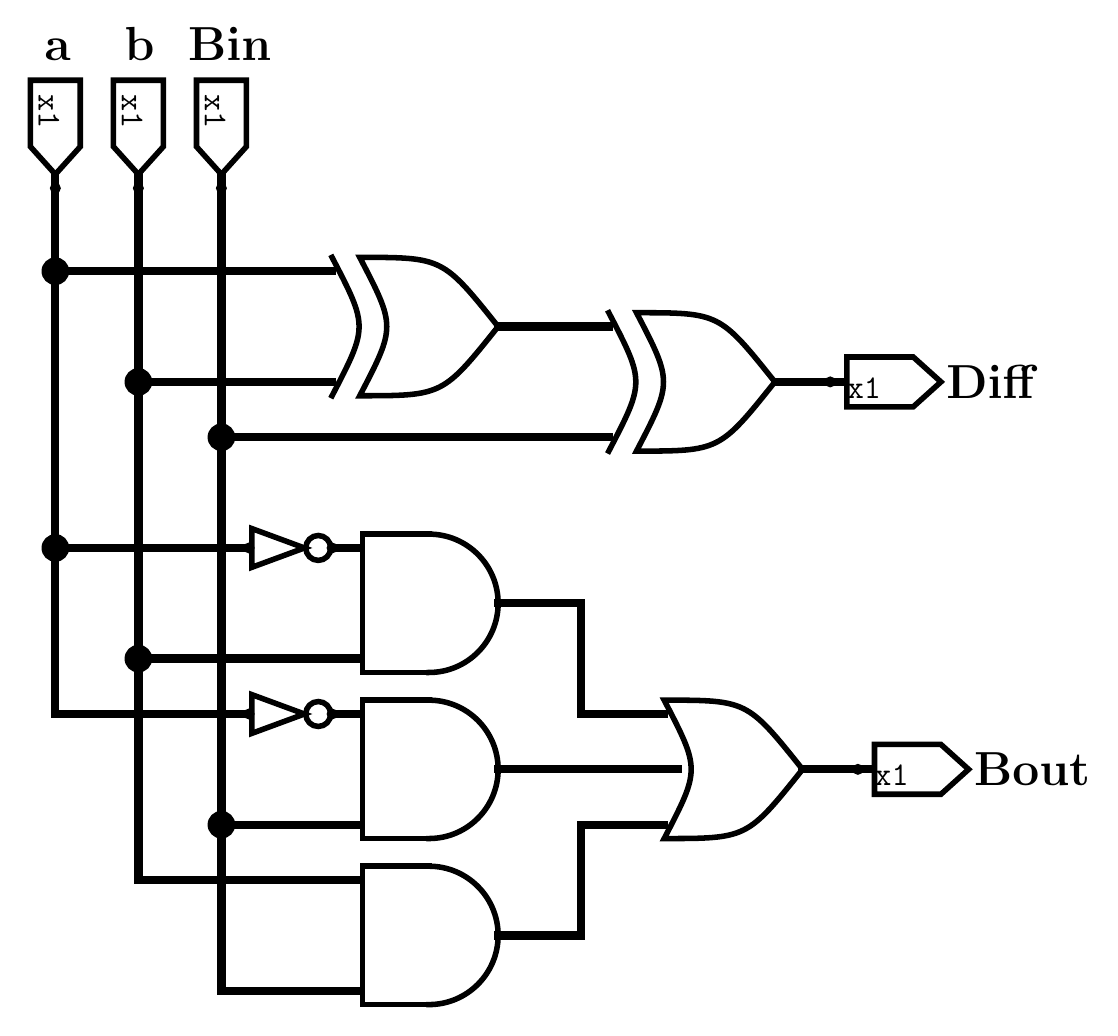
\begin{tikzpicture}[x=1pt,y=-1pt,line cap=rect]
\def\logisimfontA#1{\fontfamily{cmr}{#1}} % Replaced by logisim, original font was "SansSerif"
\def\logisimfontB#1{\fontfamily{cmtt}{#1}} % Replaced by logisim, original font was "Monospaced"
\definecolor{custcol_0_0_0}{RGB}{0, 0, 0}
\definecolor{custcol_ff_ff_ff}{RGB}{255, 255, 255}
\draw [line width=3.0pt, custcol_0_0_0 ]  (275.0,134.0) -- (295.0,134.0) ;
\draw [line width=3.0pt, custcol_0_0_0 ]  (285.0,274.0) -- (305.0,274.0) ;
\draw [line width=3.0pt, custcol_0_0_0 ]  (115.0,254.0) -- (125.0,254.0) ;
\draw [line width=3.0pt, custcol_0_0_0 ]  (115.0,194.0) -- (125.0,194.0) ;
\draw [line width=3.0pt, custcol_0_0_0 ]  (45.0,234.0) -- (125.0,234.0) ;
\draw [line width=3.0pt, custcol_0_0_0 ]  (75.0,294.0) -- (75.0,354.0) -- (125.0,354.0) ;
\draw [line width=3.0pt, custcol_0_0_0 ]  (15.0,194.0) -- (85.0,194.0) ;
\draw [line width=3.0pt, custcol_0_0_0 ]  (15.0,94.0) -- (15.0,194.0) -- (15.0,254.0) -- (85.0,254.0) ;
\fill [line width=3.0pt, custcol_0_0_0]  (45.0,134.0) ellipse (5.0 and 5.0 );
\fill [line width=3.0pt, custcol_0_0_0]  (75.0,294.0) ellipse (5.0 and 5.0 );
\fill [line width=3.0pt, custcol_0_0_0]  (15.0,194.0) ellipse (5.0 and 5.0 );
\fill [line width=3.0pt, custcol_0_0_0]  (45.0,234.0) ellipse (5.0 and 5.0 );
\fill [line width=3.0pt, custcol_0_0_0]  (15.0,94.0) ellipse (5.0 and 5.0 );
\fill [line width=3.0pt, custcol_0_0_0]  (75.0,154.0) ellipse (5.0 and 5.0 );
\draw [line width=2.0pt, custcol_0_0_0 ]  (6.0,49.0) -- (15.0,59.0) -- (24.0,49.0) -- (24.0,25.0) -- (6.0,25.0) -- cycle;
\logisimfontB{\fontsize{12pt}{12pt}\selectfont\node[inner sep=0, outer sep=0, custcol_0_0_0, anchor=base west, rotate=-90.0] at  (9.0,30.0)  {x1};}
\logisimfontA{\fontsize{16pt}{16pt}\fontseries{bx}\selectfont\node[inner sep=0, outer sep=0, custcol_0_0_0, anchor=base west] at  (11.0,18.0)  {a};}
\fill [line width=2.0pt, custcol_0_0_0]  (15.0,64.0) ellipse (2.0 and 2.0 );
\draw [line width=3.0pt, custcol_0_0_0 ]  (45.0,59.0) -- (45.0,64.0) -- (45.0,134.0) -- (45.0,234.0) -- (45.0,314.0) -- (125.0,314.0) ;
\draw [line width=2.0pt, custcol_0_0_0 ]  (36.0,49.0) -- (45.0,59.0) -- (54.0,49.0) -- (54.0,25.0) -- (36.0,25.0) -- cycle;
\logisimfontB{\fontsize{12pt}{12pt}\selectfont\node[inner sep=0, outer sep=0, custcol_0_0_0, anchor=base west, rotate=-90.0] at  (39.0,30.0)  {x1};}
\logisimfontA{\fontsize{16pt}{16pt}\fontseries{bx}\selectfont\node[inner sep=0, outer sep=0, custcol_0_0_0, anchor=base west] at  (40.0,18.0)  {b};}
\fill [line width=2.0pt, custcol_0_0_0]  (45.0,64.0) ellipse (2.0 and 2.0 );
\draw [line width=3.0pt, custcol_0_0_0 ]  (75.0,59.0) -- (75.0,64.0) -- (75.0,154.0) -- (75.0,294.0) -- (125.0,294.0) ;
\draw [line width=2.0pt, custcol_0_0_0 ]  (66.0,49.0) -- (75.0,59.0) -- (84.0,49.0) -- (84.0,25.0) -- (66.0,25.0) -- cycle;
\logisimfontB{\fontsize{12pt}{12pt}\selectfont\node[inner sep=0, outer sep=0, custcol_0_0_0, anchor=base west, rotate=-90.0] at  (69.0,30.0)  {x1};}
\logisimfontA{\fontsize{16pt}{16pt}\fontseries{bx}\selectfont\node[inner sep=0, outer sep=0, custcol_0_0_0, anchor=base west] at  (63.0,18.0)  {Bin};}
\fill [line width=2.0pt, custcol_0_0_0]  (75.0,64.0) ellipse (2.0 and 2.0 );
\draw [line width=3.0pt, custcol_0_0_0 ]  (299.0,134.0) -- (296.0,134.0) ;
\draw [line width=2.0pt, custcol_0_0_0 ]  (325.0,125.0) -- (335.0,134.0) -- (325.0,143.0) -- (301.0,143.0) -- (301.0,125.0) -- cycle;
\logisimfontB{\fontsize{12pt}{12pt}\selectfont\node[inner sep=0, outer sep=0, custcol_0_0_0, anchor=base west] at  (301.0,140.0)  {x1};}
\logisimfontA{\fontsize{16pt}{16pt}\fontseries{bx}\selectfont\node[inner sep=0, outer sep=0, custcol_0_0_0, anchor=base west] at  (337.0,140.0)  {Diff};}
\fill [line width=2.0pt, custcol_0_0_0]  (295.0,134.0) ellipse (2.0 and 2.0 );
\draw [line width=3.0pt, custcol_0_0_0 ]  (15.0,59.0) -- (15.0,64.0) -- (15.0,94.0) -- (115.0,94.0) -- (115.0,94.0) ;
\draw [line width=3.0pt, custcol_0_0_0 ]  (45.0,134.0) -- (115.0,134.0) -- (115.0,134.0) ;
\draw [line width=2.0pt, custcol_0_0_0 ]  (175.0,114.0) .. controls  (155.0,89.0)  ..  (125.0,89.0) .. controls  (138.0,114.0)  ..  (125.0,139.0) .. controls  (155.0,139.0)  ..  (175.0,114.0) -- cycle ;
\draw [line width=2.0pt, custcol_0_0_0 ]  (115.0,89.0) .. controls  (128.0,114.0)  ..  (115.0,139.0) ;
\draw [line width=3.0pt, custcol_0_0_0 ]  (175.0,114.0) -- (215.0,114.0) -- (215.0,114.0) ;
\draw [line width=3.0pt, custcol_0_0_0 ]  (75.0,154.0) -- (215.0,154.0) -- (215.0,154.0) ;
\draw [line width=2.0pt, custcol_0_0_0 ]  (275.0,134.0) .. controls  (255.0,109.0)  ..  (225.0,109.0) .. controls  (238.0,134.0)  ..  (225.0,159.0) .. controls  (255.0,159.0)  ..  (275.0,134.0) -- cycle ;
\draw [line width=2.0pt, custcol_0_0_0 ]  (215.0,109.0) .. controls  (228.0,134.0)  ..  (215.0,159.0) ;
\draw [line width=2.0pt, custcol_0_0_0 ]  (105.0,194.0) -- (86.0,187.0) -- (86.0,201.0) -- cycle;
\draw [line width=2.0pt, custcol_0_0_0]  (110.0,194.0) ellipse (4.5 and 4.5 );
\fill [line width=2.0pt, custcol_0_0_0]  (115.0,194.0) ellipse (2.0 and 2.0 );
\fill [line width=2.0pt, custcol_0_0_0]  (85.0,194.0) ellipse (2.0 and 2.0 );
\draw [line width=3.0pt, custcol_0_0_0 ]  (309.0,274.0) -- (306.0,274.0) ;
\draw [line width=2.0pt, custcol_0_0_0 ]  (335.0,265.0) -- (345.0,274.0) -- (335.0,283.0) -- (311.0,283.0) -- (311.0,265.0) -- cycle;
\logisimfontB{\fontsize{12pt}{12pt}\selectfont\node[inner sep=0, outer sep=0, custcol_0_0_0, anchor=base west] at  (311.0,280.0)  {x1};}
\logisimfontA{\fontsize{16pt}{16pt}\fontseries{bx}\selectfont\node[inner sep=0, outer sep=0, custcol_0_0_0, anchor=base west] at  (347.0,280.0)  {Bout};}
\fill [line width=2.0pt, custcol_0_0_0]  (305.0,274.0) ellipse (2.0 and 2.0 );
\draw [line width=2.0pt, custcol_0_0_0] (150.0,239.0) arc (90.0:-90.0:25.0 and 25.0 );
\draw [line width=2.0pt, custcol_0_0_0 ]  (150.0,189.0) -- (126.0,189.0) -- (126.0,239.0) -- (150.0,239.0) ;
\draw [line width=2.0pt, custcol_0_0_0] (150.0,359.0) arc (90.0:-90.0:25.0 and 25.0 );
\draw [line width=2.0pt, custcol_0_0_0 ]  (150.0,309.0) -- (126.0,309.0) -- (126.0,359.0) -- (150.0,359.0) ;
\draw [line width=2.0pt, custcol_0_0_0] (150.0,299.0) arc (90.0:-90.0:25.0 and 25.0 );
\draw [line width=2.0pt, custcol_0_0_0 ]  (150.0,249.0) -- (126.0,249.0) -- (126.0,299.0) -- (150.0,299.0) ;
\draw [line width=3.0pt, custcol_0_0_0 ]  (175.0,214.0) -- (205.0,214.0) -- (205.0,254.0) -- (235.0,254.0) -- (235.0,254.0) ;
\draw [line width=3.0pt, custcol_0_0_0 ]  (175.0,274.0) -- (235.0,274.0) -- (240.0,274.0) ;
\draw [line width=3.0pt, custcol_0_0_0 ]  (235.0,294.0) -- (235.0,294.0) -- (205.0,294.0) -- (205.0,334.0) -- (175.0,334.0) ;
\draw [line width=2.0pt, custcol_0_0_0 ]  (285.0,274.0) .. controls  (265.0,249.0)  ..  (235.0,249.0) .. controls  (248.0,274.0)  ..  (235.0,299.0) .. controls  (265.0,299.0)  ..  (285.0,274.0) -- cycle ;
\draw [line width=2.0pt, custcol_0_0_0 ]  (105.0,254.0) -- (86.0,247.0) -- (86.0,261.0) -- cycle;
\draw [line width=2.0pt, custcol_0_0_0]  (110.0,254.0) ellipse (4.5 and 4.5 );
\fill [line width=2.0pt, custcol_0_0_0]  (115.0,254.0) ellipse (2.0 and 2.0 );
\fill [line width=2.0pt, custcol_0_0_0]  (85.0,254.0) ellipse (2.0 and 2.0 );
\end{tikzpicture}
}

			\label{fig:subtratorcompleto2}
		\end{figure}
		\column{.5\linewidth}
			\begin{figure}
			\centering
			% Important: If latex complains about unicode characters,
% please use "\usepackage[utf8x]{inputenc}" in your preamble
% You can change the size of the picture by putting it into the construct:
% 1) \resizebox{10cm}{!}{"below picture"} to scale horizontally to 10 cm
% 2) \resizebox{!}{15cm}{"below picture"} to scale vertically to 15 cm
% 3) \resizebox{10cm}{15cm}{"below picture"} a combination of above two
% It is not recomended to use the scale option of the tikzpicture environment.
\resizebox{7cm}{!}{
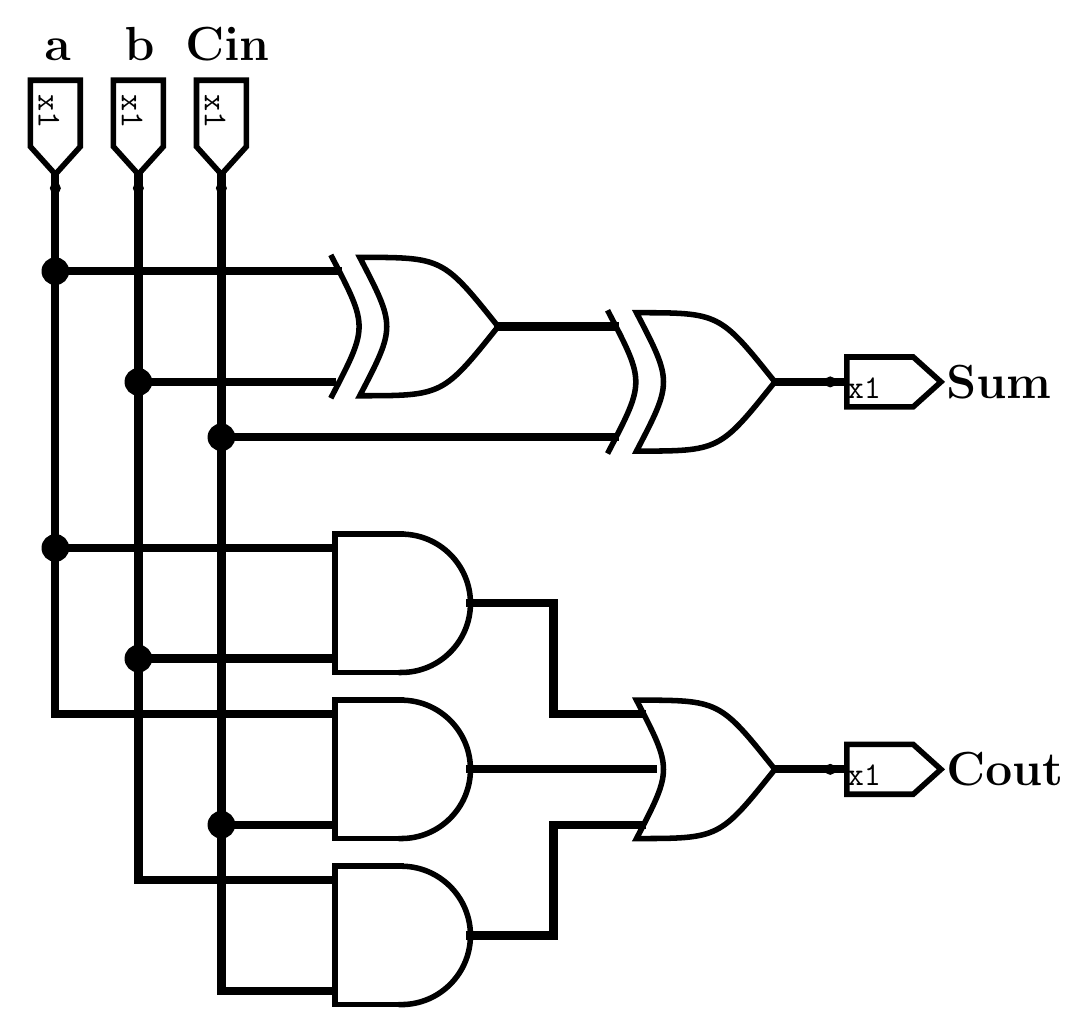
\begin{tikzpicture}[x=1pt,y=-1pt,line cap=rect]
\def\logisimfontA#1{\fontfamily{cmr}{#1}} % Replaced by logisim, original font was "SansSerif"
\def\logisimfontB#1{\fontfamily{cmtt}{#1}} % Replaced by logisim, original font was "Monospaced"
\definecolor{custcol_0_0_0}{RGB}{0, 0, 0}
\definecolor{custcol_ff_ff_ff}{RGB}{255, 255, 255}
\draw [line width=3.0pt, custcol_0_0_0 ]  (15.0,94.0) -- (15.0,194.0) -- (115.0,194.0) ;
\draw [line width=3.0pt, custcol_0_0_0 ]  (275.0,134.0) -- (295.0,134.0) ;
\draw [line width=3.0pt, custcol_0_0_0 ]  (275.0,274.0) -- (295.0,274.0) ;
\draw [line width=3.0pt, custcol_0_0_0 ]  (15.0,194.0) -- (15.0,254.0) -- (115.0,254.0) ;
\draw [line width=3.0pt, custcol_0_0_0 ]  (75.0,294.0) -- (75.0,354.0) -- (115.0,354.0) ;
\draw [line width=3.0pt, custcol_0_0_0 ]  (45.0,234.0) -- (115.0,234.0) ;
\fill [line width=3.0pt, custcol_0_0_0]  (45.0,134.0) ellipse (5.0 and 5.0 );
\fill [line width=3.0pt, custcol_0_0_0]  (15.0,194.0) ellipse (5.0 and 5.0 );
\fill [line width=3.0pt, custcol_0_0_0]  (75.0,154.0) ellipse (5.0 and 5.0 );
\fill [line width=3.0pt, custcol_0_0_0]  (15.0,94.0) ellipse (5.0 and 5.0 );
\fill [line width=3.0pt, custcol_0_0_0]  (75.0,294.0) ellipse (5.0 and 5.0 );
\fill [line width=3.0pt, custcol_0_0_0]  (45.0,234.0) ellipse (5.0 and 5.0 );
\draw [line width=3.0pt, custcol_0_0_0 ]  (75.0,59.0) -- (75.0,64.0) -- (75.0,154.0) -- (75.0,294.0) -- (115.0,294.0) ;
\draw [line width=2.0pt, custcol_0_0_0 ]  (66.0,49.0) -- (75.0,59.0) -- (84.0,49.0) -- (84.0,25.0) -- (66.0,25.0) -- cycle;
\logisimfontB{\fontsize{12pt}{12pt}\selectfont\node[inner sep=0, outer sep=0, custcol_0_0_0, anchor=base west, rotate=-90.0] at  (69.0,30.0)  {x1};}
\logisimfontA{\fontsize{16pt}{16pt}\fontseries{bx}\selectfont\node[inner sep=0, outer sep=0, custcol_0_0_0, anchor=base west] at  (62.0,18.0)  {Cin};}
\fill [line width=2.0pt, custcol_0_0_0]  (75.0,64.0) ellipse (2.0 and 2.0 );
\draw [line width=2.0pt, custcol_0_0_0 ]  (6.0,49.0) -- (15.0,59.0) -- (24.0,49.0) -- (24.0,25.0) -- (6.0,25.0) -- cycle;
\logisimfontB{\fontsize{12pt}{12pt}\selectfont\node[inner sep=0, outer sep=0, custcol_0_0_0, anchor=base west, rotate=-90.0] at  (9.0,30.0)  {x1};}
\logisimfontA{\fontsize{16pt}{16pt}\fontseries{bx}\selectfont\node[inner sep=0, outer sep=0, custcol_0_0_0, anchor=base west] at  (11.0,18.0)  {a};}
\fill [line width=2.0pt, custcol_0_0_0]  (15.0,64.0) ellipse (2.0 and 2.0 );
\draw [line width=2.0pt, custcol_0_0_0] (140.0,359.0) arc (90.0:-90.0:25.0 and 25.0 );
\draw [line width=2.0pt, custcol_0_0_0 ]  (140.0,309.0) -- (116.0,309.0) -- (116.0,359.0) -- (140.0,359.0) ;
\draw [line width=3.0pt, custcol_0_0_0 ]  (165.0,214.0) -- (195.0,214.0) -- (195.0,254.0) -- (225.0,254.0) -- (227.0,254.0) ;
\draw [line width=3.0pt, custcol_0_0_0 ]  (165.0,274.0) -- (225.0,274.0) -- (231.0,274.0) ;
\draw [line width=3.0pt, custcol_0_0_0 ]  (165.0,334.0) -- (195.0,334.0) -- (195.0,294.0) -- (225.0,294.0) -- (227.0,294.0) ;
\draw [line width=2.0pt, custcol_0_0_0 ]  (275.0,274.0) .. controls  (255.0,249.0)  ..  (225.0,249.0) .. controls  (238.0,274.0)  ..  (225.0,299.0) .. controls  (255.0,299.0)  ..  (275.0,274.0) -- cycle ;
\draw [line width=3.0pt, custcol_0_0_0 ]  (175.0,114.0) -- (215.0,114.0) -- (217.0,114.0) ;
\draw [line width=3.0pt, custcol_0_0_0 ]  (75.0,154.0) -- (215.0,154.0) -- (217.0,154.0) ;
\draw [line width=2.0pt, custcol_0_0_0 ]  (275.0,134.0) .. controls  (255.0,109.0)  ..  (225.0,109.0) .. controls  (238.0,134.0)  ..  (225.0,159.0) .. controls  (255.0,159.0)  ..  (275.0,134.0) -- cycle ;
\draw [line width=2.0pt, custcol_0_0_0 ]  (215.0,109.0) .. controls  (228.0,134.0)  ..  (215.0,159.0) ;
\draw [line width=3.0pt, custcol_0_0_0 ]  (299.0,134.0) -- (296.0,134.0) ;
\draw [line width=2.0pt, custcol_0_0_0 ]  (325.0,125.0) -- (335.0,134.0) -- (325.0,143.0) -- (301.0,143.0) -- (301.0,125.0) -- cycle;
\logisimfontB{\fontsize{12pt}{12pt}\selectfont\node[inner sep=0, outer sep=0, custcol_0_0_0, anchor=base west] at  (301.0,140.0)  {x1};}
\logisimfontA{\fontsize{16pt}{16pt}\fontseries{bx}\selectfont\node[inner sep=0, outer sep=0, custcol_0_0_0, anchor=base west] at  (337.0,140.0)  {Sum};}
\fill [line width=2.0pt, custcol_0_0_0]  (295.0,134.0) ellipse (2.0 and 2.0 );
\draw [line width=3.0pt, custcol_0_0_0 ]  (45.0,59.0) -- (45.0,64.0) -- (45.0,134.0) -- (45.0,234.0) -- (45.0,314.0) -- (115.0,314.0) ;
\draw [line width=2.0pt, custcol_0_0_0 ]  (36.0,49.0) -- (45.0,59.0) -- (54.0,49.0) -- (54.0,25.0) -- (36.0,25.0) -- cycle;
\logisimfontB{\fontsize{12pt}{12pt}\selectfont\node[inner sep=0, outer sep=0, custcol_0_0_0, anchor=base west, rotate=-90.0] at  (39.0,30.0)  {x1};}
\logisimfontA{\fontsize{16pt}{16pt}\fontseries{bx}\selectfont\node[inner sep=0, outer sep=0, custcol_0_0_0, anchor=base west] at  (40.0,18.0)  {b};}
\fill [line width=2.0pt, custcol_0_0_0]  (45.0,64.0) ellipse (2.0 and 2.0 );
\draw [line width=2.0pt, custcol_0_0_0] (140.0,299.0) arc (90.0:-90.0:25.0 and 25.0 );
\draw [line width=2.0pt, custcol_0_0_0 ]  (140.0,249.0) -- (116.0,249.0) -- (116.0,299.0) -- (140.0,299.0) ;
\draw [line width=3.0pt, custcol_0_0_0 ]  (299.0,274.0) -- (296.0,274.0) ;
\draw [line width=2.0pt, custcol_0_0_0 ]  (325.0,265.0) -- (335.0,274.0) -- (325.0,283.0) -- (301.0,283.0) -- (301.0,265.0) -- cycle;
\logisimfontB{\fontsize{12pt}{12pt}\selectfont\node[inner sep=0, outer sep=0, custcol_0_0_0, anchor=base west] at  (301.0,280.0)  {x1};}
\logisimfontA{\fontsize{16pt}{16pt}\fontseries{bx}\selectfont\node[inner sep=0, outer sep=0, custcol_0_0_0, anchor=base west] at  (337.0,280.0)  {Cout};}
\fill [line width=2.0pt, custcol_0_0_0]  (295.0,274.0) ellipse (2.0 and 2.0 );
\draw [line width=2.0pt, custcol_0_0_0] (140.0,239.0) arc (90.0:-90.0:25.0 and 25.0 );
\draw [line width=2.0pt, custcol_0_0_0 ]  (140.0,189.0) -- (116.0,189.0) -- (116.0,239.0) -- (140.0,239.0) ;
\draw [line width=3.0pt, custcol_0_0_0 ]  (15.0,59.0) -- (15.0,64.0) -- (15.0,94.0) -- (115.0,94.0) -- (117.0,94.0) ;
\draw [line width=3.0pt, custcol_0_0_0 ]  (45.0,134.0) -- (115.0,134.0) -- (115.0,134.0) ;
\draw [line width=2.0pt, custcol_0_0_0 ]  (175.0,114.0) .. controls  (155.0,89.0)  ..  (125.0,89.0) .. controls  (138.0,114.0)  ..  (125.0,139.0) .. controls  (155.0,139.0)  ..  (175.0,114.0) -- cycle ;
\draw [line width=2.0pt, custcol_0_0_0 ]  (115.0,89.0) .. controls  (128.0,114.0)  ..  (115.0,139.0) ;
\end{tikzpicture}
}

			\label{fig:somadorcompleto2}
		\end{figure}
	\end{columns}
\end{frame}

\begin{frame}
	\frametitle{Somador completo}
	\framesubtitle{\textbf{Demonstração}}
	\par Vamos fazer um somador completo no logisim.
\end{frame}

\begin{frame}
	\frametitle{Mini prova 04}
	\par Altere o circuito somador completo para que o mesmo tenha um modo somador e um modo subtrator.
\end{frame}







%	\begin{frame}[allowframebreaks]
%		\frametitle{Referências}
%		\bibliography{bibliography.bib}
%	\end{frame}
	
\end{document}